%!TEX root = ../TAMUTemplate.tex
%%%%%%%%%%%%%%%%%%%%%%%%%%%%%%%%%%%%%%%%%%%%%%%%%%%
%
%  New template code for TAMU Theses and Dissertations starting Fall 2016.
%
%  Author: Sean Zachary Roberson
%	 Version 3.16.09
%  Last updated 9/12/2016
%
%%%%%%%%%%%%%%%%%%%%%%%%%%%%%%%%%%%%%%%%%%%%%%%%%%%
%%%%%%%%%%%%%%%%%%%%%%%%%%%%%%%%%%%%%%%%%%%%%%%%%%%%%%%%%%%%%%%%%%%%%%
%%                           SECTION V
%%%%%%%%%%%%%%%%%%%%%%%%%%%%%%%%%%%%%%%%%%%%%%%%%%%%%%%%%%%%%%%%%%%%%



\chapter{\texorpdfstring{\uppercase {Higgs Analysis}}{Higgs Analysis}}
\label{ch:analysis}

Data collected by the CMS detector at the LHC is analyzed for the presence of a Higgs boson decaying to the \lvjj final state.
Signal and background Monte Carlo (MC) samples are used to study the efficacy of various object and event selection criteria.
While the signal samples are fully MC based, some of the background samples use data-driven techniques, which will be discussed later in this chapter.
The matrix element probabilities for an event final state being created by a specific diagram are computed.
Several multivariate techniques are studied and used to distinguish between signal-like and background-like events.
We use the discriminator outputs from these multivariate classifiers to set limits on the SM \HWW cross section.

\section{Data and Monte Carlo Samples}

%The following sections will describe the datasets collected by CMS as well as the MC samples used in this analysis.

\subsection{Data}
\label{sec:data}

As mentioned previously, this analysis makes use of the full 2012 CMS dataset of 8\tev data.
Fig.~\ref{fig:int_lumi_per_day} shows the cumulative delivered, recorded, and validated luminosity versus time.
Only fully validated data, where both the LHC and CMS are completely operational, are use used for CMS analyses~\cite{LumiPublic}.
Table~\ref{tab:dataSamples} shows the data samples used for this analysis, which corresponds to $\sim$19.2\fbinv.
The datasets are split by the two HLT paths used, one which selects for a single high \pt electron and one for a single high \pt muon.
These two separate PDs correspond to the HLT\_Ele27\_WP80\_v* and HLT\_IsoMu24\_eta2p1\_v* trigger paths, respectively.
The HLT\_Ele27\_WP80\_v* path requires a reconstructed electron with \ptgt{27}\gev along with several other criteria grouped into a working point with 80\% efficiency of selecting true electrons.
The HLT\_IsoMu24\_eta2p1\_v* criteria requires an isolated, reconstructed muon with \ptgt{24}\gev within \absetalt{2.1}.
The luminosities listed in the table are associated with a 2.6\% uncertainty as specified in~\cite{CMS-PAS-LUM-12-001} and were collected using the HF luminosity measurements~\cite{CMS-PAS-LUM-13-001}.

\begin{figure}[!hbt]
    \centering
    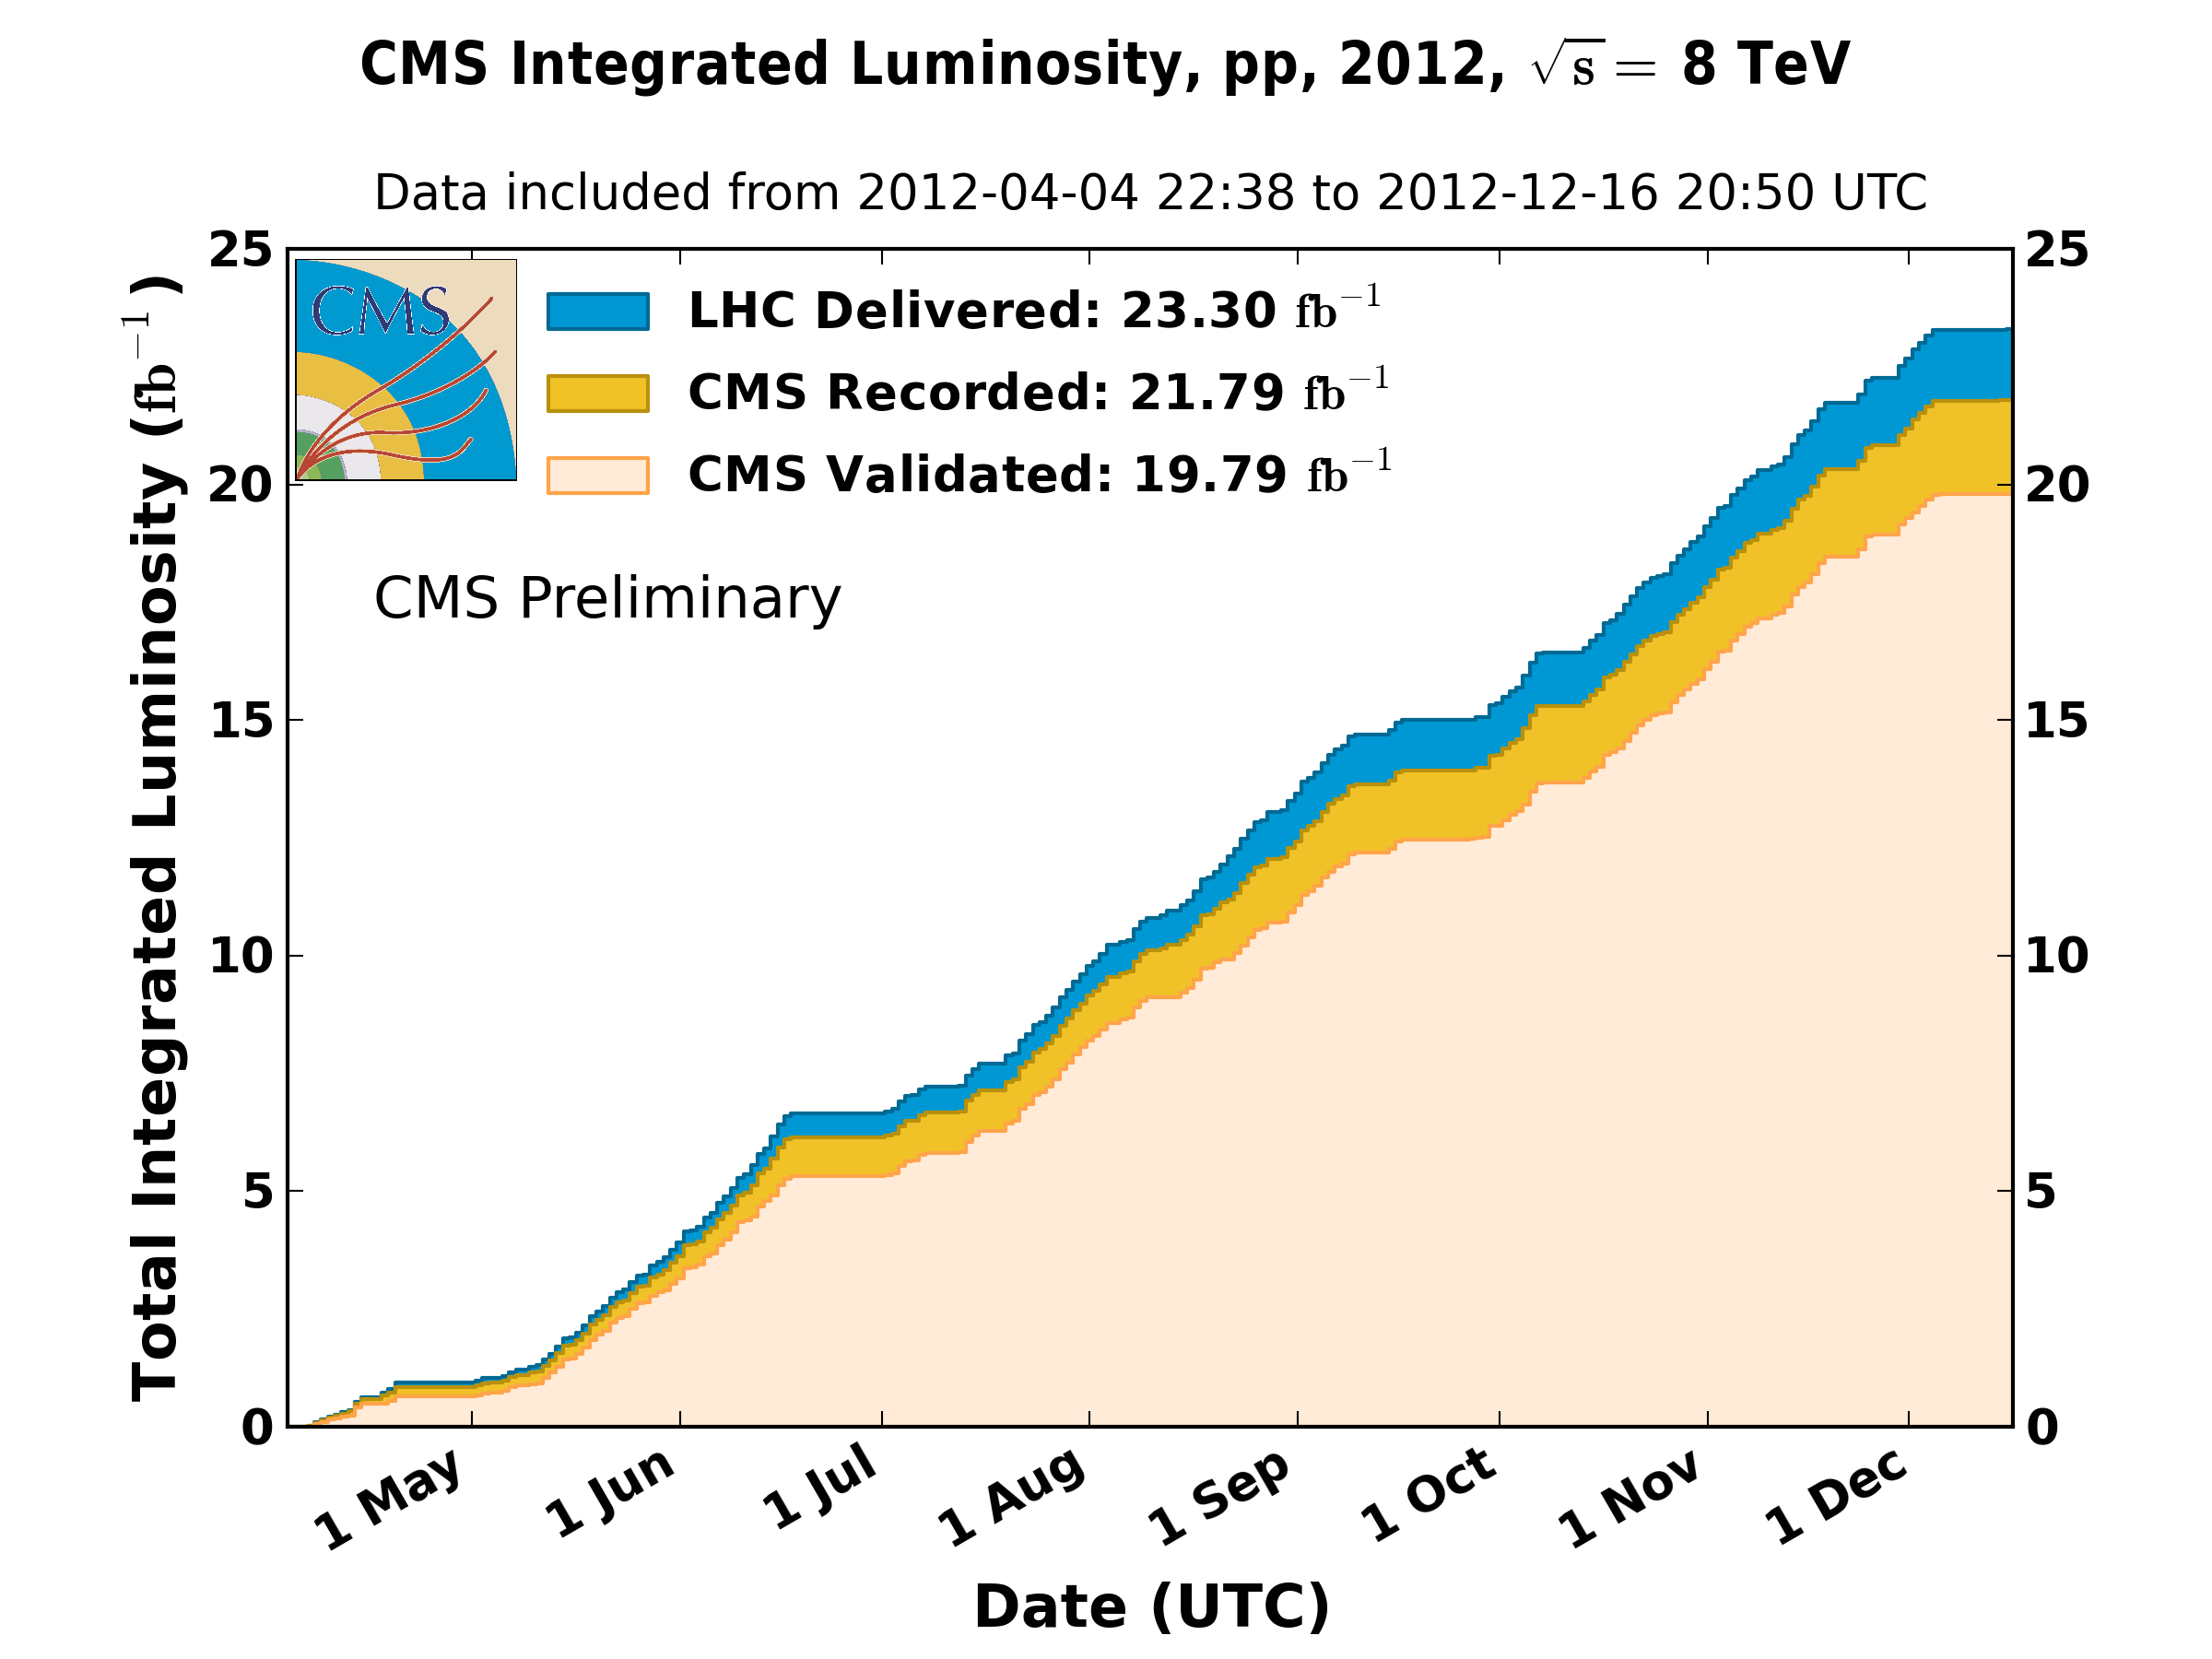
\includegraphics[width=0.95\textwidth]{\figpath/Chapter5/int_lumi_per_day_cumulative_pp_2012_SummerConf.png}
    \caption{Cumulative day-by-day integrated luminosity in 2012 delivered by the LHC (blue), recorded by CMS (dark orange), and validated for physics use (light orange)~\cite{DataQuality}.}
    \label{fig:int_lumi_per_day}
\end{figure}

\begin{table}[hbtp]\footnotesize
\centering
\begin{tabular}{l l l}
\hline
 Dataset & Run Range & Integrated Luminosity \\
\hline
/SingleMu/Run2012A-13Jul2012-v1/AOD & 190645-196531 & 0.809$\fbinv$ \\
/SingleMu/Run2012A-recover-06Aug2012-v1/AOD & 190782-190949 & 0.082$\fbinv$ \\
/SingleMu/Run2012B-13Jul2012-v1/AOD & 193834-196531 & 4.383$\fbinv$ \\
/SingleMu/Run2012C-24Aug2012-v1/AOD & 198022-198523 & 0.489$\fbinv$ \\
/SingleMu/Run2012C-PromptReco-v2/AOD & 194631-203002 & 6.285$\fbinv$ \\
/SingleMu/Run2012D-PromptReco-v1/AOD & 194480-208686 & 7.231$\fbinv$ \\
{\bf Total SingleMu} & {\bf 190645--208686} & {\bf 19.279$\fbinv$} \\
\hline
/SingleElectron/Run2012A-13Jul2012-v1/AOD & 190645-196531 & 0.809$\fbinv$ \\
/SingleElectron/Run2012A-recover-06Aug2012-v1/AOD & 190782-190949 & 0.082$\fbinv$ \\
/SingleElectron/Run2012B-13Jul2012-v1/AOD & 193834-196531 & 4.336$\fbinv$ \\
/SingleElectron/Run2012C-24Aug2012-v1/AOD & 198022-198523 & 0.489$\fbinv$ \\
/SingleElectron/Run2012C-PromptReco-v2/AOD & 194631-203002 & 6.194$\fbinv$ \\
/SingleElectron/Run2012D-PromptReco-v1/AOD & 194480-208686 & 7.238$\fbinv$\\
{\bf Total SingleElectron} & {\bf 190645--208686} & {\bf 19.148$\fbinv$} \\
\hline
\end{tabular}
\caption{The datasets analyzed for this analysis.}
\label{tab:dataSamples}
\end{table}

\subsection{Monte Carlo}

This analysis makes use of MC simulation to study the background processes which have similar final states to that of the \HWWlvjj signal.
Both the kinematic distributions and the final yields are extracted from these samples.
The MC simulation is used for all backgrounds except for the multijet process, where a data-driven approach is used instead.
The process of developing this sample is described in detail in the section~\ref{sec:QCD_data-driven_sample}.
The signal sample kinematics and yields are also taken from MC.
Tables~\ref{tab:SignalSamples} and~\ref{tab:bkgSamples} list all of the MC sample for the Higgs signals and SM background processes, respectively.
The SM background and volunteer signal samples are centrally produced by the CMS collaboration.
The \ggH samples were produced specifically for this analysis.
All of the samples, regardless of who produced them, are stored in a database called the Data Aggregation System (DAS) and organized by the ``Dataset Name'' field.
The backgrounds were modeled by MC samples generated with \textsc{MadGraph}~\cite{Alwall:2014hca} and \textsc{pythia6}~\cite{1126-6708-2006-05-026}. 
The signal MC samples were also generated by \textsc{pythia6}.
Tables~\ref{tab:bkgSamples} and~\ref{tab:SignalSamples} list all of the MC for the Higgs signal and SM background processes, respectively.

\begin{sidewaystable}[hbtp]\footnotesize
\centering
\begin{tabular}{l p{0.50\textwidth} l l}
\hline
\multicolumn{4}{c}{Signal Processes} \\
\hline
Production \& Decay Modes & Dataset Name & Cross Section [\unit{pb}] & BR\\  \hline
\ggH; $\MH=\text{125}\gev$, \HWWlvjj & /LQ-ggh125\_BIG\_SIM\_ggH125\_part1/aperloff-LQ-ggh125\_AODSIM\_Summer12\_START53\_V7E-{\newline}768a14b04b0ac2af0d20e6783fbdb759/USER & 19.27 & 0.0947 \\
  & /LQ-ggh125\_BIG\_GEN\_part2/aperloff-LQ-ggh125\_BIG\_RECO\_part2-33e909ff21293ad9fa8564de2959fe54/USER & 19.27 & 0.0947\\
  & /LQ-ggh125\_BIG\_GEN\_part3/aperloff-LQ-ggh125\_BIG\_RECO\_part3-33e909ff21293ad9fa8564de2959fe54/USER & 19.27 & 0.0947\\
  & /LQ-ggh125\_Part6\_SIM/goodell-LQ-qqh125\_RECO\_Part6-33e909ff21293ad9fa8564de2959fe54/USER & 19.27 & 0.0947\\
  & /LQ-ggh125\_Part7\_SIM/goodell-LQ-qqh125\_RECO\_Part7-33e909ff21293ad9fa8564de2959fe54/USER & 19.27 & 0.0947\\
  & /LQ-ggh125\_Part8\_GENSIM/goodell-LQ-ggh125\_Part8\_RECO-33e909ff21293ad9fa8564de2959fe54/USER & 19.27 & 0.0947\\
\qqH; $\MH=\text{125}\gev$, \HWWlvjj & /LQ-vbf125\_GENSIM/ajkumar-LQ-qqh125\_AODSIM\_Summer12\_{\newline}START53\_V7A-c8f8ed334db8a7d6f56c62266b1dfa5b/USER & 1.578 & 0.0947\\
\WH, \ZH, \ttH; $\MH=\text{125}\gev$, \HWW, inclusive & /WH\_ZH\_TTH\_HToWW\_M-125\_8TeV-pythia6 & 1.249 & 0.215\\\hline
\multicolumn{4}{c}{Non signal Higgs Production} \\ \hline
\WH, \ZH, \ttH; $\MH=\text{125}\gev$, \HZZ, inclusive & /WH\_ZH\_TTH\_HToZZ\_M-125\_8TeV-pythia6 & 1.249 & 0.0264\\
\WH; $\MH=\text{125}\gev$, \Hbb, \Wlv & /WH\_WToLNu\_HToBB\_M-125\_8TeV-powheg-herwigpp & 0.7046 & 0.1879\\
\ttH; $\MH=\text{125}\gev$, \Hbb & /TTH\_HToBB\_M-125\_8TeV-pythia6 & 0.1293 & 0.577\\
\hline
\end{tabular}
\caption{List of signal datasets and cross sections. All of the centrally produced sample names are followed by /Summer12\_DR53X-PU\_S10\_START53\_V7A-v1/AODSIM.}
\label{tab:SignalSamples}
\end{sidewaystable}

\begin{sidewaystable}[hbtp]\footnotesize
\centering
\begin{tabular}{l p{0.65\textwidth} l}
\hline
\multicolumn{3}{c}{Background Processes} \\
\hline
Process & Dataset Name & Cross Section [\unit{pb}] \\
\hline
\Wjets & /WJetsToLNu\_TuneZ2Star\_8TeV-madgraph-tarball & 37509 \\
\ttbar & /TTJets\_MassiveBinDECAY\_TuneZ2star\_8TeV-madgraph-tauola & 225.197 \\
\Zjets & /DYJetsToLL\_M-50\_TuneZ2Star\_8TeV-madgraph-tarball & 3387.6 \\
\WW & /WW\_TuneZ2star\_8TeV\_pythia6\_tauola & 54.838 \\
\WZ & /WZ\_TuneZ2star\_8TeV\_pythia6\_tauola & 33.21 \\
\ZZ & /ZZ\_TuneZ2star\_8TeV\_pythia6\_tauola & 17.654 \\
$\cPqt\rightarrow\cPqb\ell\nu$ (\cPqs-channel) & /T\_s-channel\_TuneZ2star\_8TeV-powheg-tauola & 3.79 \\
$\cPqt\rightarrow\cPqb\ell\nu$ (\cPqt-channel) & /T\_t-channel\_TuneZ2star\_8TeV-powheg-tauola & 56.4 \\
$\cPqt\rightarrow{X}$ (\cPqt\W-channel) & /T\_tW-channel-DR\_TuneZ2star\_8TeV-powheg-tauola & 11.1 \\
$\cPaqt\rightarrow\cPqb\ell\nu$ (\cPqs-channel) & /Tbar\_s-channel\_TuneZ2star\_8TeV-powheg-tauola & 1.76 \\
$\cPaqt\rightarrow\cPqb\ell\nu$ (\cPqt-channel) & /Tbar\_t-channel\_TuneZ2star\_8TeV-powheg-tauola & 30.7 \\
$\cPaqt\rightarrow{X}$ (\cPqt\W-channel) & /Tbar\_tW-channel-DR\_TuneZ2star\_8TeV-powheg-tauola & 11.1 \\
QCD (\Pe-channel) & See table~\ref{tab:dataSamples} for a list of SingleElectron datasets & N/A \\
QCD (\Pmu-channel) & See table~\ref{tab:dataSamples} for a list of SingleMu datasets & N/A \\
\hline
\end{tabular}
\caption{List of background MC datasets and cross sections used in the analysis. Every dataset name is followed by /Summer12\_DR53X-PU\_S10\_START53\_V7A-v1/AODSIM. In addition to v1, this analysis also uses v2 of the \Wjets sample.}
\label{tab:bkgSamples}
\end{sidewaystable}

The \ttbar, \Wjets, and \Zjets SM background samples are generated using \textsc{Mad}\textsc{Graph} v5.1.3.30~\cite{Alwall:2014hca}.
The \ttbar sample is inclusive, meaning that it includes all decay modes of the \W boson coming from the top decay.
The \Wjets and \Zjets samples are also inclusive, but in this case it means that in addition to the leptonic decay of the boson there are any number of final state jets.
The single top quark samples are modeled using the \textsc{POWHEG} 1.0 r138 ~\cite{POWHEG2,POWHEG:singlet,POWHEG:singletW} generator.
The diboson processes use the \textsc{pythia} v6.4.24 generator~\cite{1126-6708-2006-05-026}.
The cross sections for the \ttbar and single top quark processes are calculated at next-to-next-to-leading logarithmic (NNLL) accuracy~\cite{TOPCrossSec} while the inclusive \Wjets and \Zjets processes are calculated at next-to-next-to-leading order (NNLO) accuracy~\cite{FEWZ}.
The diboson cross sections are calculated at next-to-leading order (NLO) accuracy~\cite{MCFM}.

The \HWW signal samples are generated with \textsc{pythia} v6.4.24~\cite{1126-6708-2006-05-026}, where one \W is required to decay leptonically while the other is required to decay hadronically.
The cross sections for the Higgs production are calculated at NNLL QCD and NLO EW accuracies.
The calculations for gluon-gluon fusion and VBF production cross sections use the complex-pole-scheme (CPS) while the associated production cross section are calculated with the zero-width-approximation (ZWA)~\cite{Heinemeyer:2013tqa}.
These samples were privately produced because the centrally produces samples did not include enough events and had large statistical fluctuations.

\subsection{Multijet-QCD Background}
\label{sec:QCD_data-driven_sample}

It is well known that the QCD process is difficult to model to the desired level of accuracy.
Additionally, the event selection in this analysis requires two isolated jets and an isolated lepton, which vastly reduces the number of QCD MC events that pass the selection criteria.
Although the probability to mis-reconstruct a jet as a lepton is fairly low, the production cross section for the multijet process is extremely high and thus cannot be ignored.
When using the MC samples we are left with a statistically limited sample that is almost useless for describing this background.

Rather than relying on MC for the QCD background sample, a data-driven sample was created by using the same trigger requirements as the data, but removing the isolation requirement for the lepton and inverting the lepton particle flow isolation cut during selection.
The main idea of the method is to utilize differences in lepton identification properties that separate prompt, isolated leptons from \W and \Z decays, also known as ``real leptons,'' from non-prompt, non-isolated leptons, also known as ``fake leptons.''
The normal signal selection requires an isolated lepton, without other particles around it, to limit this sort of ``fake lepton,'' but this is exactly the type of property we want to select for when forming a QCD sample from data.
This process provides a completely orthogonal sample of QCD events from data that won't, and shouldn't be used for signal extraction.
Since we make use of the entire 2012 dataset\footnote{The QCD events are scaled slightly to account for failed jobs (missing luminosity) during processing.}, we end up with statistically rich samples containing lots of mis-identified leptons.

A complete description of the event selection will be discussed in section~\ref{ch:event_selection}, but here I will just talk about the isolation requirements.
The loosest lepton PF isolation requirement used to determine the signal region is $\pfiso<0.2$, which is used to veto on ``loose'' or questionable leptons.
The assumption is that any lepton with $\pfiso>0.2$ is a mis-reconstructed lepton coming from QCD.
For electrons we must also turn off the MVA-based identification requirements as they are stringent enough that they won't allow for any fake leptons to pass our selection.
As mentioned before, the electrons must still pass the ``HLT\_Ele27\_WP80\_v*'' electron trigger used for the data containing our signal.
On the other hand, the muon trigger is changed to be ``HLT\_Mu24\_eta2p1\_v*'' to remove the isolation requirement that was included in the trigger used to select for the signal.

In order to gain greater separation from the signal selection to ensure as little non-QCD contamination as possible, we actually use a minimum isolation requirement of $\pfiso>0.3$.
We also put an upper limit on the PF isolation value to keep the sample from having a bias towards high nPV values.
For electrons the upper limit was 0.7 and for muons it was 2.0.
The $1\sigma$ systematic uncertainty bands for electrons (muons) were selected to be $0.2<\pfiso<0.3$ on the low side and $>$0.7 (2.0) for the high side
Fig.~\ref{fig:PFIsolation} shows the pf isolation values contained in the electron multijet and data samples as a function of $\eta$.

\begin{figure}[!hbt]
    \centering
    \begin{subfigure}[t]{0.475\textwidth}
        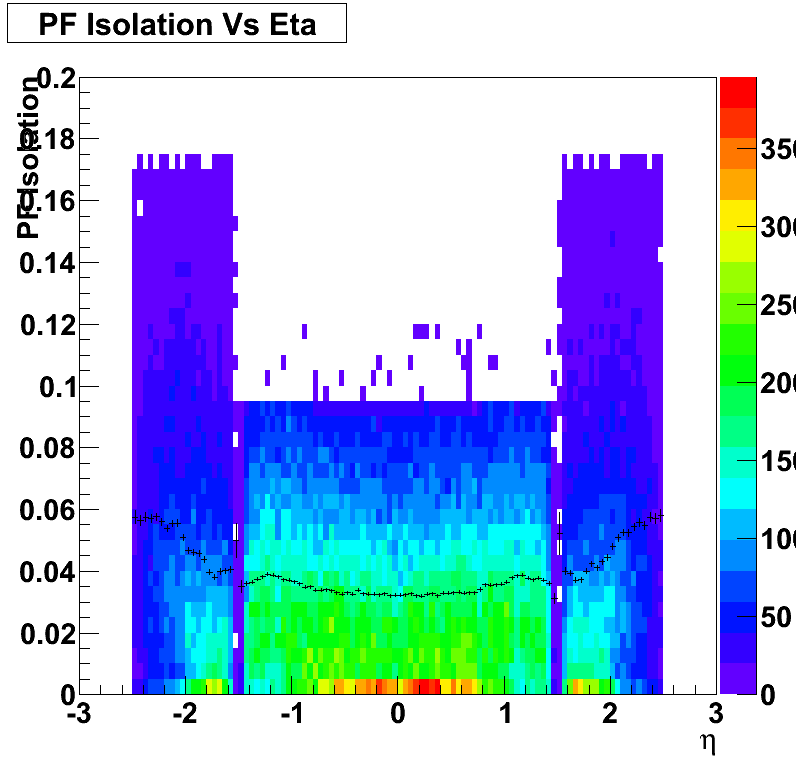
\includegraphics[width=\textwidth]{\figpath/Chapter5/pfIsoVsEta_DATA.png}
        \caption{}
        \label{fig:PFIsolationData}
    \end{subfigure}
    \begin{subfigure}[t]{0.475\textwidth}
        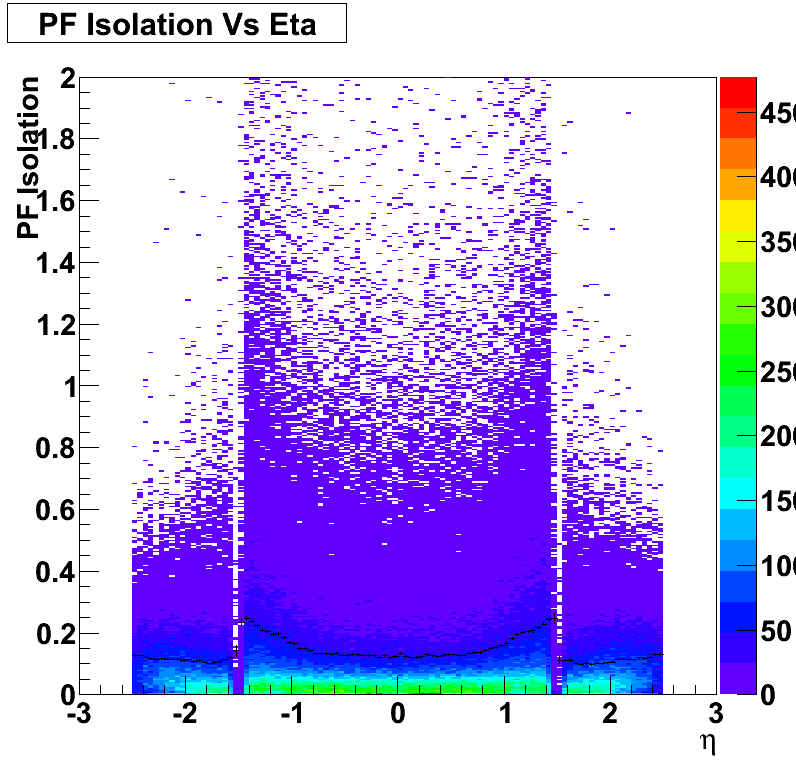
\includegraphics[width=\textwidth]{\figpath/Chapter5/pfIsoVsEta_Full.png}
        \caption{}
        \label{fig:PFIsolationFull}
    \end{subfigure}
    \caption{The PF isolation for the electron channel as a function of $\eta$ (left) with and (right) without the lepton isolation and electron MVA-based identification requirements.}
    \label{fig:PFIsolation}
\end{figure}

\section{Event \& Object Selection}
\label{ch:event_selection}

The reconstruction algorithms described in chapter~\ref{ch:event_reconstruction} are designed to be fairly generic and applicable to a wide array of physics analyses.
Specific groups within CMS called physics object groups (POGs) are responsible for developing object quality criteria which must be implemented by each analysis to prevent fake or poorly reconstructed objects.
This section will discuss the object selection criteria used to identify vertices, electrons, muons, jets, and \VETslash, which all meet or exceed the object requirements as set by the relevant POGs.
Only events which have the right quality and multiplicities of these objects will be used in the analysis.

Like most analyses, this one selects for a single good quality primary vertex, although the presence of additional vertices (pileup) does not disqualify the event.
The primary vertex must pass certain additional quality criteria.
There must be at least four degrees of freedom used to find the vertex, the absolute value of the $z$-coordinate of the vertex must be less than 24\unit{cm}, the absolute value of the $\rho$-coordinate (cylindrical coordinate system) must be less than 2.0\unit{cm}, and the vertex must not be identified as a fake vertex.
These criteria are summarized in table~\ref{tab:vertex_selection}.

\begin{table}[hbtp]\footnotesize
\centering
\begin{tabular}{l l}
\hline
Cut & Value \\
\hline
N\textsubscript{DOF} & $\geqslant$4 \\
$|z|$ & $\leqslant$24\unit{cm} \\
$|\rho|$ & $\leqslant$2.0\unit{cm} \\
\hline
\end{tabular}
\caption{The primary vertex selection requirements for this analysis.}
\label{tab:vertex_selection}
\end{table}

As mentioned before, this analysis selects for the presence of one lepton, either an electron or muon, at least two jets, and some amount of \VETslash.
In practical terms this means that we select for one tight electron (muon) as defined in section~\ref{sec:electrons} (\ref{sec:muons}) and veto the event if there are any additional tight or loose electrons and muons (muons and electrons).
Some additional cuts beyond those of the identification requirements are imposed to cut out some of the background events while maximizing the number of signal events we could use for the multivariate analysis techniques.
The additional \pt and $\eta$ requirements as specified in the same sections are also applied.
For the tight electrons this meant raising the \pt requirement from 27\gev to 30\gev, which avoids using events right on the trigger turn on threshold while only removing $\sim$5\% of signal events, as seen in fig.~\ref{fig:electronPt_signal_loss}. 
Because muon reconstruction and identification in CMS is very good, we only raised the \pt requirement to 25\gev from 24\gev.

\begin{figure}[!hbt]
    \centering
    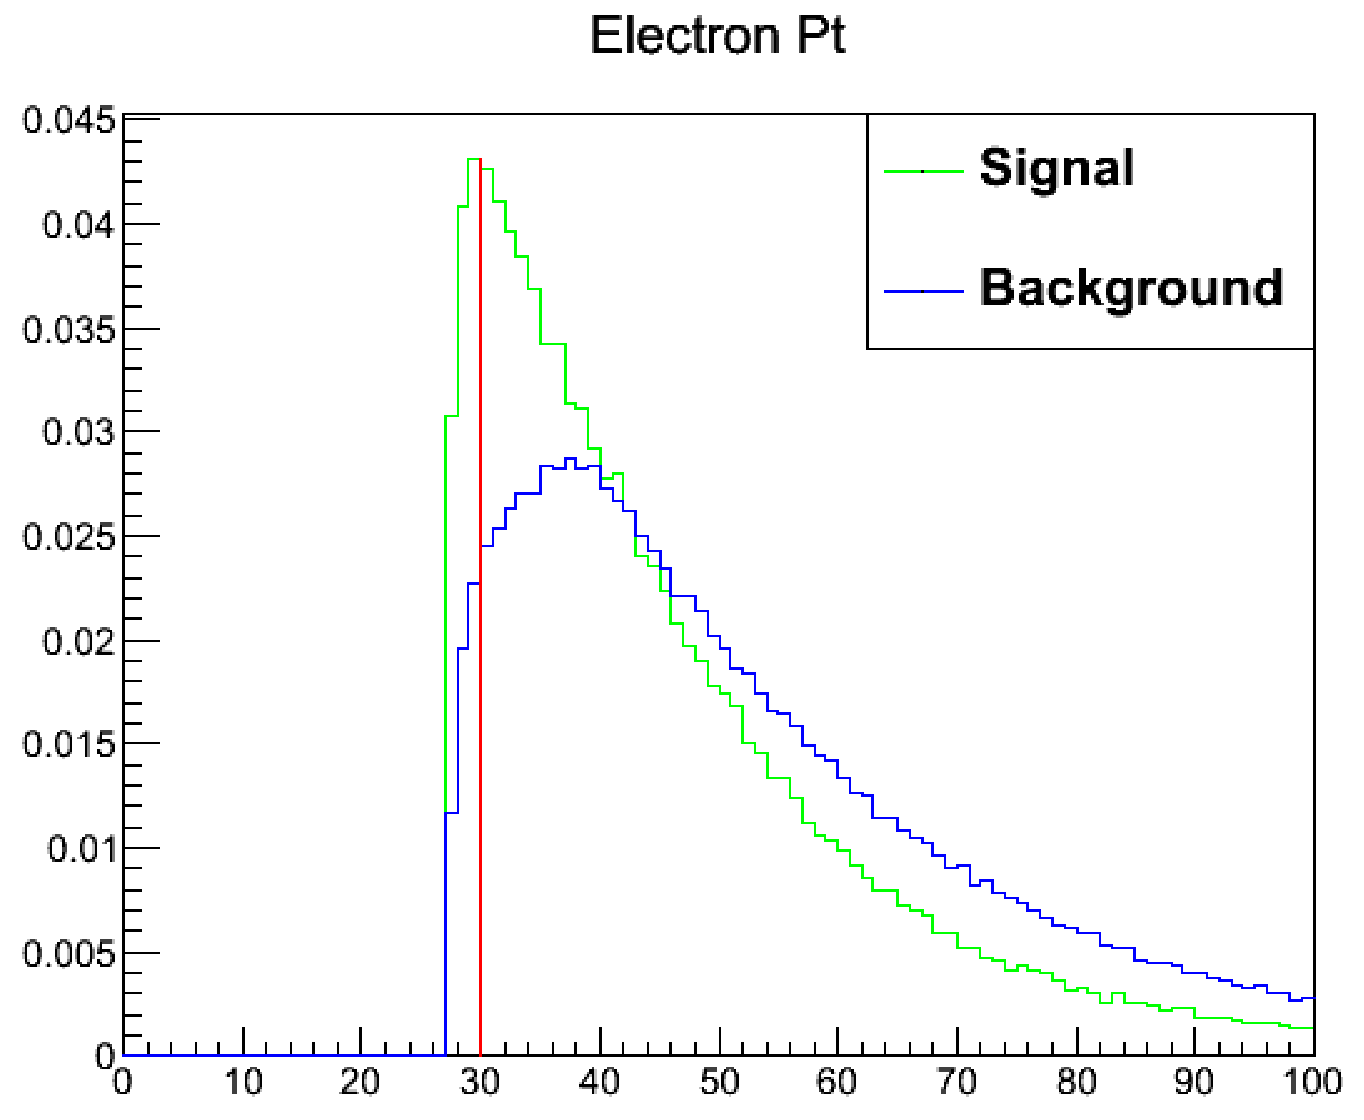
\includegraphics[width=0.95\textwidth]{\figpath/Chapter5/electronPt.png}
    \caption{Histograms of the electron \pt distribution where the gluon-gluon fusion signal is in green and the \Wjets background is in blue. The histograms are normalized to unit area. The red line show the cut on electron \pt where 5\% of the signal is lost.}
    \label{fig:electronPt_signal_loss}
\end{figure}

Beyond the lepton requirements, this analysis selected for any number of jets as long as they pass the selection criteria found in section~\ref{sec:jets}.
As the hadronic W decay will have at least two jets, that is the minimum number of jets needed to make it into the signal region, but we do not veto on additional jets which might come from ISR or FSR.
The requirement of the leading jet having a \ptgt{30}\gev was implemented to reduce the impact of the multijet background while minimally impacting the signal.
Besides the logical splitting of events based on lepton flavor, we also split events into three categories based on the number of jets in the event; exactly two jets, exactly three jets, and four or more jets.
As stated in section~\ref{sec:MET} we also require at least 25\gev of \VETslash.

Given that our signal has only one hadronic \W boson, we don't expect the $\W\rightarrow\bbbar$ branching fraction to contribute much to our signal.
However, we also want to remove as many \ttbar or single top events as possible, which are commonly associated with \cPqb quarks.
Thus we decided to veto events with b-tagged jets in order to reduce our backgrounds as much as possible.
An additional reason to do this is to keep the orthogonality between this analysis and another CMS analysis which was looking at the \VH production channel where \Hbb.
That analysis uses the same final state as this one, but requires two b-tagged jets~\cite{PhysRevD.89.012003}.
To prevent overlap, we only ever considered events with one or fewer b-tagged jets and then we separate the events into two categories based on the number of b-tags.
The zero b-tag events are used for signal extraction while the one b-tag events, which have a much larger impact from \ttbar and a higher \Hbb signal yield, are used for validation purposes and to check the volunteer signal contribution.

%Should I show the cut flow tables for 1-btagged category?

\section{MC Corrections}

Although a significant amount of work and time goes into making sure the MC simulation properly models the data, there can still exist discrepancies between the observed data and simulation
%there are still some corrections which must be made to the reconstructed objects or scale factors which must apply to weight each event in order to accurately mimic the behavior in data.
Often this occurs because the exact data taking conditions are not known in advance, like the pileup conditions that will exist.
Another reason the MC might not exactly mimic the data is that even state of the are generators are limited in their precision; much of the physics of hadronization is still unknown and hard physics processes can often only be computed up to NLO precision.
Data, on the other hand, contains all hadronization effects and all orders of precision.
I have already discussed some object specific corrections like the jet energy corrections, jet energy resolution, and \VETslash corrections in sections~\ref{sec:jets} and~\ref{sec:MET}.
For other discrepancies it is often necessary to reweight the full event rather than a specific object.

Broadly speaking these corrections can be separated into two categories: those which are common to all CMS analyses and those which are specific to this analysis.
The first category includes the b-tagging CSV discriminant weights and top quark \pt spectrum weights for the \ttbar simulation while the second category includes the weights for our multijet sample.
These event weights are applied after selecting for the events as they do not change the object kinematics.

\subsection{Pileup Reweighting}
\label{sec:pileup_reweighting}

Pileup is an important quantity as it can affect the reconstruction efficiency and even the observed kinematics of all the objects used in this analysis.
Up to this point it has been described as additional proton-proton interactions within an event, besides the interaction that produced the physics objects we are interested in studying.
There are several other properties of pileup which are worth noting.
I have so far either referred to pileup in a general sense or as relating to additional objects (tracks or energy) which might be found in the same bunch crossing as the event under study.
In reality there are two different categories of pileup.
There is indeed the pileup which comes from additional proton-proton interactions within the same bunch crossing, known as ``in-time'' pileup.
There is also energy from pileup added to objects because it was left in the sub-detectors from bunch crossings before or after the current one.
This is known as ``out-of-time'' pileup and comes about because the integration window of the sub-detectors can be larger than 25\unit{ns}.
An additional property is somewhat obvious in that the true number of proton-proton interaction within an event, $\mu$, is related to the instantaneous luminosity, which can vary over the course of data taking and even within a luminosity section (LS) period.
As a benchmark, the average number of proton-proton interactions per bunch crossing in 2012 was 21~\cite{LumiPublic}.

\begin{figure}[!hbt]
    \centering
    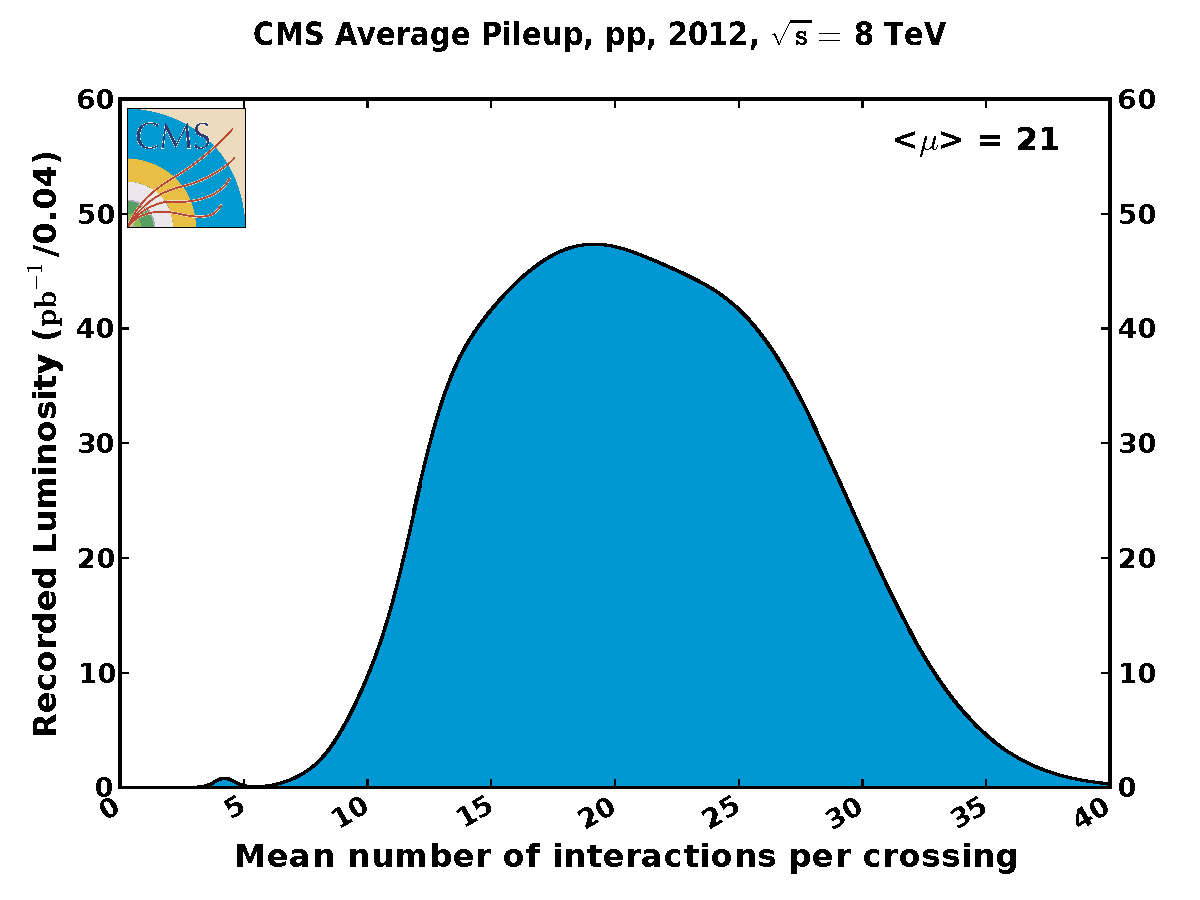
\includegraphics[width=0.95\textwidth]{\figpath/Chapter5/pileup_pp_2012.pdf}
    \caption{The mean number of interactions per bunch crossing in 2012. The min-bias cross section used for the calculation is 80\unit{mb}.}
    \label{fig:pileup_pp_2012}
\end{figure}

The MC samples used in CMS are usually generated before the data is taken and are thus created with an assumption of what the pileup conditions will look like in data.
A broad distribution of $\mu$ values, the number of min-bias pileup events overlaid on the hard scatter event, is generally chosen so as to cover all pileup conditions which might be experienced over the course of a data taking period.
Somewhat unsurprisingly the anticipated $\mu$ distribution rarely matches the one one observed in the data and thus the MC must be reweighted such that the $\mu$ distributions match~\cite{PileupStudiesTwiki}.
To generate a histogram for the average number of interactions per bunch crossing coming from data we make use of the approved pileupCalc tool provided by CMS.
This tool takes as input the total inelastic cross section $\sigma_{\text{inelastic}}=69.3\unit{mb}$\footnote{This is the CMS approved best fit value, not the theoretical value.}, a file in JSON format with every run number and luminosity section matched to a given average instantaneous luminosity and integrated luminosity for that given LS, and another JSON formatted file with the run numbers and LS used in the given analysis\footnote{This analysis uses the full 2012 ``golden'' JSON file called\\Cert\_190456-208686\_8TeV\_PromptReco\_Collisions12\_JSON.txt.}.
All of the MC samples used contain the same $\mu$ distribution scenario denoted by the ``S10'' notation in the dataset name.
The per event weights as a function of $\mu$ are created by dividing the normalized distribution from data by the normalized MC based distribution.
The weights are then applied to each MC event by looking up the weight for the mean number of pileup interactions used to generate that specific event~\cite{PileupWeightTwiki}. The distributions of pileup interactions in MC and data a well as the corresponding pileup weights can be seen in fig.~\ref{fig:pileup_reweighting}. Unfortunately, because the weights are not at unity, the statistical precision of the MC samples is reduced.
Fig.~\ref{fig:npv_comparison} shows the data to MC comparison of the N\textsubscript{PV} distribution before and after the pileup reweighting scheme has been applied.

\begin{figure}[!hbt]
    \centering
    \begin{subfigure}[t]{0.48\textwidth}
      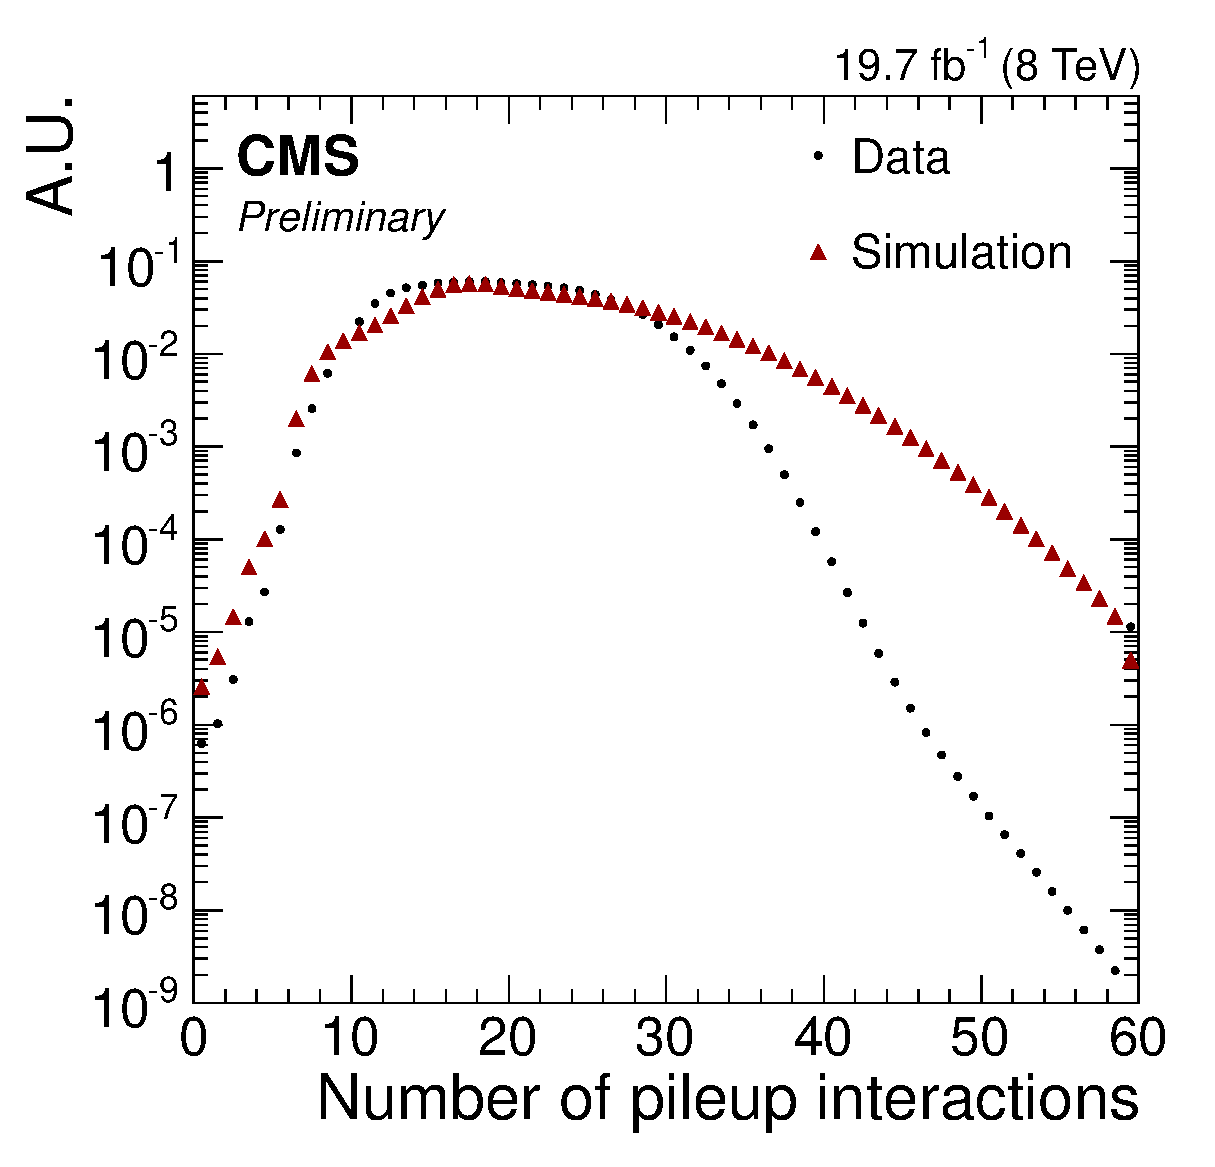
\includegraphics[width=0.95\textwidth]{\figpath/Chapter5/PileupDistribution.eps}
      \caption{}
      \label{fig:tnpu_distributions}
    \end{subfigure}
    \begin{subfigure}[t]{0.48\textwidth}
      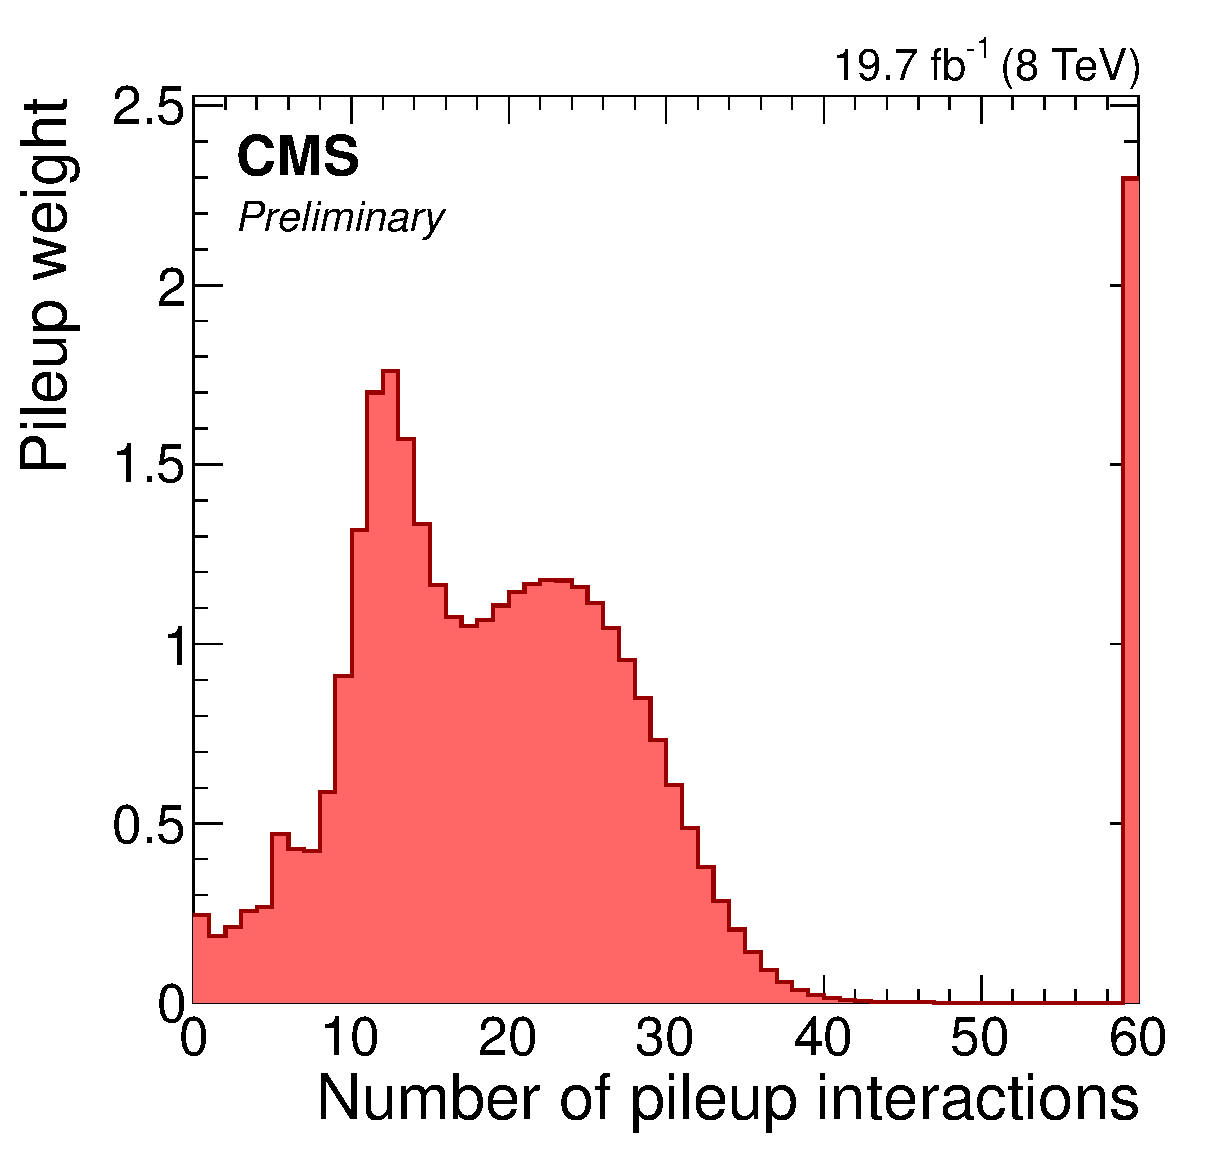
\includegraphics[width=0.95\textwidth]{\figpath/Chapter5/PileupWeights.eps}
      \caption{}
      \label{fig:pileup_weights}
    \end{subfigure}
    \caption{(a) Distributions of the number of pileup interactions in data and in simulation. (b) The derived pileup weights as a function of the number of interactions.}
    \label{fig:pileup_reweighting}
\end{figure}

\begin{figure}[!hbt]
    \centering
    \begin{subfigure}[t]{0.48\textwidth}
      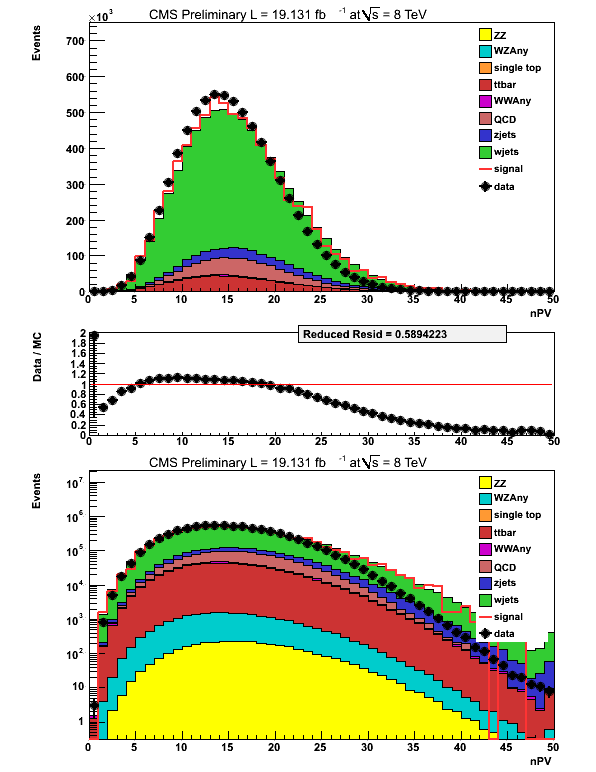
\includegraphics[width=\textwidth]{\figpath/Chapter5/nPV_noRW__comblep.png}
      \caption{}
      \label{fig:npv_no_pileup_reweight}
    \end{subfigure}
    \begin{subfigure}[t]{0.48\textwidth}
      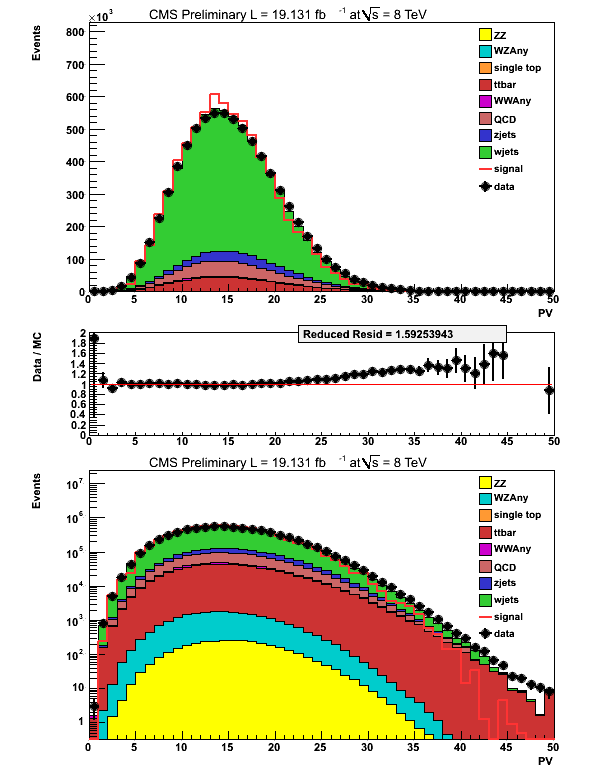
\includegraphics[width=\textwidth]{\figpath/Chapter5/nPV__comblep.png}
      \caption{}
      \label{fig:npv_pileup_reweight}
    \end{subfigure}
    \caption{Comparison of the number of primary vertices (N\textsubscript{PV}) in data and in MC (a) before the the pileup weights are applied and (b) after the weights are applied. These distributions correspond to the 19\fbinv collected during the 2012 data taking period and include both the electron and muon categories.}
    \label{fig:npv_comparison}
\end{figure}

While this methodology is sufficient for the simulated backgrounds, it does not work for the data-driven multijet background.
As can be seen from figs.~\ref{fig:QCDvData_nPV_ele} and~\ref{fig:QCDvData_nPV_mu}, the distributions for the number of primary vertices between data and the QCD samples do not match, indicating some bias due to the selection.
Since the QCD sample does not contain the truth level number of pileup interactions, this is data after all, it would be improper to look up pileup weights using the same weight distribution as for simulation.
Instead, a new set of weights is derived using the number of primary vertices for data in the signal region and anti-isolated region, assuming that the vertex finding efficiency is the same in both regions and only the selection of the lepton changes.
These weights can be seen in figs.~\ref{fig:QCD_PUWeights_ele} and~\ref{fig:QCD_PUWeights_mu} and are applied in the same manner as before.

\begin{figure}[!hbt]
    \centering
    \begin{subfigure}[t]{0.48\textwidth}
        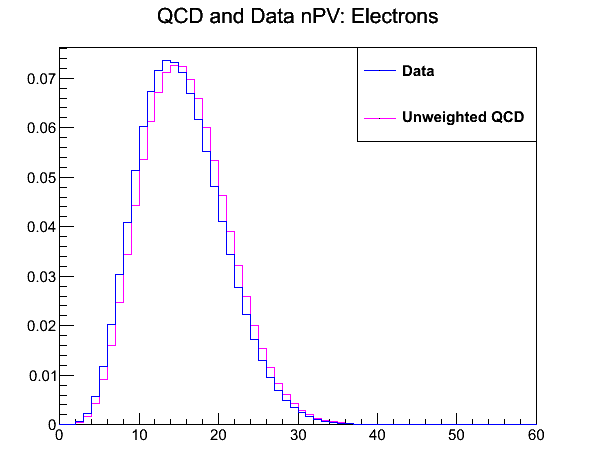
\includegraphics[width=\textwidth]{\figpath/Chapter5/QCD_PUWeights/QCDvData_nPV_ele.png}
        \caption{}
        \label{fig:QCDvData_nPV_ele}
    \end{subfigure}
    \begin{subfigure}[t]{0.48\textwidth}
        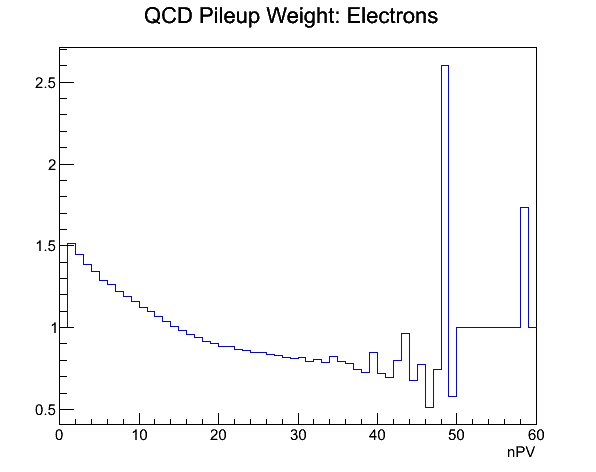
\includegraphics[width=\textwidth]{\figpath/Chapter5/QCD_PUWeights/QCD_PUWeights_fromTree_ele.png}
        \caption{}
        \label{fig:QCD_PUWeights_ele}
    \end{subfigure}

    \begin{subfigure}[t]{0.48\textwidth}
        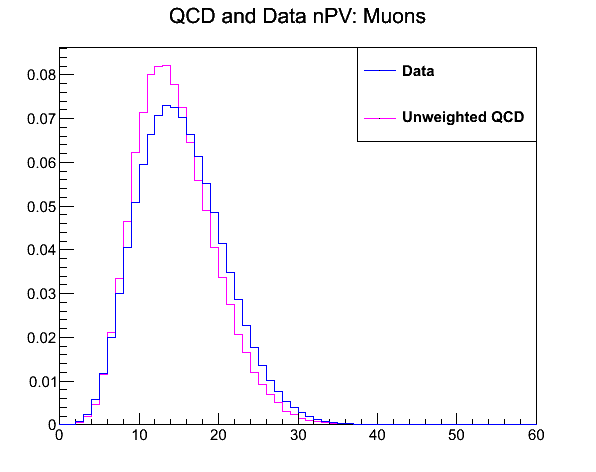
\includegraphics[width=\textwidth]{\figpath/Chapter5/QCD_PUWeights/QCDvData_nPV_mu.png}
        \caption{}
        \label{fig:QCDvData_nPV_mu}
    \end{subfigure}
    \begin{subfigure}[t]{0.48\textwidth}
        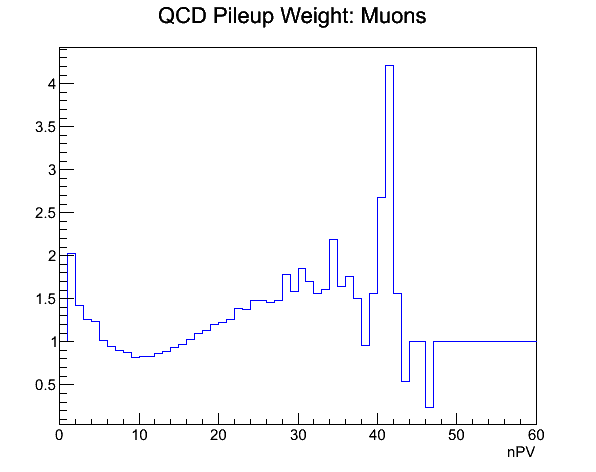
\includegraphics[width=\textwidth]{\figpath/Chapter5/QCD_PUWeights/QCD_PUWeights_fromTree_mu.png}
        \caption{}
        \label{fig:QCD_PUWeights_mu}
    \end{subfigure}
    \caption{Distribution of the number of primary vertices for data and QCD (a,c) and the associated weights (b,c). Figures (a) and (b) show the electron channel while figures (c) and (d) show the muon channel.}
    \label{fig:QCD_PUReweight}
\end{figure}

\subsection{CSV Reweighting}
Section~\ref{sec:btagging} introduced the criterion for tagging a jet as being produced by a \cPqb quark and the use of the Combined Secondary Vertex (CSV) discriminant.
The derivation of this discriminant is described in~\cite{Weiser:927399,BTV-12-001}.
This analysis relies heavily on the identification of \cPqb jets to veto the \ttbar background, so it is absolutely crucial that it behave the same in both data and MC and accurately describe the rate of observing a \cPqb jet.
\cite{CMS-AN-13-130} notes that the tagging efficiency in data is not the same as that in MC, so a correction to the CSV discriminant must be made.
The corrections described there both correct the rate of observing a jet in MC with a CSV value above a given threshold as well as the general shape of the CSV distribution.
If at the end of the procedure the shape of the data and MC distributions agree, then they will also properly assess the rate of events passing a given CSV threshold.

The method is based on calculating a scale factor for both heavy and light flavor quarks which is parameterized by the CSV value, jet \pt, and, in the case of light flavor quarks, jet $\eta$.
We first retrieve the truth level jet flavor in order to determine the correct category: \cPqb jet, \cPqc jet, or light flavor (anything else).
The \cPqc jets are given a flat scale factor of 1, meaning that there is no need to correct the CSV value for this flavor.
The \cPqb jet scale factors are divided into five \pt bins of \ptlt{40\gev}, \ptrange{40\gev}{60\gev}, \ptrange{60\gev}{100\gev}, \ptrange{100\gev}{160\gev}, and \ptgt{160\gev}.
The light flavor scale factors are divided into only three \pt bins of \ptlt{40\gev}, \ptrange{40\gev}{60\gev}, and \ptgt{60\gev}, but are also divided into three eta bins of \absetalt{0.8}, \absetaleqlt{0.8}{1.6}, and \absetaleqlt{1.6}{2.4}.
An individual scale factor is retrieved for each jet, which is then combined as in equation~\ref{eq:CSVWeight_SF_total} in order to create an event weight.
\begin{equation}\label{eq:CSVWeight_SF_total}
  SF_{\mathrm{total}}=\prod_{i}^{N_{\mathrm{jets}}}SF_{\mathrm{jet}_{i}}=SF_{\mathrm{jet}_{1}}{\cdot}SF_{\mathrm{jet}_{2}}{\cdot}...
\end{equation}
The CSV value for each jet is unchanged, but the event is weighted by $SF_{\mathrm{total}}$.

\subsection{\texorpdfstring{\ttbar}{TTbar} Reweighting}
\label{sec:topPt_reweighting}
Differential top-quark-pair analyses have shown that the shape of the \pt spectrum for top quarks is softer in data than predicted by simulation~\cite{Chatrchyan:2012saa,TopPtReweighting}.
Although it has been shown that NNLO predictions show reasonable agreement~\cite{Kidonakis2014}, this analysis must correct for the discrepancy in the \ttbar simulation.
Events are reweighted based on the \pt of the generator level \cPqt and \cPaqt in only the \ttbar simulation.
The weight $w_{\mathrm{TopPt}}$ is calculated as:
\begin{align}
  w_{\mathrm{TopPt}} ={}& \sqrt{SF_{\cPqt}{\cdot}SF_{\cPaqt}} \label{eq:TopPtWeight} \\
  SF\left(\ptsup{gen}\right) ={}& \exp\left(a+b\ptsup{gen}\right) \label{eq:TopPtSF}
\end{align}
with $a=0.156$ and $b=-0.00141$.
Fig.~\ref{fig:top_pt_weights} shows the distribution of weights for electron and muon events separately.
The bulk of the weights are centered around 1, indicating that no correction is necessary, with a long low side tail, indicating that a good fraction of events require the top \pt to be scaled down.
Some events do require that the top \pt be increased.

\begin{figure}[!hbt]
    \centering
    \begin{subfigure}[t]{0.48\textwidth}
      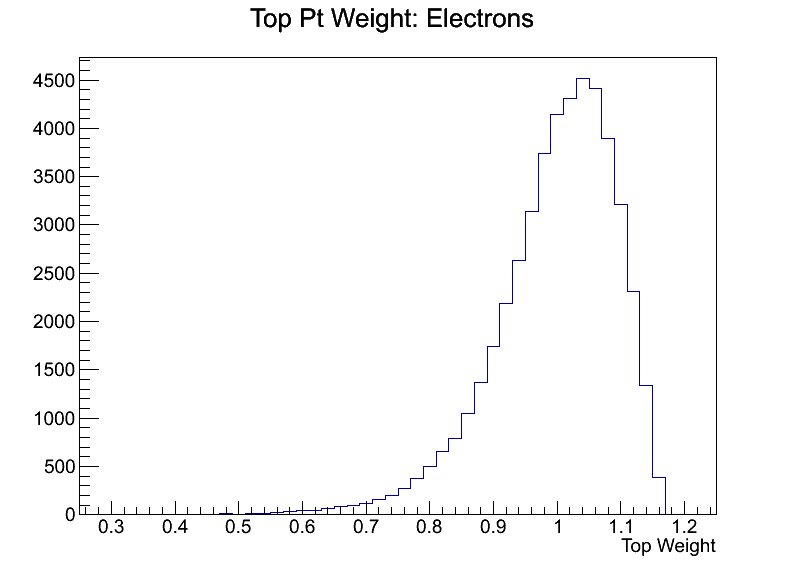
\includegraphics[width=\textwidth]{\figpath/Chapter5/top_weight_ele.png}
      \caption{}
      \label{fig:top_pt_weights_ele}
    \end{subfigure}
    \begin{subfigure}[t]{0.48\textwidth}
      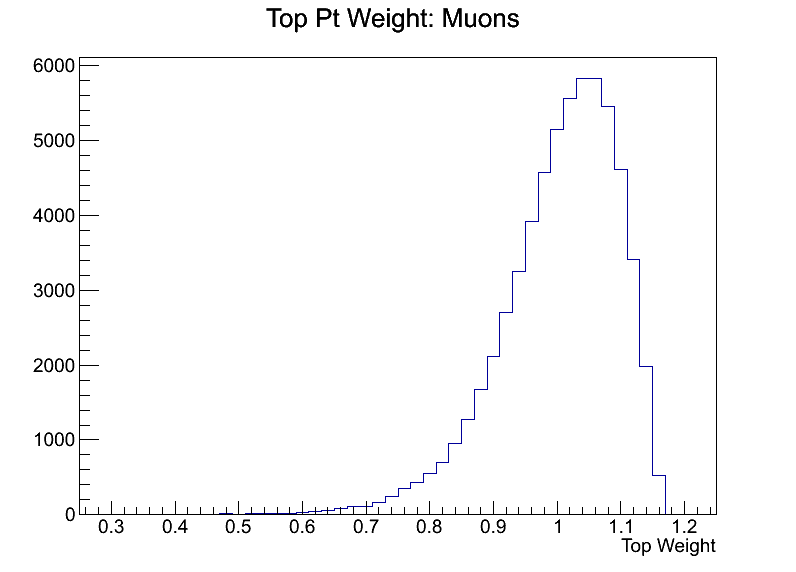
\includegraphics[width=\textwidth]{\figpath/Chapter5/top_weight_mu.png}
      \caption{}
      \label{fig:top_pt_weights_mu}
    \end{subfigure}
    \caption{Top \pt weight distributions for (a) electrons events and (b) muon events.}
    \label{fig:top_pt_weights}
\end{figure}

\subsection{\texorpdfstring{cos(theta$_l$)}{CosThetaL} Reweighting}
\label{sec:costhetal_reweighting}

A linear trend in the data to MC comparison of the \costhetal variable was discovered, indicating a mis-modeling problem in the simulation.
\costhetal is one of the angular variables involved in the \WW system and is the cosine of the angle between the daughter lepton and the \WW decay plane, which corresponds to $\cos\left(\theta_{2}\right)$ in fig.~\ref{fig:XWWDecayAngles}.
Fig.~\ref{fig:cos_theta_l_preweight_signal} shows this trend in the two jet bin, though the trend is the same in the other jet bins.

\begin{figure}[!hbt]
    \centering
    \begin{subfigure}[t]{0.48\textwidth}
      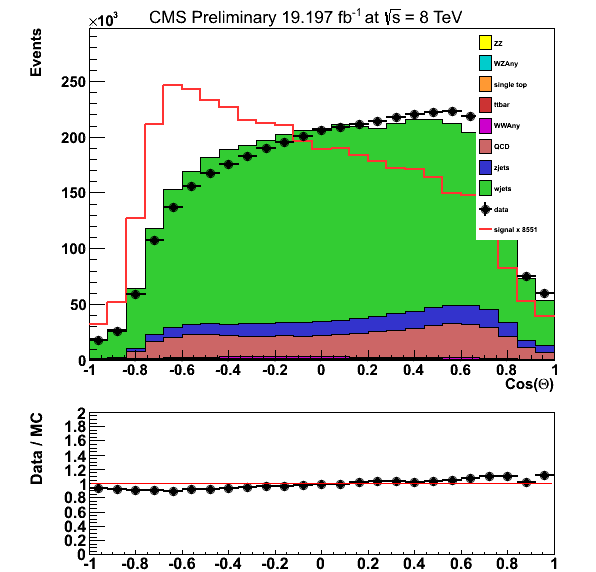
\includegraphics[width=\textwidth]{\figpath/Chapter5/CosThetaPlots/CosThetaL_2Jets_preWeight.png}
      \caption{}
      \label{fig:cos_theta_l_preweight_signal}
    \end{subfigure}
    \begin{subfigure}[t]{0.48\textwidth}
      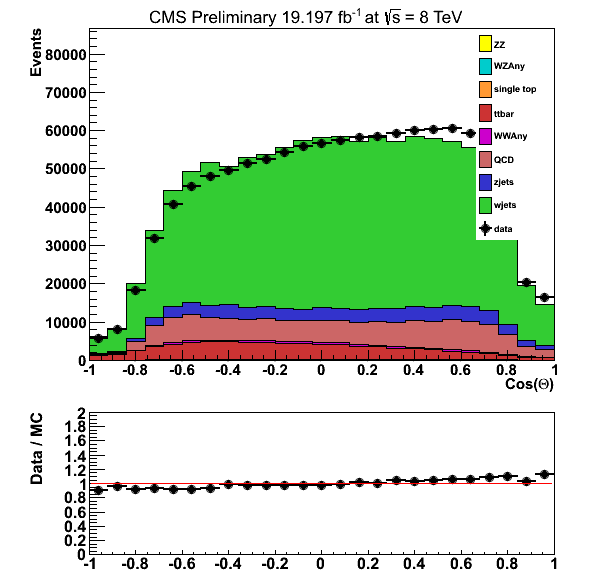
\includegraphics[width=\textwidth]{\figpath/Chapter5/CosThetaPlots/CosThetaL_2Jets_BTagRegion.png}
      \caption{}
      \label{fig:cos_theta_l_preweight_1btag}
    \end{subfigure}
    \caption{Distribution of \costhetal for data and MC in the two jet bin for (a) the signal region and (b) the one b-tag region. The top of each figure shows the data and MC expectations while the bottom shows their ratio with a clear linear trend.}
    \label{fig:cos_theta_l_preweight}
\end{figure}

We correct for the trend in the \Wjets MC as this is the biggest background and correcting it will improve the overall agreement.
We create the corrections in the one b-tag control region shown in fig.~\ref{fig:cos_theta_l_preweight_1btag} so as to not bias our backgrounds in the signal region.
It's clear from fig.~\ref{fig:cos_theta_l_preweight} that the trend in the one b-tag region is the same as the trend in the signal region.
Although the regions are similar, the \ttbar MC plays a much larger role in the control region because it contains two real \cPqb jets.
Therefore we subtract the expected \ttbar yield from the data before creating the weights.
The new weights shown in fig.~\ref{fig:cos_theta_l_weight} are combined multiplicatively with the pileup and CSV weights for the \Wjets sample.
The corrected distribution is shown in fig.~\ref{fig:cos_theta_l_corrected} where it is clear that the trend has been removed.

\begin{figure}[!hbt]
    \centering
    \begin{subfigure}[t]{0.48\textwidth}
      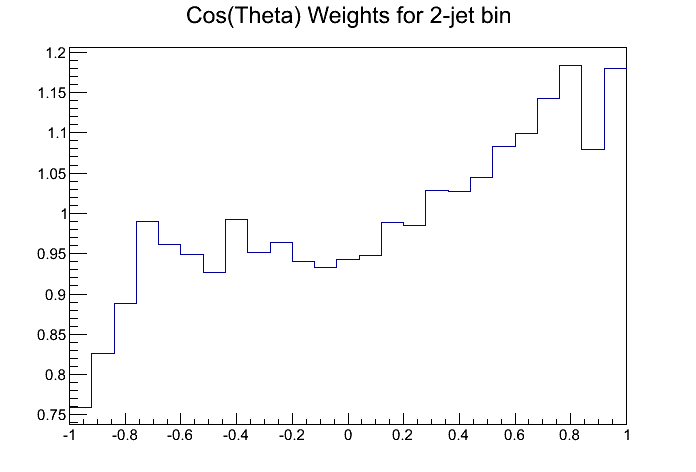
\includegraphics[width=\textwidth]{\figpath/Chapter5/CosThetaPlots/CosThetaWeight_2Jets_lep_ControlRegion.png}
      \caption{}
      \label{fig:cos_theta_l_weight}
    \end{subfigure}
    \begin{subfigure}[t]{0.48\textwidth}
      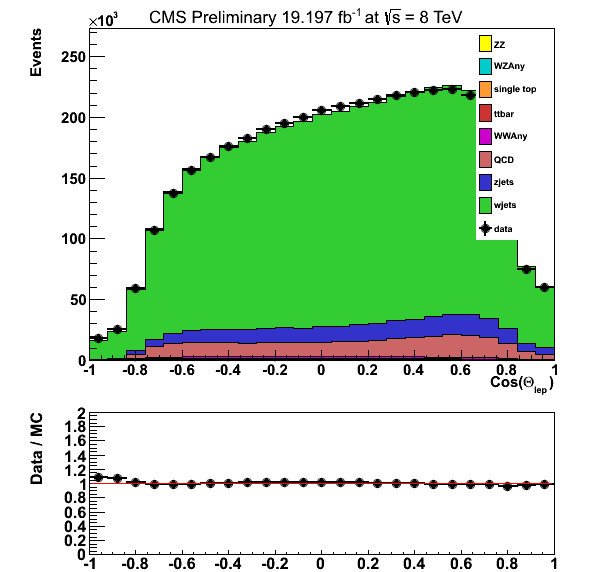
\includegraphics[width=\textwidth]{\figpath/Chapter5/CosThetaPlots/CosThetaL_2Jets_Corrected.png}
      \caption{}
      \label{fig:cos_theta_l_corrected}
    \end{subfigure}
    \caption{(a) Weights created in the one b-tag control region used to correct the \costhetal mis-modeling. (b) \costhetal distribution in the signal region after applying the weights.}
    \label{fig:cos_theta_l_postweight}
\end{figure}

\subsection{QCD Reweighting}
\label{sec:QCD_reweighting}

As stated in section~\ref{sec:QCD_data-driven_sample}, the QCD sample is obtained by selecting on anti-isolated leptons, as opposed to the isolated signal selection.
Although these regions are similar kinematically, the ratio of the number of events in the signal region to the number of events in the anti-isolated region changes significantly as a function of $\eta$.
This effect was first noticed in MC, which was used to check the anti-isolation procedure despite its limited statistics in the low \pthat-binned samples.
Fig.~\ref{fig:SfVsEtaMC} shows the suspect ratio as a function of $\eta$ in the different QCD \pthat bins.
The effect seems to be particularly large in the endcap regions (\absetagt{1.3}).
A weighting procedure is necessary to make sure that the expected yield as a function of $\eta$ for the data-driven QCD sample is correct when used in the signal region.

\begin{figure}[!hbt]
    \centering
    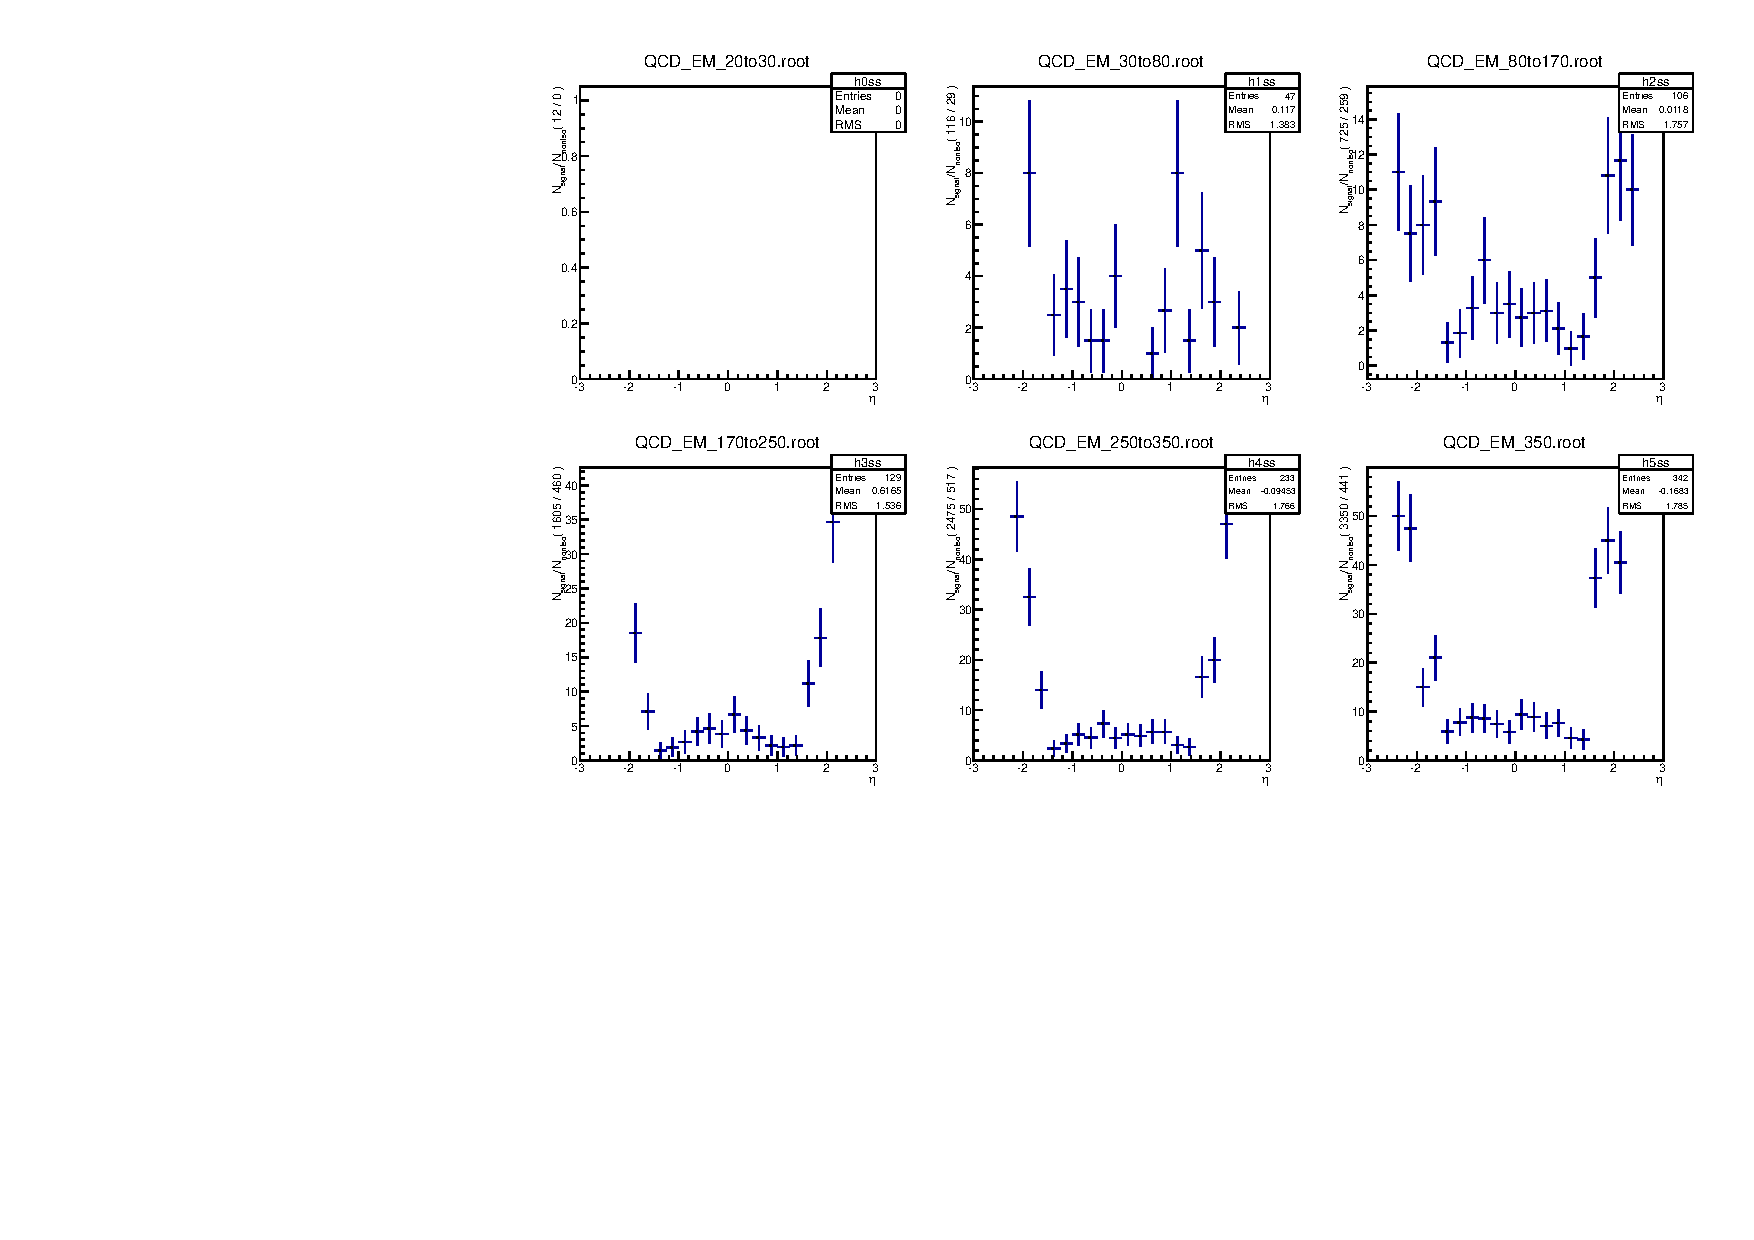
\includegraphics[width=\textwidth]{\figpath/Chapter5/QCD_EtaWeights/SfVsEtaMC.pdf}
    \caption{The ratio of the number of events in the signal region to the number of events in the anti-isolated region for six QCD \pthat bins. The total number of events in the two regions is shown in parentheses along the $y$-axis. The first plot is empty due to the low number of MC events which pass the selection criteria.}
    \label{fig:SfVsEtaMC}
\end{figure}

To derive the weights we use the one jet control region separated into 13 (12) bins of lepton $|eta|$ for the electron (muon) channel.
We want to find the scale factor $S_{\mathrm{QCD}}$ such that:
\begin{equation}
  N_{\mathrm{anti-isolated}}^{\mathrm{QCD}}\left(\eta\right)S_{\mathrm{QCD}}\left(\eta\right)=N_{\text{signal region}}^{\mathrm{QCD}}\left(\eta\right),
\end{equation}
where $N_{\mathrm{anti-isolated}}^{\mathrm{QCD}}$ and $N_{\text{signal region}}^{\mathrm{QCD}}$ represent the number of events in the anti-isolated and signal regions, respectively, given the same luminosity in both.
In order to determine the scale factor needed to to modify the QCD contribution in each bin, we perform a fit to the data using the \ETslash distribution.
The QCD and \Wjets contributions are allowed to float while the contributions from all of the other backgrounds are fixed to their SM expectations.
The \ETslash distributions post-fitting as well as the $\chi^{2}/NDF$ for all of the fits are shown in fig.~\ref{fig:AllMetFits_control6_electron}.
The fit returns both the scale factor $S_{\mathrm{QCD}}$ as well as a scale factor for the \Wjets, $S_{\Wjets}$, which are shown in fig.~\ref{fig:SfVsEta_control6_electron}.
The shape of the weights follows very closely the shape of the ratio in MC from fig.~\ref{fig:SfVsEtaMC}, which is a very good indication that we are indeed correcting for the intended effect.
The same procedure is performed for the muon events, yielding the weights shown in fig.~\ref{fig:SfVsEta_control6_muon}.
Note that the absolute value of the scale factors is not what matters, only their relative values, as the sample will undergo an additional normalization in order to obtain the correct yield.

\begin{figure}[!hbt]
    \centering
    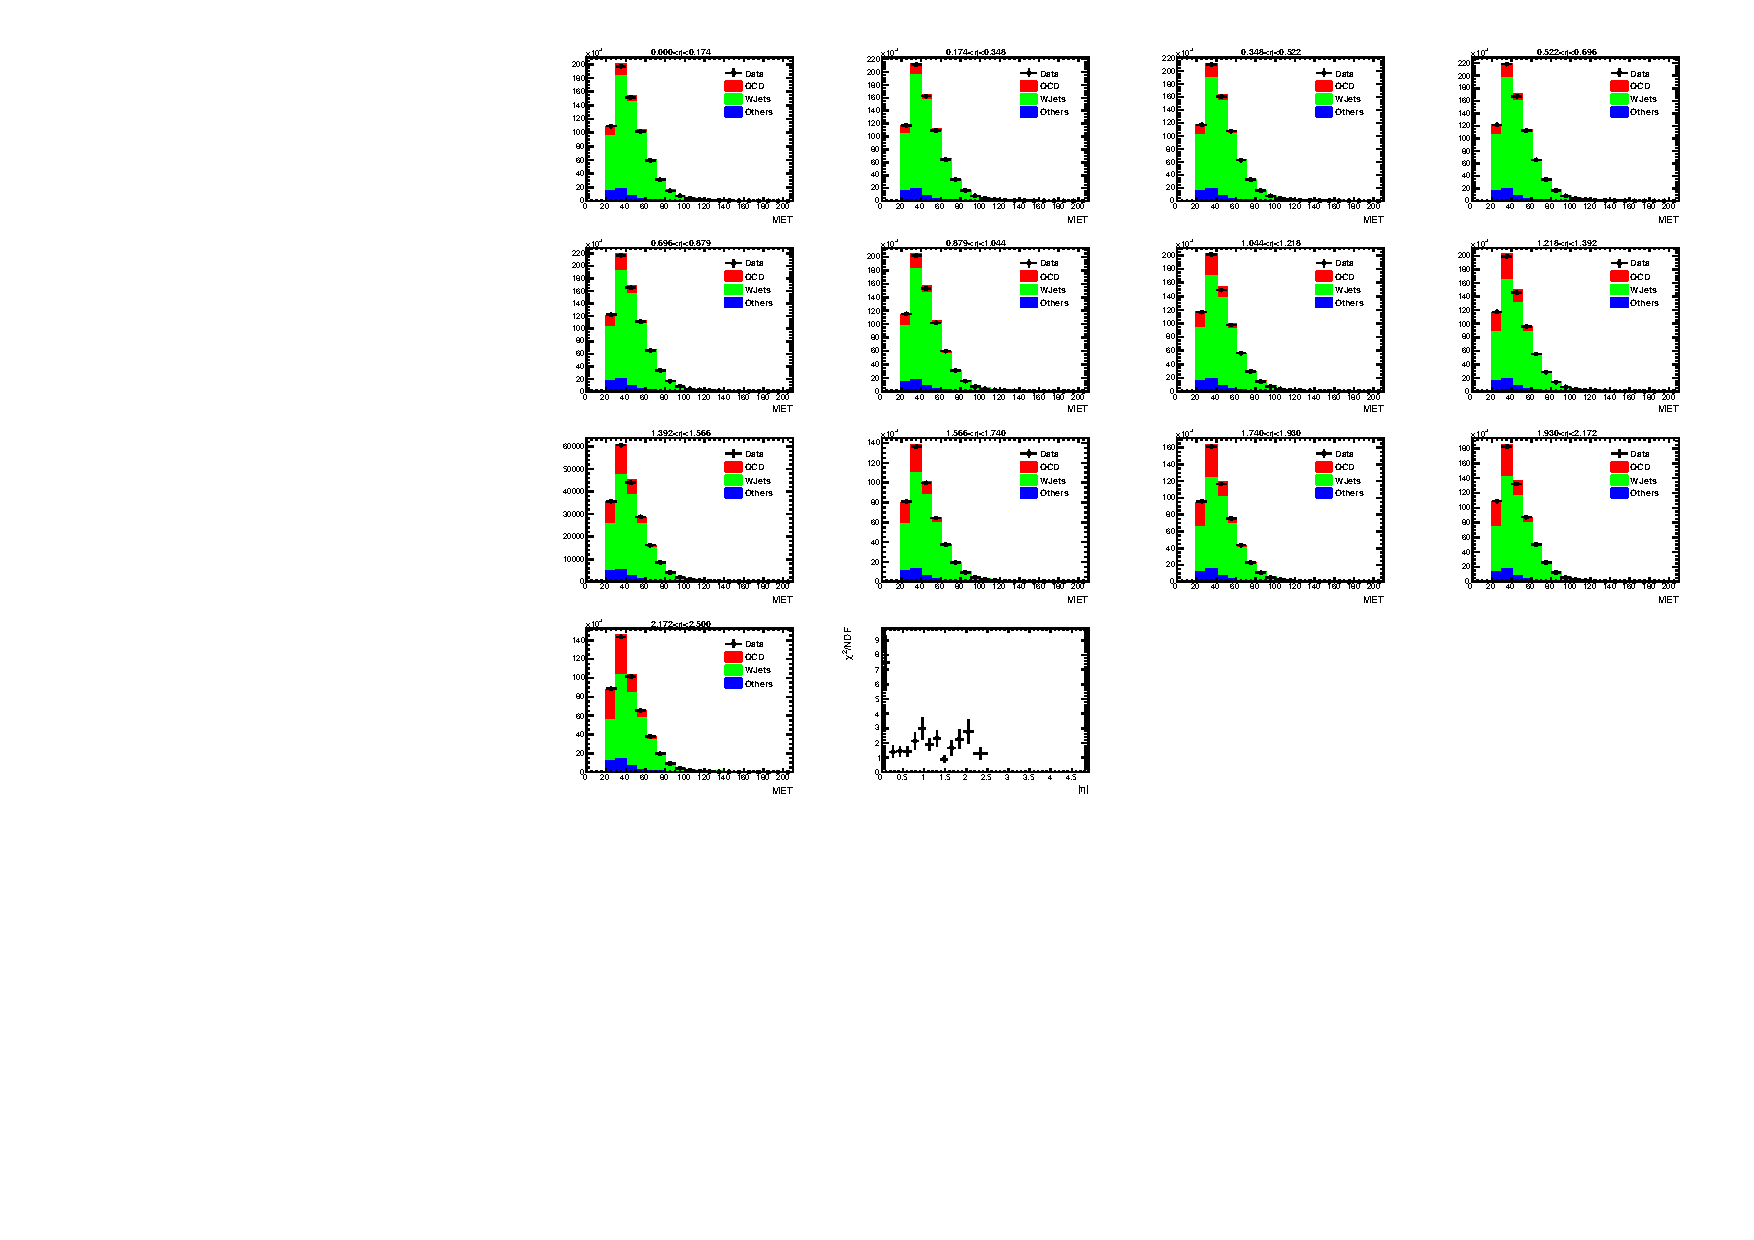
\includegraphics[width=\textwidth]{\figpath/Chapter5/QCD_EtaWeights/AllMetFits_control6_electron.pdf}
    \caption{The \ETslash distributions used to derive the QCD weights in the 13 different bins of lepton $|\eta|$ after the fitting the QCD (red) and \Wjets (green) contributions to the data (black markers). The contribution from the other SM processes (blue) is held fixed to their SM expectation. The last pad in the plot show the $\chi^{2}/NDF$ of the fits.}
    \label{fig:AllMetFits_control6_electron}
\end{figure}

\begin{figure}[!hbt]
    \centering
    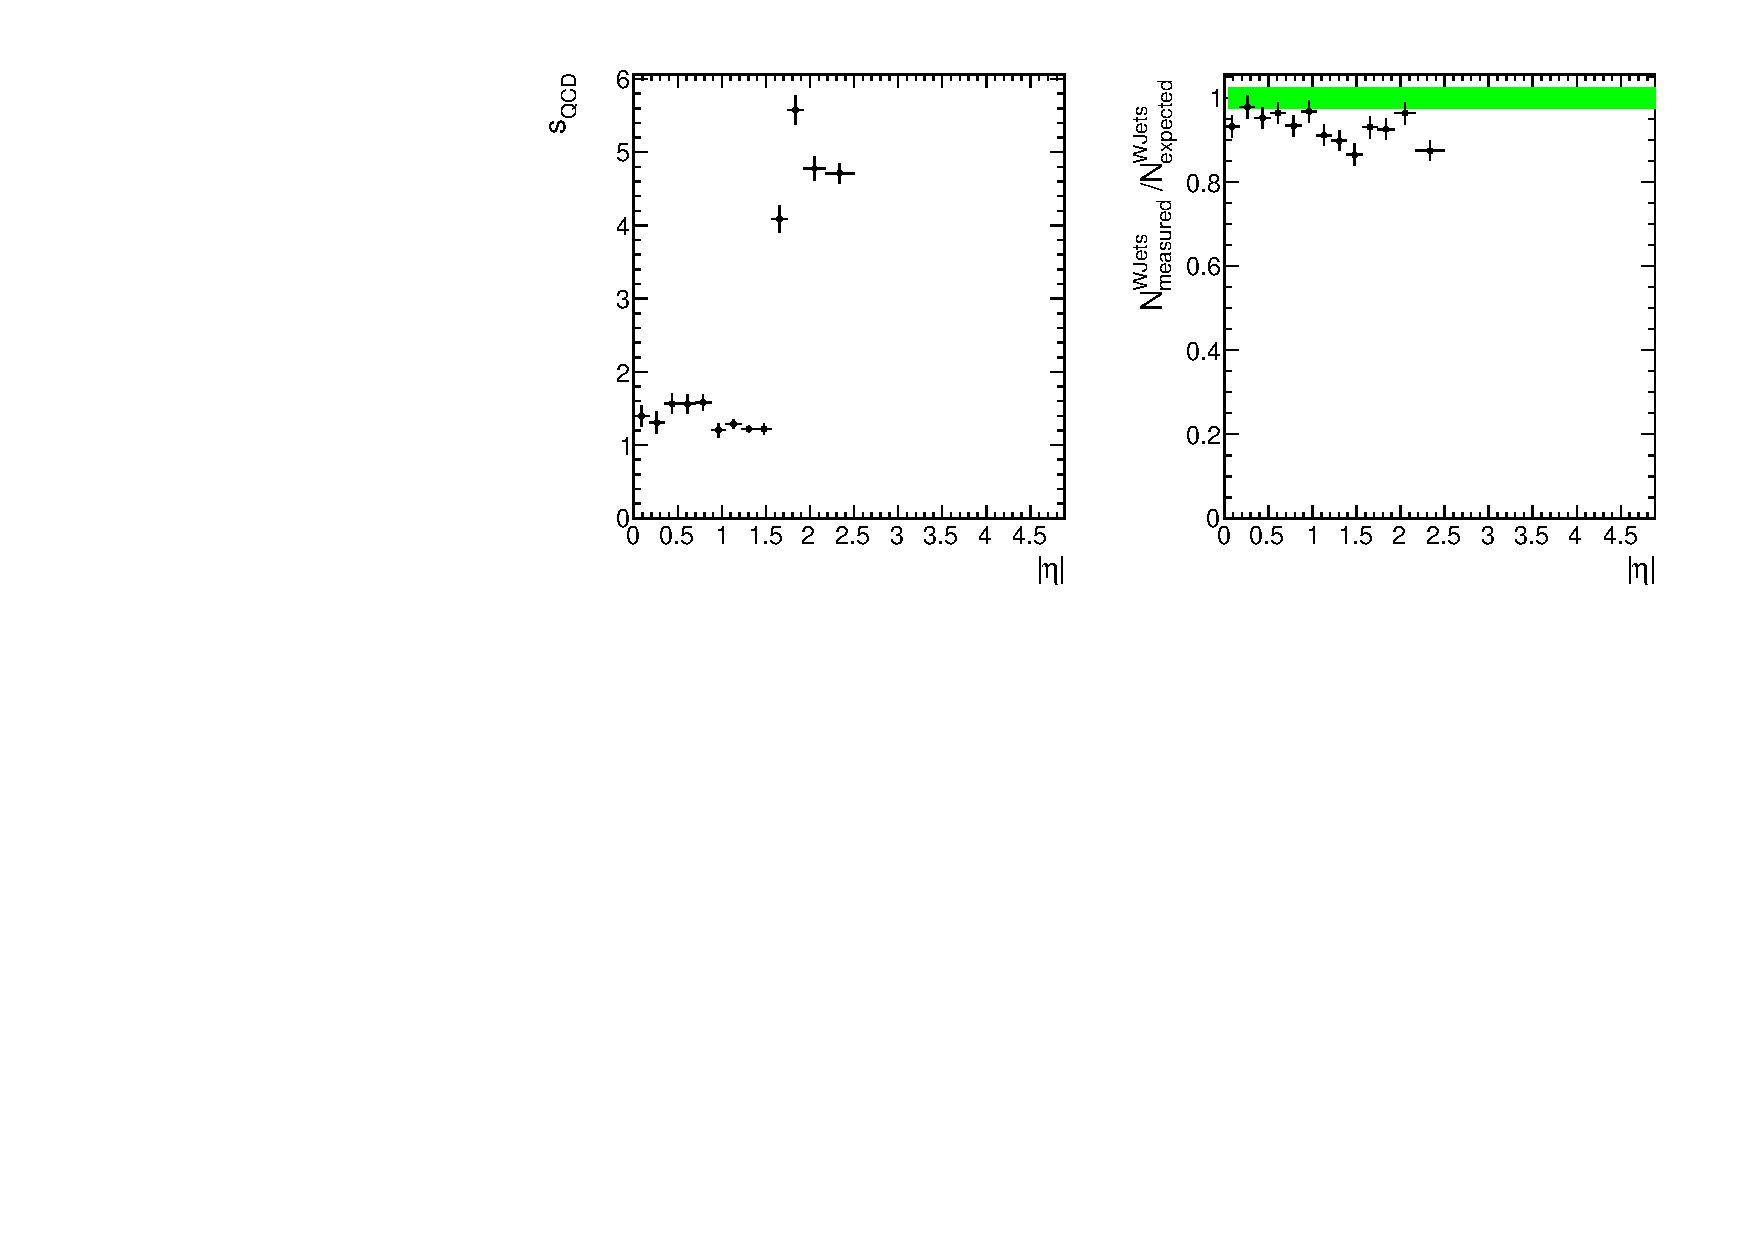
\includegraphics[width=\textwidth]{\figpath/Chapter5/QCD_EtaWeights/SfVsEta_control6_electron.pdf}
    \caption{$S_{\mathrm{QCD}}$ (left) and $S_{\Wjets}$ (right) scale factors as a function of lepton $|\eta|$ derived in the electron channel for the one jet bin. The green band indicates the uncertainty on the \Wjets expectation due to the theoretical uncertainty in the SM cross section.}
    \label{fig:SfVsEta_control6_electron}
\end{figure}

\begin{figure}[!hbt]
    \centering
    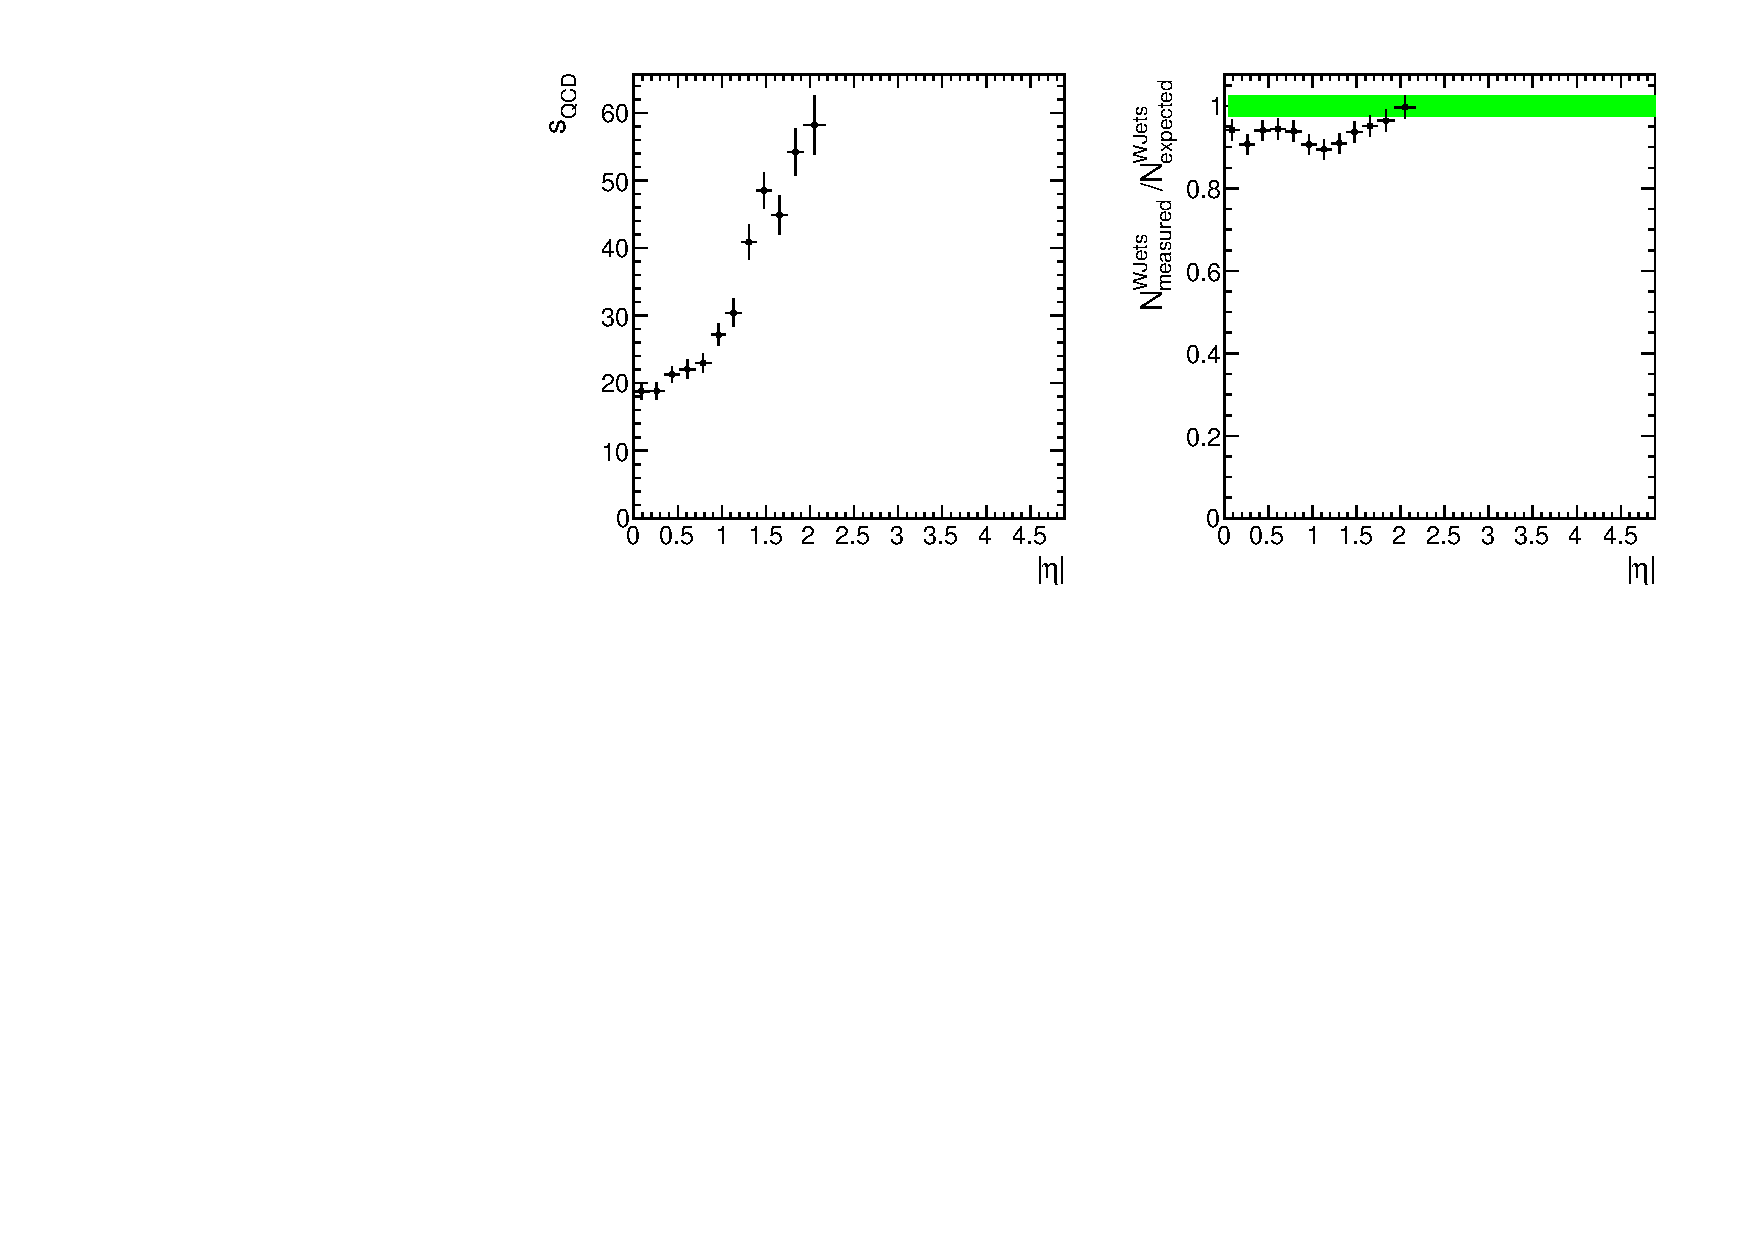
\includegraphics[width=\textwidth]{\figpath/Chapter5/QCD_EtaWeights/SfVsEta_control6_muon.pdf}
    \caption{$S_{\mathrm{QCD}}$ (left) and $S_{\Wjets}$ (right) scale factors as a function of lepton $|\eta|$ derived in the muon channel for the one jet bin. The green band indicates the uncertainty on the \Wjets expectation due to the theoretical uncertainty in the SM cross section.}
    \label{fig:SfVsEta_control6_muon}
\end{figure}

As an additional cross check, the same procedure was done to the $\geqslant$2 jets bin to see if the distribution of weights was similar to that of the control region.
From figs.~\ref{fig:AllMetFits_signal_electron} and~\ref{fig:SfVsEta_signal_electron} we see that the procedure, done on the signal region, does indeed return similar scale factors to those found in the one jet control region.
This gives us high confidence that the scale factors from the one jet bin will correct the shape of the QCD distributions in the signal region.

\begin{figure}[!hbt]
    \centering
    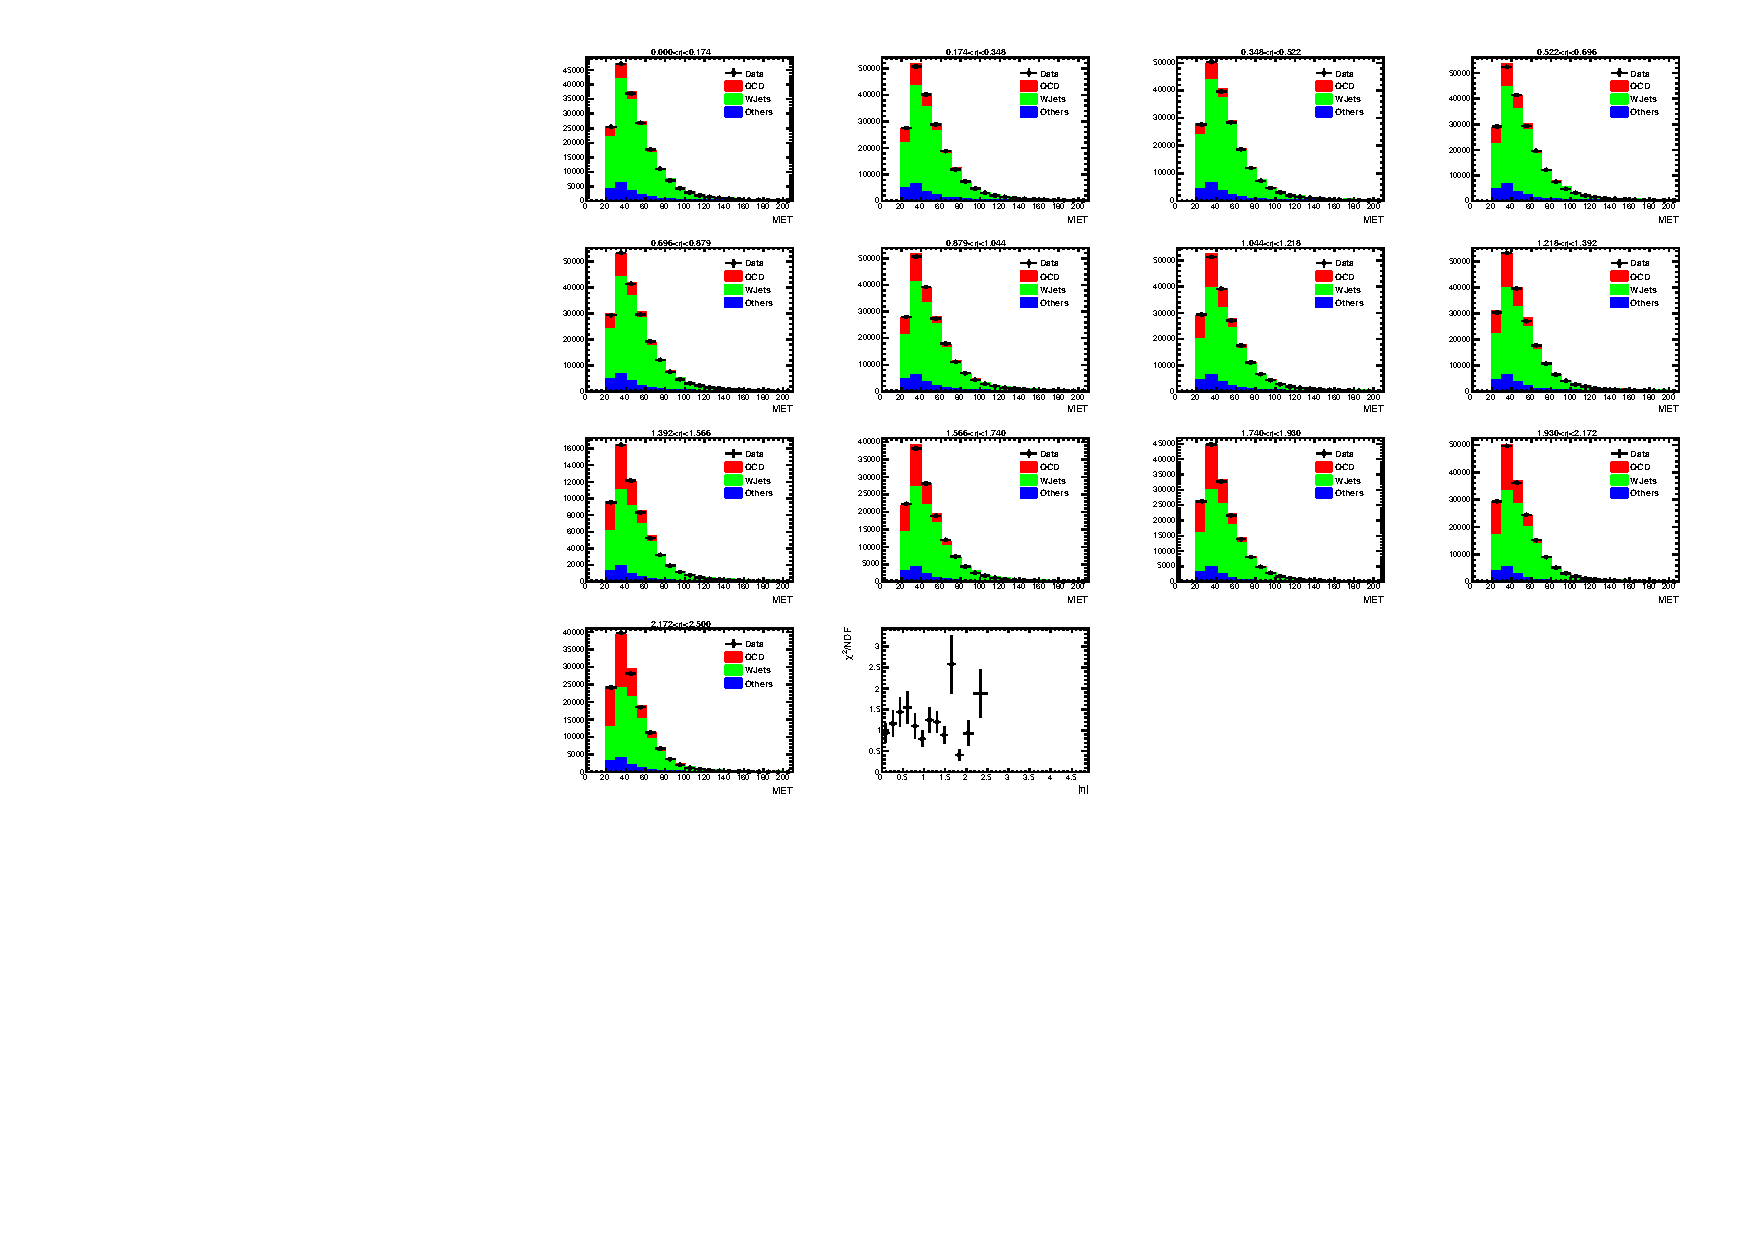
\includegraphics[width=\textwidth]{\figpath/Chapter5/QCD_EtaWeights/AllMetFits_signal_electron.pdf}
    \caption{The \ETslash distributions in the $\geqslant$2 jet bin used to derive the QCD weights in the 13 different bins of lepton $|\eta|$ after the fitting the QCD (red) and \Wjets (green) contributions to the data (black markers). The contribution from the other SM processes (blue) is held fixed to their SM expectation. The last pad in the plot show the $\chi^{2}/NDF$ of the fits.}
    \label{fig:AllMetFits_signal_electron}
\end{figure}

\begin{figure}[!hbt]
    \centering
    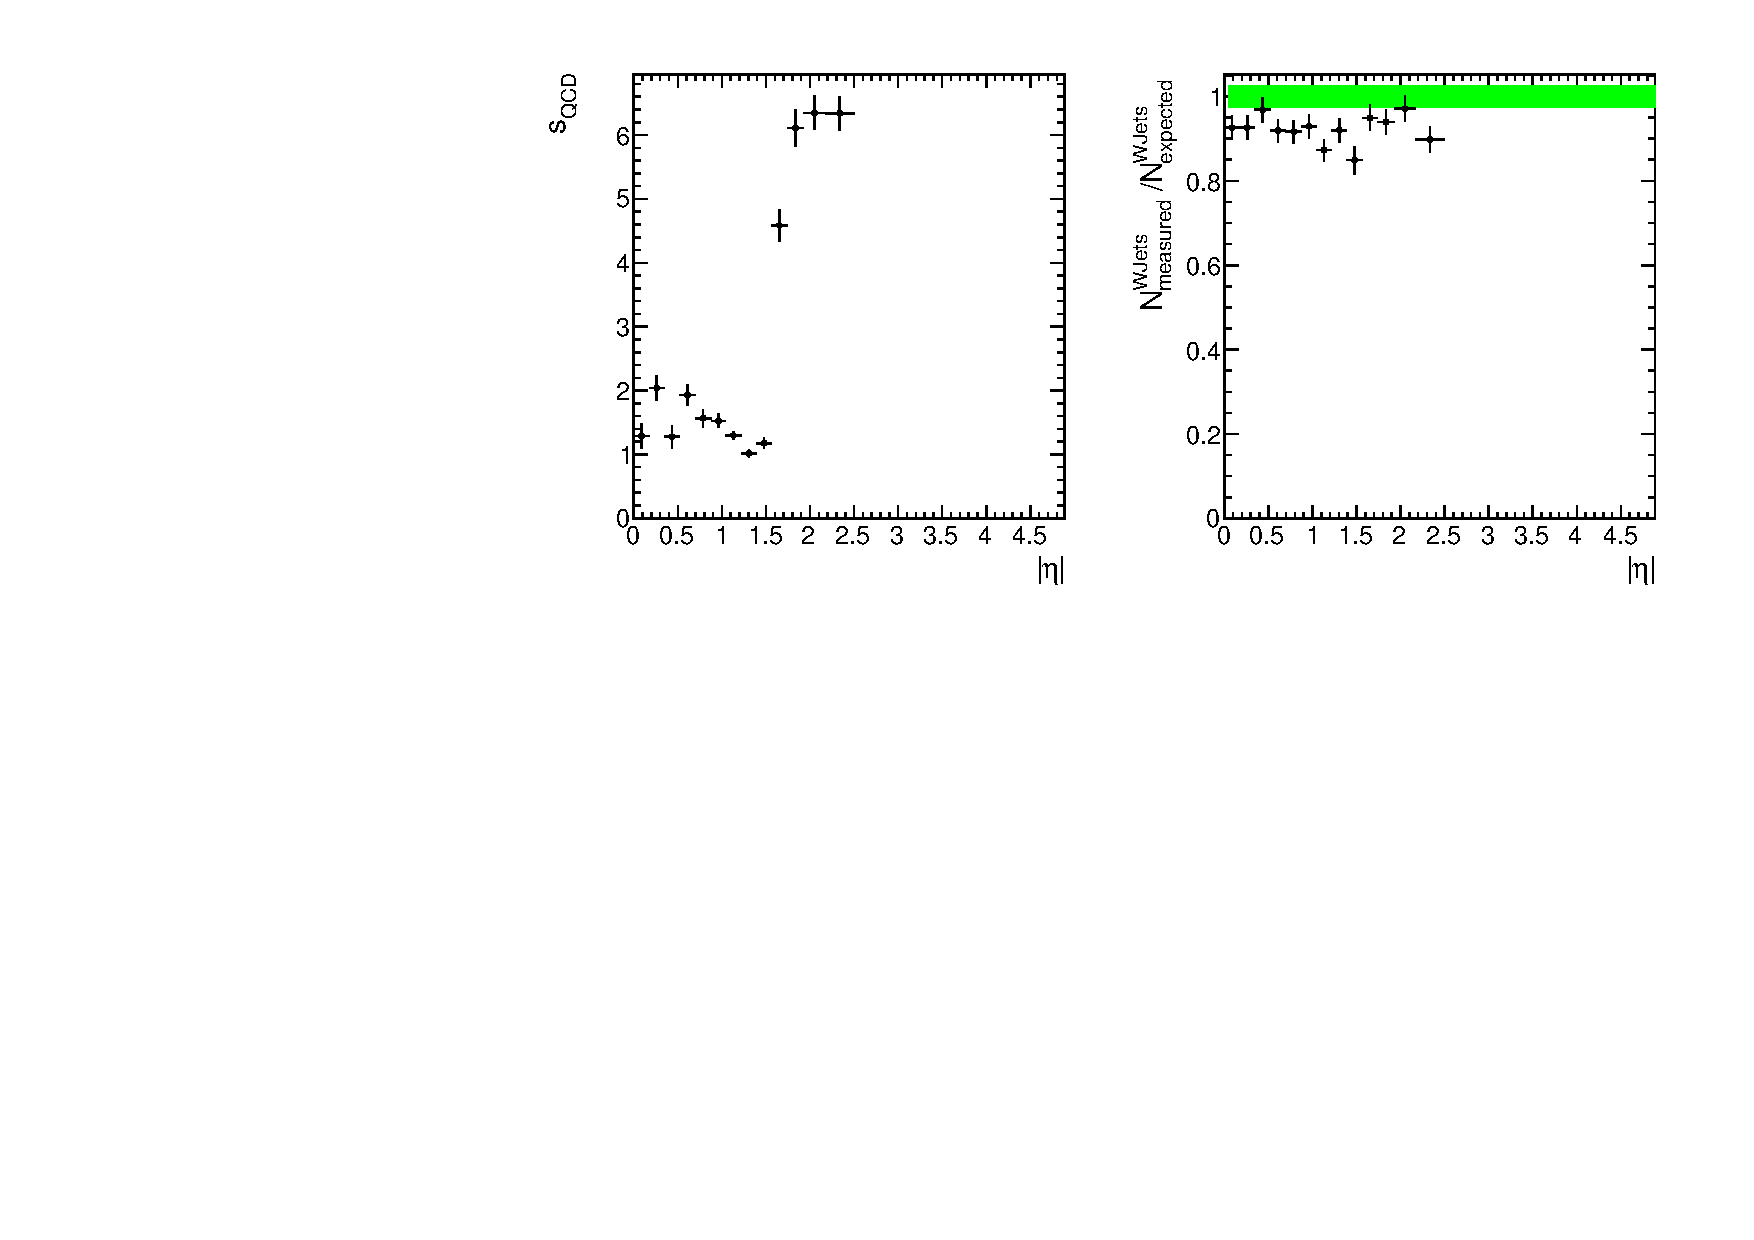
\includegraphics[width=\textwidth]{\figpath/Chapter5/QCD_EtaWeights/SfVsEta_signal_electron.pdf}
    \caption{$S_{\mathrm{QCD}}$ (left) and $S_{\Wjets}$ (right) scale factors as a function of lepton $|\eta|$ derived in the electron channel for the $\geqslant$2 jet bin. The green band indicates the uncertainty on the \Wjets expectation due to the theoretical uncertainty in the SM cross section.}
    \label{fig:SfVsEta_signal_electron}
\end{figure}

The right plot of fig.~\ref{fig:SfVsEta_signal_electron} shows that the \Wjets normalization also needs to be measured as a fit to the ratio of measured events and expected events yields a value of $0.953\pm0.008$, which is not consistent with the 2.56\% error on the theoretical cross section.
To find the correct \Wjets and QCD normalizations a two component fit to the \ETslash distribution of the data is used, allowing only the \Wjets and QCD fractions to float.
The expected yields of the other SM backgrounds are held constant during the fit.
A Gaussian constraint is imposed on the \Wjets scale factor because its theoretical cross section uncertainty is known.
The derived scale factors are shown in table~\ref{tab:WJet_QCD_ScaleFactors}.

\begin{table}[hbtp]\footnotesize
\centering
\begin{tabular}{l l l}
\hline
Lepton Category & \Wjets SF & QCD SF \\
\hline
Electron & $1.04515\pm0.00509474$ & $0.248858\pm0.0131115$ \\
Muon     & $0.969517\pm0.00442517$ & $0.145418\pm0.00669525$ \\
\hline
\end{tabular}
\caption{\Wjets and QCD scale factors as derived from a two component fit to the \ETslash distribution.}
\label{tab:WJet_QCD_ScaleFactors}
\end{table}

\section{Data-to-MC Comparisons \& Yields}

After applying all of the object and event selections, object corrections, and event weights we can now look at the expected yields for the simulated signals and backgrounds.
Table~\ref{tab:yields_KinMEBDT} shows the event yields for our signal selection separated by jet bin, but combining the electron and muon categories.
Table~\ref{tab:percent_yields_KinMEBDT}, on the other hand, shows the percentage yields where the numbers from table~\ref{tab:yields_KinMEBDT} have been normalized to the sum of the events in background and signal sections.
In both tables, Higgs events where the Higgs boson does not decay to two \W bosons are referred to as 'volunteer signal'.
This is in contrast to true \HWW events, which we sometimes refer to as 'true signal'.
Both of these categories are normalized to the \HWW yields in order to be able to compare the volunteer signal contamination to the true signal.

\begin{sidewaystable}[htbp]
\centering
\begin{tabular}{lccc} \hline
\textbf{Process} & \textbf{2 Jets} & \textbf{3 Jets} & \textbf{$\geqslant$4 Jets}\\ \hline
Diboson & $46495.97\pm78.55$ & $15049.18\pm44.70$ & $4150.48\pm23.47$ \\
\Wjets & $3446003.06\pm6434.30$ & $756463.35\pm3008.63$ & $189815.29\pm1515.40$ \\
\Zjets & $270460.62\pm822.24$ & $69061.73\pm415.90$ & $19829.24\pm222.71$ \\
\ttbar & $22452.06\pm142.85$ & $27902.44\pm160.86$ & $31218.33\pm170.54$ \\
Single \cPqt & $16587.13\pm84.31$ & $7193.89\pm59.29$ & $3068.60\pm40.25$ \\
Multijet & $275465.33\pm952.52$ & $74168.89\pm504.39$ & $22109.53\pm282.94$ \\\hline
\rowcolor{mygray}
Total Background & $4077464.17\pm6558.75$ & $949839.48\pm3083.93$ & $270191.47\pm1567.59$ \\\hline
ggH, \HWW \MH=125\gev & $552.09\pm1.92$ & $211.15\pm1.19$ & $79.51\pm0.73$ \\
qqH, \HWW \MH=125\gev & $106.60\pm0.56$ & $52.66\pm0.39$ & $17.51\pm0.23$ \\
WH\_ZH\_TTH, \HWW \MH=125\gev & $136.20\pm2.22$ & $84.35\pm1.75$ & $42.32\pm1.22$ \\\hline
\rowcolor{mygray}
Total \HWW & $794.89\pm2.99$ & $348.16\pm2.15$ & $139.34\pm1.44$ \\\hline
WH\_ZH\_TTH, \HZZ \MH=125\gev & $10.30\pm0.17$ & $5.30\pm0.12$ & $2.35\pm0.08$ \\
WH, \Hbb \MH=125\gev & $45.34\pm0.40$ & $14.22\pm0.23$ & $3.86\pm0.12$ \\
\ttH, \Hbb \MH=125\gev & $0.59\pm0.03$ & $1.33\pm0.05$ & $3.77\pm0.09$ \\\hline
\rowcolor{mygray}
Total Volunteer Signal & $56.23\pm0.44$ & $20.85\pm0.26$ & $9.98\pm0.17$ \\\hline
Signal \textsubscript{\HWW}/Bkg & 0.000195 & 0.000367 & 0.000516 \\
Signal \textsubscript{\HWW}/$\sqrt{\text{Bkg}}$ & 0.394 & 0.357 & 0.268 \\\hline
\rowcolor{mygray}
Data & $4057594$ & $953513$ & $272713$ \\\hline
\end{tabular}
\caption{Expected yields for both the electron and muon categories when normalized to the SM cross sections and collected luminosity. The table is broken up into three sections; the top section contains all of the background processes, the middle section shows the \HWW contributions, and the bottom section shows the other Higgs processes that could mimic our final state, but do not originate from a \HWW process. This table contains the yields for the zero b-tag category. Only statistical uncertainties are shown.}
\label{tab:yields_KinMEBDT}
\end{sidewaystable}

\begin{table}[htbp]
\centering
\begin{tabular}{lccc} \hline
\textbf{Process} & \textbf{2 Jets} & \textbf{3 Jets} & \textbf{$\geqslant$4 Jets}\\ \hline
Diboson & 0.011 & 0.016 & 0.015 \\
\rowcolor{green}
\Wjets & 0.845 & 0.796 & 0.703 \\
\Zjets & 0.066 & 0.073 & 0.073 \\
\ttbar & 0.006 & 0.029 & 0.116 \\
Single \cPqt & 0.004 & 0.008 & 0.011 \\
Multijet & 0.068 & 0.078 & 0.082 \\\hline
\rowcolor{mygray}
Total Background & 1.000 & 1.000 & 1.000 \\\hline
ggH, \HWW \MH=125\gev & 0.695 & 0.606 & 0.571 \\
qqH, \HWW \MH=125\gev & 0.134 & 0.151 & 0.126 \\
WH\_ZH\_TTH, \HWW \MH=125\gev & 0.171 & 0.242 & 0.304 \\\hline
\rowcolor{mygray}
Total \HWW & 1.000 & 1.000 & 1.000 \\\hline
WH\_ZH\_TTH, \HZZ \MH=125\gev & 0.013 & 0.015 & 0.017 \\
WH, \Hbb \MH=125\gev & 0.057 & 0.041 & 0.028 \\
\ttH, \Hbb \MH=125\gev & 0.001 & 0.004 & 0.027 \\\hline
\rowcolor{mygray}
Total Volunteer/Total \HWW & 0.071 & 0.060 & 0.072 \\\hline
\end{tabular}
\caption{Expected percent yields for both the electron and muon categories separated by jet bin. The background samples are normalized by the total background, while the \HWW and volunteer signal samples are normalized by the \HWW total. The Dominant background in all jet bins, \Wjets, is highlighted in green. This table contains the percent yields for the zero b-tag category.}
\label{tab:percent_yields_KinMEBDT}
\end{table}

It is clear from these tables that the dominant background for all jet bins is \Wjets.
Its expected yield is by far much larger than all of the other backgrounds.
From table~\ref{tab:percent_yields_KinMEBDT} one can also see that the sum of the volunteer signal is at most 7\% of the \HWW signal, which means the b-tag cut is keeping the non-\HWW contamination to a minimum.
If the b-tag cut was not used the \ttbar background would become much more significant, even becoming the dominant background in the $\geqslant$4 jet bin.
Additionally, the volunteer signal would become as high as 87\% of the \HWW signal, which means that there would be a lot of overlap between this analysis and other CMS analyses.

\section{Multivariate Analysis}

One of the problems of past analyses, such as cut-and-count experiments, is that they ignore the additional information that comes from using the many correlated bins of a shape analysis.
By doing a cut-and-count experiment across many bins an analysis is able to gain in discrimination power.
That being said, it would be wasteful and suboptimal to use a single discriminating kinematic distribution, which means the discrimination power of the unused variables is missed.
This analysis uses the output of a boosted decision tree (BDT) classifier as the template used for limit setting, choosing to combine the discrimination power of several kinematic variables.
This type of multivariate analysis (MVA) is useful in quantifying the separation of the signal samples (\HWW) from the background samples.

\subsection{Boosted Decision Tree}

Multivariate techniques are used to model the dependence of one or more target variables on a set of input variables.
Boosted decision trees are a more robust alternative to artificial neural networks and were first introduced to the high energy physics (HEP) community by the MiniBooNE collaboration~\cite{Roe:2004na}.
This machine learning (ML) technique has since been used countless times throughout the HEP community.
This analysis makes use of the BDT algorithm implemented in the ROOT TMVA package~\cite{1742-6596-219-3-032057}.
The key ingredient here is the boosting technique, which helps to mitigate the problem of ``overtraining,'' which is common to ML algorithms, and increases the overall performance of the algorithm~\cite{Hocker:2007ht}.
The issue with overtraining is that the output of the ML algorithm becomes overly dependent on the multivariate inputs.
In other words this means that a small change in the input variable $x{\rightarrow}x+\delta{x}$ can cause a large change in the output of the algorithm $f\left(x+\delta{x}\right)-f\left(x\right)\gg\epsilon$.
The ML algorithm may be picking up on minute changes in the simulation or statistical fluctuations, both of which are not true features of the target classification.
While these jumps may seem to indicate a higher amount of discrimination power in the training sample, they are not indicative of the underlying physics being modeled and must be suppressed.
The BDT algorithm train many weak decision trees, which are then combined using the namesake ``boosting algorithm.''
This algorithm ``boosts'' the events that are misclassified in the previous tree so that each successive generation of tree contains fewer misclassified events.
Some of the benefits of boosting are that weak or less discriminating input variables will have a reduced impact and that many input variables can be included to improve the overall classification performance.
This section will describe the general process of training of a BDT classifier while the subsequent sections will explain how the BDTs were trained for this analysis.

A decision tree is a binary tree structure made up of nodes which are meant to provide higher purity samples of signal and background at each subsequent layer of the tree.
A set of input variables is chosen by the analyzer before the start of the training sequence.
The higher purity is achieved by placing a cut on the single input variable which will achieve the best separation (highest purity) at any given node.
This can be thought of as each node creating a boundary $t\left(x\right)$ in multi-dimensional space and estimating the likelihood ratio $\frac{\mathcal{L}\left(t|S\right)}{\mathcal{L}\left(t|B\right)}$ in a small portion of that space.
The input variables should be chosen for their discrimination power, which can be quantified at each stage of the tree as $S/\left(S+B\right)$.
The signal purity $P$, on the other hand, is defined at every node as the number of signal events divided by the total number of events in the sample, both signal and background.
For purity $P$, a cut value can be chosen to minimize the Gini Index $Gini=G_{\text{left}}+G_{\text{right}}$, where $G=P\left(1-P\right)$ and $G_{\text{side}}$ is calculated one both sides of the cut.
This cut will then define the population of signal and background for two nodes in the next layer.
A perfect cut which completely separates signal from background will achieve $Gini=G_{\text{left}}=G_{\text{right}}=0$ while any impurity will mean $Gini\neq0$.
The Gini Index will reach a maximum when the samples are fully mixed.
For training purposed, the starting node will have the same mixture of signal and background as the training sample, while each successive cut level will reduce the impurity as shown in figs.~\ref{fig:BDT_Classifier_Example} and~\ref{fig:BDT_tree_HWWlvjj}.
It can be seen from both figures that a single variable may be used to define a cut at more than one node in the tree, as in the jet2dRLep variable in fig.~\ref{fig:BDT_tree_HWWlvjj}.
It is also possible that a variable will not be used at all.
The granularity of the cuts tested by the algorithm is a user specified parameter, which must be wisely chosen to allow for flexibility in the cut space, but not so granular as to adversely increase the computing time.
The stopping point of the algorithm can be based on the minimum number of training events remaining in each node, the maximum number of layers from the root node, a requirement on the purity, or a combination of two or more of those criteria.
At this point the multi-dimensional space is split into many regions, which are classified as either signal or background depending upon the purity level of the final node.
A purity $>0.5$ is classified as signal and a purity $<0.5$ is classified as background~\cite{1742-6596-219-3-032057}.

\begin{figure}[!hbt]
    \centering
    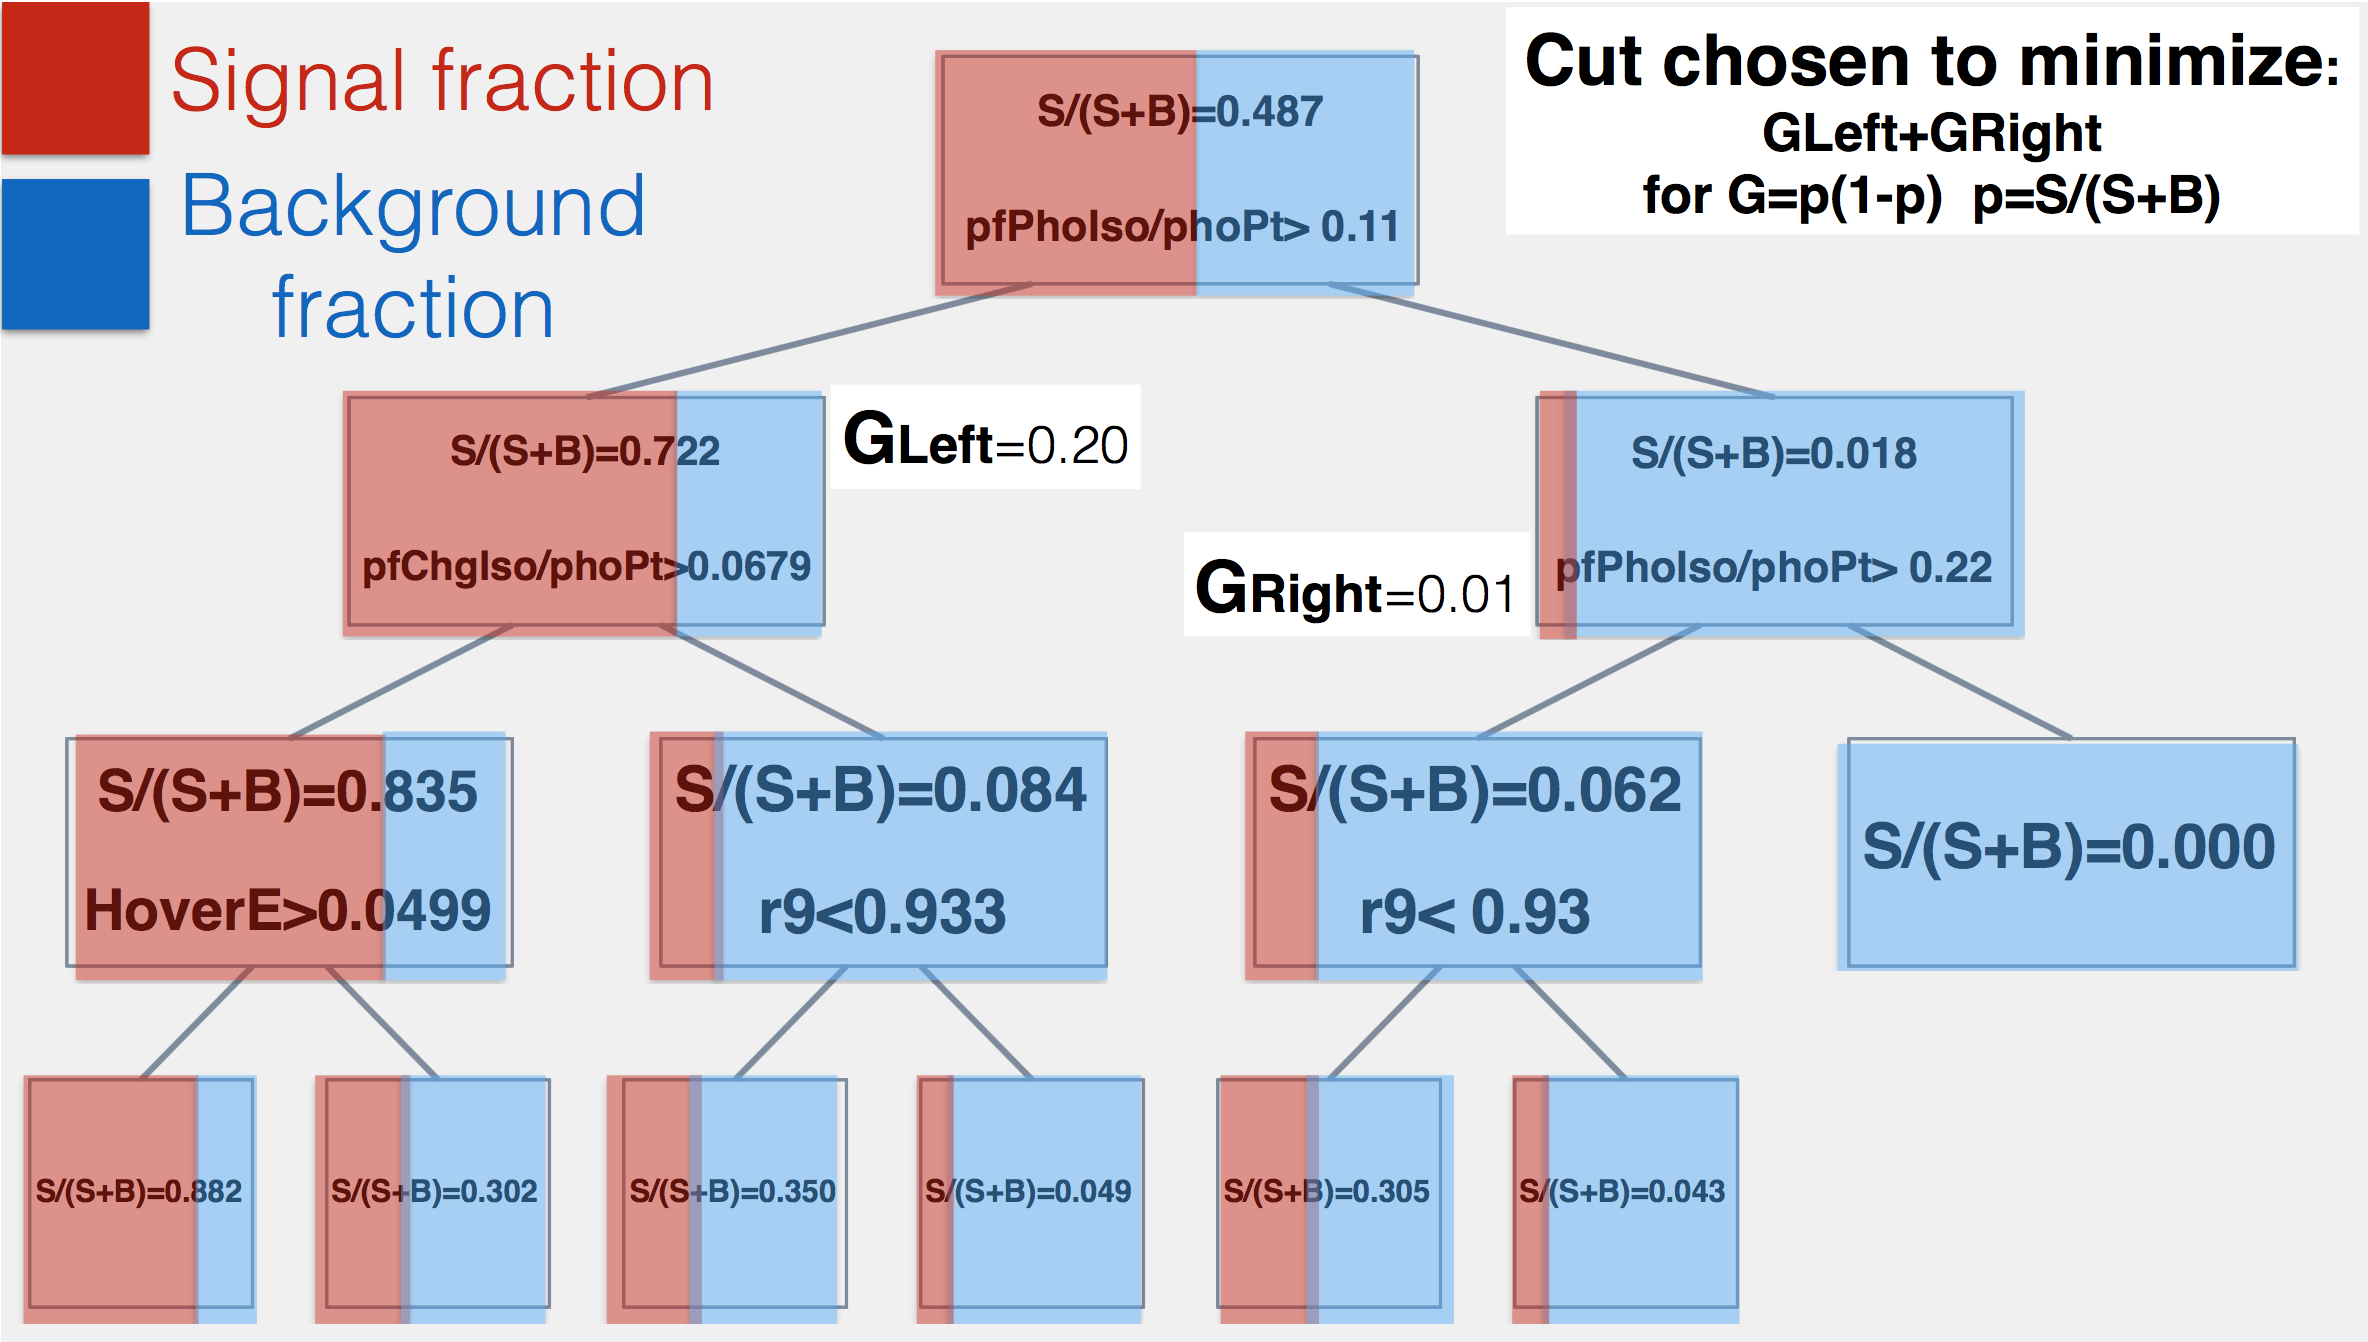
\includegraphics[width=0.95\textwidth]{\figpath/Chapter5/BDT_Classifier_Example.png}
    \caption{Example BDT classifier tree showing the cut optimization procedure to separate signal and background events. The colors within each node represent the purity $p$. The root note contains equal amounts of signal and background, but after the first layer the right-most node contains almost pure background while the left-most node contains $~$70\% signal. The base of the tree provides a node with more than 80\% signal purity.}
    \label{fig:BDT_Classifier_Example}
\end{figure}

\begin{figure}[!hbt]
    \centering
    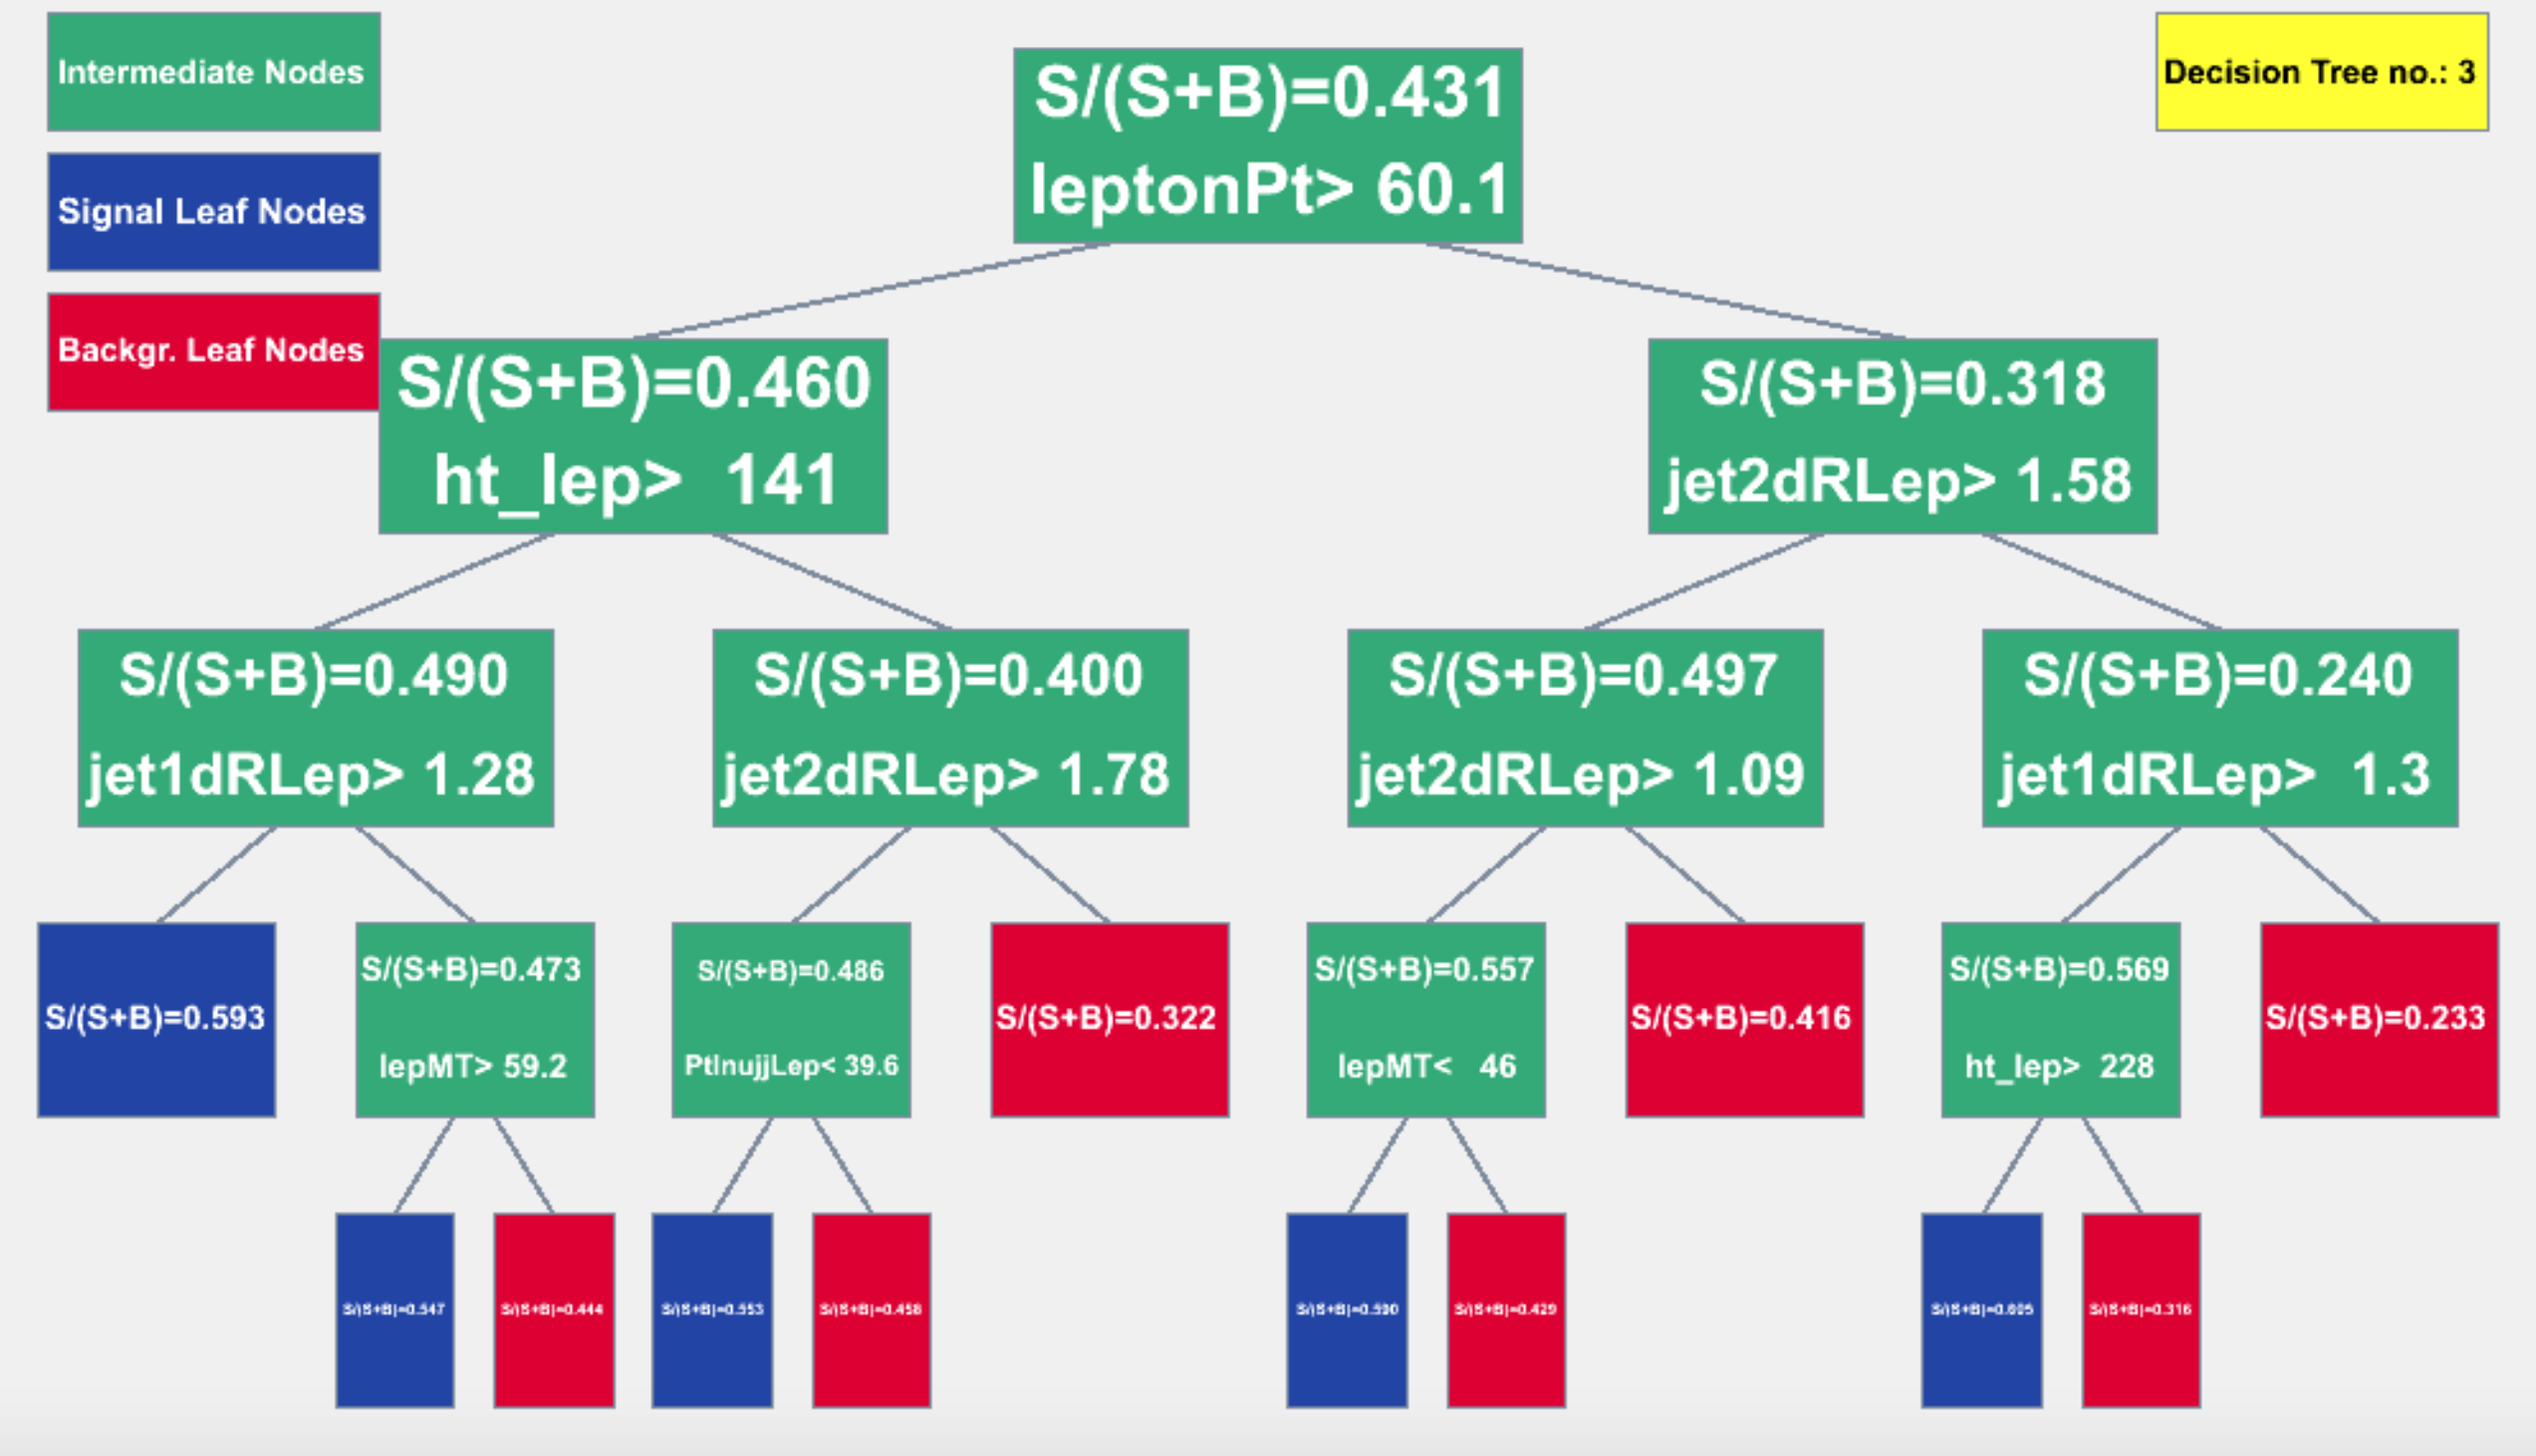
\includegraphics[width=0.95\textwidth]{\figpath/Chapter5/BDT_tree_HWWlvjj.png}
    \caption{An example decision tree used by this analysis. This tree will be combined with a forest of other trees using the boosting algorithm. The bottom nodes are defined as being more signal or background like based on the majority population left in the node.}
    \label{fig:BDT_tree_HWWlvjj}
\end{figure}

\begin{comment}
Boased on Rishi's thesis, but may only be applicable to gradient boosting

Training many independent decision trees without boosting will not prevent overtraining as each tree would have a different misclassification rate.
The boosting algorithm solves this by combining many decision trees (a ``forest'' of trees) to minimize the ensemble misclassification rate.
The weighted sum of the tree outputs is given by:
\begin{equation}\label{eq:decision_tree_weighted_sum}
  F\left(x\right)=\sum_{m=0}^{M}\beta_{m}f\left(x,a_{m}\right),
\end{equation}
where the $m$ trees are represented by base functions $f\left(x,a_{m}\right)$ and the set of values $\left(a_{m},\beta_{m}\right)$ are chosen to minimize a specially chosen loss function.
Note that $\beta_{m}$ improves the performance of the algorithm by reducing the learning rate.
The loss function choice determines the specific boosting procedure.
\end{comment}

Training many independent decision trees without boosting will not prevent overtraining as each tree would have a different misclassification rate.
The boosting algorithm solves this by combining many decision trees (a ``forest'' of trees) to minimize the ensemble misclassification rate.
This analysis makes use of the adaptive boost (AdaBoost) procedure, which weights higher in subsequent trees events which are mis-classified in the current tree~\cite{FREUND1997119}.
The event weights are initialized to 1, but change after the first tree.
Nevertheless, the weights in each tree are always normalized such that the sum of the weights remains constant.
The events in each new tree are weighted by multiplying the previous event weights by a boost weight $\alpha$ common to the tree.
$\alpha$ is defined as:
\begin{equation}
  \alpha=\frac{1-err}{err},
\end{equation}
where $err$ is the mis-classification rate of the previous tree.
%For the AdaBoost algorithm the combined weight, a modification to equation~\ref{eq:decision_tree_weighted_sum}, is given by:
The weighted sum of the tree outputs is given by:
\begin{equation}
  y_{\text{Boost}}\left(\textbf{x}\right)=\frac{1}{M}\sum_{m=0}^{M}\ln\left(\alpha_{m}\right)h_{m}\left(\textbf{x}\right),
\end{equation}
where there are $m$ trees, $\textbf{x}$ are the input variables, and $h\left(\textbf{x}\right)\in\{-1,1\}$ is the single event classifier indicating if the event is signal, $h\left(\textbf{x}\right)=1$, or background, $h\left(\textbf{x}\right)=-1$.
The resulting discriminant on the event at the end of the training, $y_{\text{Boost}}\left(\textbf{x}\right)$, is a number in the range $[1,-1]$, where 1 is most signal-like and -1 is most background-like.

The AdaBoost procedure is ideal for use with shallow trees with two or three levels each, leaving a relatively large population of events in each of the final nodes.
These are also known as weak classifiers and provide little discrimination power on their own.
The benefit to using these is that they are much less prone to overtraining, but they can be grouped together, through the boosting procedure, to provide good discrimination power.
Had the trees been allowed to reach a state where a single event was left in a node, this would imply that there was a cut sequence that would lead to perfect signal versus background classification, a practical impossibility.
It is therefore important that the analyzer keep this in mind when specifying the stopping hyper-parameters.
One of the other hyper-parameters specific to the AdaBoost procedure is the boost weight exponent, where $\alpha{\rightarrow}\alpha^{\beta}$.
By changing $\beta$ one can slow down the learning rate, allowing for a larger number of boost iterations.
The list of tunable hyper-parameters is as follows:
\begin{itemize}
  \item NTrees: The number of trees in the forest.
  \item nEventsMin: The minimum number of events allowed in a node after the splitting.
  \item MaxDepth: The maximum number of levels in the tree aside from the root node.
  \item BoostType: The boosting method to use. This analysis used the adaptive boost (AdaBoost) method, but other options are available.
  \item AdaBoostBeta: The exponent of the AdaBoost weight. This analysis used $\beta=0.5$.
  \item SeparationType: While this analysis used the Gini Index there are other choices for measuring the separation of signal and background.
  \item nCuts: The number of steps available for a single variable when determining the cut value. Increasing this number leads to finer granularity, the benefit of which was not seen by this analysis. We chose to use a step size of 20.
  \item PruneMethod: It is possible to prune away some branches to increase performance. This was unnecessary for this analysis as it used a boost procedure which limited the size of the tree.
  \item NodePurityLimit: This parameter determines at which purity ($P>\text{NodePurityLimit}$) the final node is considered a signal node. This analysis used a value of 0.5.
\end{itemize}

As an additional way to check for overtraining, one can reserve a set of events to use as a testing sample to check the efficacy of the classifier response.
The amount of signal and background to split off is tunable, but this analysis used half of the events for training and the other half for testing.
When comparing the training and testing distributions the Kolomogrov-Smirnoff test\footnote{The value returned by this test is the probability that the two distributions originated from the same probability distribution.} is used to determine their compatibility.
For this analysis a separate BDT is trained for each jet category and is individually optimized based on the chosen input variables and the hyper-parameters of the training algorithm.
Section~\ref{sec:kin_var_sel} will discuss the selection of the potential kinematic variables while sections~\ref{sec:BDT_input_optimization} and ~\ref{sec:BDT_parameter_optimization} will discuss the optimization of the inputs and parameters, respectively, for the individual trainings.

\subsection{Kinematic Variable Selection}
\label{sec:kin_var_sel}

While it may be tempting to use the 4-vectors of the final state objects as inputs to the BDT, shallow networks, like the ones used here, are not very good at learning the intricacies necessary to discriminate physics processes based on simple inputs.
Conversely, networks can be subject to sever overtraining if too many high level variables are used as input.
Instead, the user must choose a select set of input distributions to use, preferably ones that already has some separation between the signal(s) and  background(s).
It is also a good idea to provide the BDT only the dominant signal and background to train on, so as to develop a classifier with the maximal amount of separation power.
Given table~\ref{tab:yields_KinMEBDT}, we used the normalized \Wjets background and \HWW signal MC as input samples.
A list of variables with possible separation powers was then created.
Each variable's separation power was quantified using the two figures of merit (FOM) listed in equation~\ref{eq:BDT_FOM1} and~\ref{eq:BDT_FOM2}, where $i$ denotes the bin number in the distribution.
\begin{align}
  FOM1 = {}& \sum_{i=1}^{nBins}\left(\text{signal}-\text{background}\right)^{2}\label{eq:BDT_FOM1}\\
  FOM2 = {}& \sum_{i=1}^{nBins}\frac{\left(\text{signal}-\text{background}\right)^{2}}{\left(\text{signal}+\text{background}\right)^{2}}\label{eq:BDT_FOM2}
\end{align}
Fig.~\ref{fig:BDT_FOM} shows several of these distributions with their associated figures of merit.

\begin{figure}[!hbt]
    \centering
    \begin{subfigure}[t]{0.48\textwidth}
        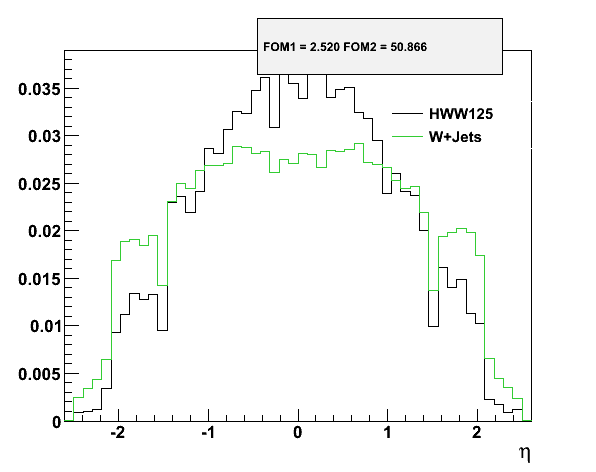
\includegraphics[width=\textwidth]{\figpath/Chapter5/BDT_InputVarOpt/lepEta.png}
        \caption{}
        \label{fig:BDT_FOM_lepEta}
    \end{subfigure}
    \begin{subfigure}[t]{0.48\textwidth}
        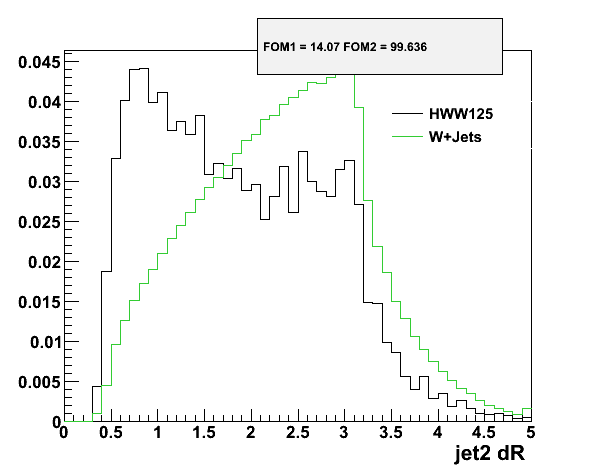
\includegraphics[width=\textwidth]{\figpath/Chapter5/BDT_InputVarOpt/jet2dRLep.png}
        \caption{}
        \label{fig:BDT_FOM_DeltaRLepJet}
    \end{subfigure}

    \begin{subfigure}[t]{0.48\textwidth}
        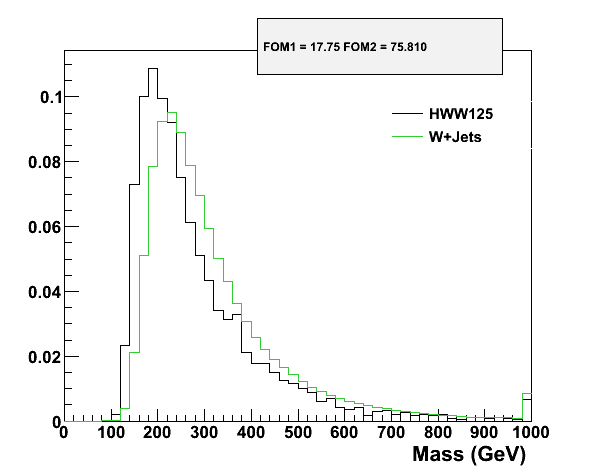
\includegraphics[width=\textwidth]{\figpath/Chapter5/BDT_InputVarOpt/MWWTop2jets.png}
        \caption{}
        \label{fig:BDT_FOM_Mlvjj}
    \end{subfigure}
    \begin{subfigure}[t]{0.48\textwidth}
        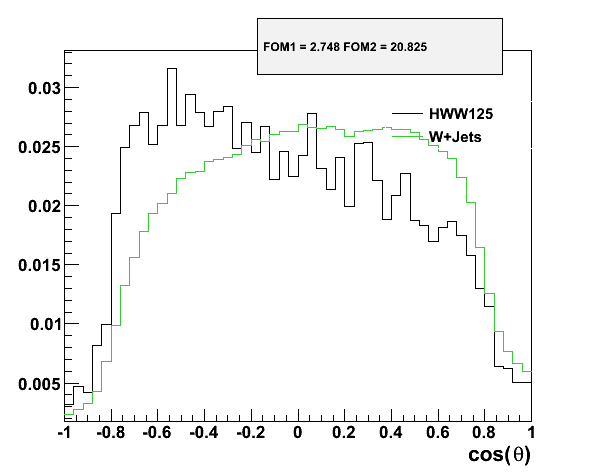
\includegraphics[width=\textwidth]{\figpath/Chapter5/BDT_InputVarOpt/CosTheta_l.png}
        \caption{}
        \label{fig:BDT_FOM_CosThetaL}
    \end{subfigure}
    \caption{Example distributions used to examine possible input variables to the BDT trainings. The \ggH (black) and \Wjets (green) samples are both unit normalized. The two FOMs calculated are shown, but since these are normalized distributions the resulting numbers would be quite small. Thus the FOM have been multiplied by $10^{5}$ for ease of reading. The four distributions are (a) lepton $\eta$, (b) $\DR\left(\Pl,\text{jet2}\right)$, (c) \Mlvjj, and (d) \costhetal.}
    \label{fig:BDT_FOM}
\end{figure}

An additional method for determining useful variables is to calculate the cumulative distribution function (CDF) for each of the variables being tested.
The CDF histograms are built bin-by-bin from the nominal distributions of each variable.
The contents of any given bin in the CDF are equal to the sum of that bin and all of the previous bins in the nominal distribution as shown in equation~\ref{eq:CDF}.
\begin{equation}\label{eq:CDF}
  C_{i}^{\text{CDF}}=\sum_{\text{bin}=0}^{i}C_{i}^{\text{nominal}}
\end{equation}
Fig.~\ref{fig:CDF_example} shows the PDF for the lepton \pt variable and the corresponding CDF.
We are looking for variables which maximize the difference between the signal and background curves.
To this end we also calculate FOM1 and FOM2 for the CDF distributions.

\begin{figure}[!hbt]
    \centering
    \begin{subfigure}[t]{0.48\textwidth}
        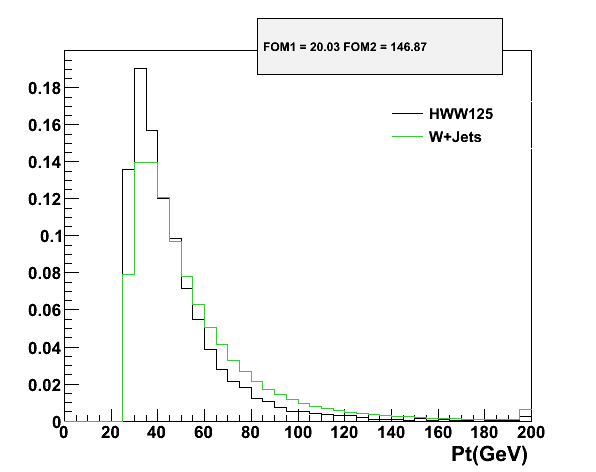
\includegraphics[width=\textwidth]{\figpath/Chapter5/BDT_InputVarOpt/lepPt.png}
        \caption{}
        \label{fig:lepPt_nominal}
    \end{subfigure}
    \begin{subfigure}[t]{0.48\textwidth}
        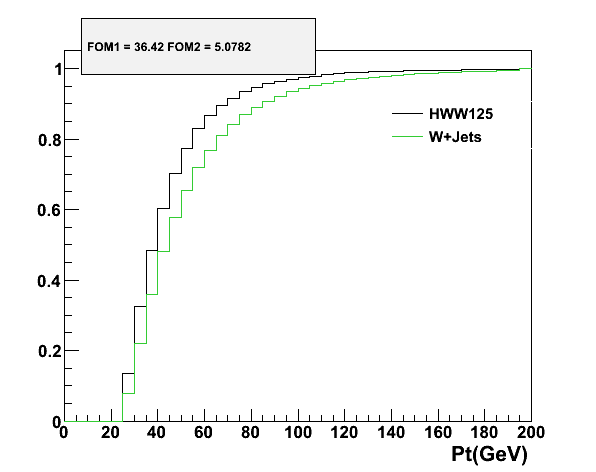
\includegraphics[width=\textwidth]{\figpath/Chapter5/BDT_InputVarOpt/lepPt_cumulative.png}
        \caption{}
        \label{fig:lepPt_CDF}
    \end{subfigure}
    \caption{(a) Nominal and (b) CDF distributions for the lepton \pt variable. The signal is shown in black and the background in green.}
    \label{fig:CDF_example}
\end{figure}

The variables were then ranked based on these four FOM values, separately for each jet bin, and only the top 20 variables in each jet bin were chosen to move on.
The final ranking was achieved by averaging the rankings of the four methods, the purpose of which was to remove any undue method bias.
Section~\ref{sec:BDT_input_optimization} will discuss the specific variables chosen for each jet bin.
However, a list of all variables considered can be found in table~\ref{tab:all_possible_BDT_kinematic_variables}.
The lepton and jet 4-vectors are denoted with \Pl and \cPj, respectively, with the jets sorted in order of descending \pt.
Some of the variable definitions are listed below:
\begin{itemize}
  \item ${{}\pt}_{x}$: The \pt of object $x$ in the event.
  \item ${{}\eta}_{x}$: The $\eta$ of object $x$ in the event.
  \item ${{}\varphi}_{x}$: The $\varphi$ of object $x$ in the event.
  \item \Mt: The transverse component of the mass of the leptonically decaying \W boson.
  \item $\Delta{R}\left(\Pl,\cPj_{\text{1}}\right)$: The distance in $R$ between the lepton and the highest \pt jet ($\Delta{R}=\sqrt{\Delta\Phi^{2}+\Delta\eta^{2}}$).
  \item $HT$: The scalar sum of the lepton \pt and the \ET of all jets in the event
  \item $\Mlvjj$: The 4-body mass defined as the mass of the vector sum of the lepton, \VETslash, and the two highest \pt jets in the event.
  \item ${{}\pt}_{\lvjj}$: The \pt of the 4-body system created by summing the 4-vectors of the lepton, \VETslash, and the two highest \pt jets in the event.
  \item $\Delta{R}\left(\Pl,\jj\right)$: The $\Delta{R}$, as defined above, between the lepton and the di-jet system formed by the two highest \pt jets in the event. 
  \item $\Delta\varphi\left(\VETslash,\cPj\right)$: The $\Delta\varphi$ between the leading jet and the \VETslash.
  \item $\Delta\varphi\left(\cPj,\cPj\right)$: The $\Delta\varphi$ between the two highest \pt jets in the event.
  \item $\Delta\varphi_{\text{min}}\left(\Pl,\cPj\right)$: The smallest $\Delta\varphi$ between the lepton and any of the jets in the event.
  \item $\Delta\eta\left(\cPj,\cPj\right)$: The $\eta$ between the two highest \pt jets in the event.
  \item $\text{CSV}_{disc.}\left(\cPj_{i}\right)$: The CSV discriminant value for jet $i$.
\end{itemize}

\begin{table}[htbp]
\centering
\begin{tabular}{cc} \hline
$\cos\left(\Delta\Phi_{\WH}\right)$ & $\cos\left(\Delta\Phi_{\WW}\right)$ \\
$\cos\left(\theta_{\cPj}\right)$ & $\cos\left(\theta_{\Pl}\right)$ \\
$\cos\left(\theta_{\WH}\right)$ & $\Delta\eta\left(\cPj,\cPj\right)$ \\
$\Delta\varphi\left(\cPj,\cPj\right)$ & $\Delta\varphi\left(\VETslash,\cPj\right)$ \\
$\Delta\varphi\left(\VETslash,\Pl\right)$ & $\Delta{R}\left(\Pl,\jj\right)$ \\
$\eta\left(\cPj,\cPj\right)$ & $HT$ \\
$\text{CSV}_{disc.}\left(\cPj_{\text{1}}\right)$ & $\text{CSV}_{disc.}\left(\cPj_{\text{2}}\right)$ \\
$\Delta{R}\left(\Pl,\cPj_{\text{1}}\right)$ & $\Delta{R}\left(\Pl,\cPj_{\text{2}}\right)$ \\
$\Delta{R}\left(\Pl,\cPj_{\text{3}}\right)$ & $\Delta{R}\left(\Pl,\cPj_{\text{4}}\right)$ \\
$\eta_{\cPj_{\text{1}}}$ & $\eta_{\cPj_{\text{2}}}$ \\
$\varphi_{\cPj_{\text{1}}}$ & $\varphi_{\cPj_{\text{2}}}$ \\
$\pt\left(\cPj_{\text{1}}\right)$ & $\pt\left(\cPj_{\text{2}}\right)$ \\
$\text{Charge}_{\Pl}$ & $\eta_{\Pl}$ \\
${{}\text{Charge}}_{\Pl}\times{{}\eta}_{\Pl}$ & ${{}\pt}_{\Pl}$ \\
$\ETslash$ & $\varphi_{\ETslash}$ \\
$\Delta\varphi_{\text{min}}\left(\Pl,\cPj\right)$ & $\Delta\varphi_{\text{min}}\left(\VETslash,\cPj\right)$ \\
$\Mjj$ & $\Mlvjj$ \\
$\Mt$ & $\text{nBTag}_{\text{CSV}_{\text{m}}}$ \\
n\textsubscript{\cPj} & n\textsubscript{\cPj\textsubscript{low}} \\
n\textsubscript{PV} & ${{}\pt}_{\lvjj}$ \\
$\sum{{}\ET}_{\cPj}$ & ${{}\pt}_{\jj}$ \\\hline
\end{tabular}
\caption{A list of all of the kinematic variables considered for inclusion in the BDT training. The variables are listed in no particular order and thus placement within the table is unimportant.}
\label{tab:all_possible_BDT_kinematic_variables}
\end{table}

In additions to the definitions listed above, the are a whole host of angular variables which in part specify the kinematics of the Higgs and \W boson decays.
When defining these variables, much of which was done in~\cite{Dobrescu2010}, it will help to refer to the diagram in fig.~\ref{fig:XWWDecayAngles}.
To start with, a kinematic fit is used to calculate the longitudinal momentum of the neutrino, $p_{z}$, and to also constrain the invariant mass of the leptonic \W, \Mlv.
Because the angle definitions are agnostic as to the type of particle decaying, the initiating particle will be referred to as particle X.
The angles are as follows:
\begin{itemize}
  \item $\theta^{*}$ is the polar angle between the collision axis $z$ and the X decay axis $z'$ as defined in the rest frame of particle X.
  \item $\Phi_{1}$ is the azimuthal angle between the $zz'$ plane and the decay plane of the hadronic \W.
  \item $\Phi$ is the angle between the decay planes of the \WW system in the rest frame of particle X.
  \item $\theta_{1}$ is the angle between the $z'$ axis the highest \pt jet, defined from 0 to $\pi$.
  \item $\theta_{2}$ is the angle between the $z'$ axis and the lepton.
\end{itemize}
Rather than using the bare angles, we have chosen to use the cosine of the angles and have thus named them as:
\begin{itemize}
  \item $\Phi{\rightarrow}\cos\left(\Delta\Phi_{\WW}\right)$
  \item $\Phi_{1}{\rightarrow}\cos\left(\Delta\Phi_{\WH}\right)$
  \item $\theta_{1}{\rightarrow}\cos\left(\theta_{\cPj}\right)$
  \item $\theta_{2}{\rightarrow}\cos\left(\theta_{\Pl}\right)$
  \item $\theta^{*}{\rightarrow}\cos\left(\theta_{\WH}\right)$
\end{itemize}

\begin{figure}[!hbt]
    \centering
    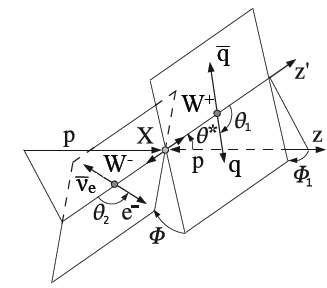
\includegraphics[width=0.95\textwidth]{\figpath/Chapter5/WDecayAngles.png}
    \caption{Planes and angular variables in the \HWWlvqq decay process~\cite{PhysRevD.81.075022}.}
    \label{fig:XWWDecayAngles}
\end{figure}

\subsection{BDT Input Optimization}
\label{sec:BDT_input_optimization}

Remember that only the \Wjets sample is being used to represent the background while a combination of the three \HWW samples is being used to represent the signal.
When training a BDT the absolute normalization of the signal samples is not what is important.
Instead, they must be normalized to their expected fractions relative to each other.
Thus, the two other samples are normalized to the $\cPg\cPg\HWW$ sample as shown in table~\ref{tab:BDT_sample_scale_factors}.
After setting up the samples the BDTs in each jet bin had to be optimized.
The procedure in section~\ref{sec:kin_var_sel} was used to select the individual variables with the most discrimination power.
This section will describe how that list of input variables was optimized for the BDT trainings in each jet bin.

\begin{table}[htbp]
\centering
\begin{tabular}{lccc} \hline
\textbf{Process} & \textbf{2 Jets} & \textbf{3 Jets} & \textbf{$\geqslant$4Jets} \\\hline
\ggH; $\MH=\text{125}\gev$, \HWWlvjj       & 1.0   & 1.0   & 1.0   \\
\qqH; $\MH=\text{125}\gev$, \HWWlvjj       & 0.195 & 0.248 & 0.239 \\
\WH, \ZH, \ttH; $\MH=\text{125}\gev$, \HWW & 0.256 & 0.416 & 0.608 \\\hline
\end{tabular}
\caption{The scale factors used to normalize the input signal samples for the BDT trainings.}
\label{tab:BDT_sample_scale_factors}
\end{table}

To begin with, a BDT was trained using the best 20 variables specified in the previous section.
After that, the BDT was checked for redundant variables by looking at the input variable correlation plots and for overtraining by using the Kolmogorov-Smirnov values between the training and test samples.
If the Kolmogorov-Smirnov score was too low, this setup was rejected as it would indicate that the training and test samples didn't come from same underlying PDF, which they must.
The variables used to train the BDT were also ranked by TMVA in order of their importance, which is measured by how much a given variable was used to discriminate signal from background.
On the next iteration the two lowest performing variables were removed and the BDT was retrained.
This process continued until only three input variables remained.
Fig.~\ref{fig:KinBDT_Example_Output} contains an example response curve examining overtraining as well as the correlation plots for signal and background.
Based on the minimal correlation shown, none of the 11 variables are redundant in this training.

\begin{figure}[!hbt]
    \centering
    \begin{subfigure}[t]{0.48\textwidth}
        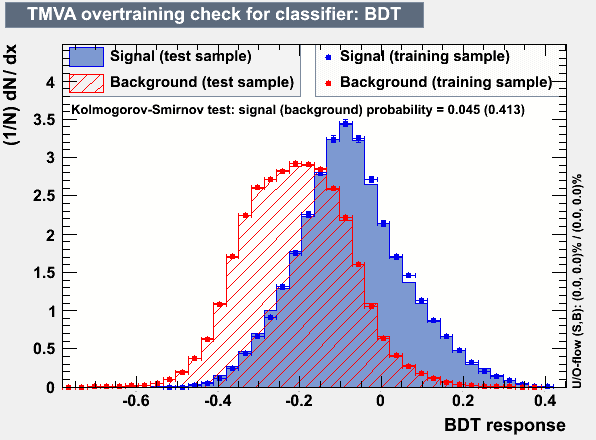
\includegraphics[width=\textwidth]{\figpath/Chapter5/BDT_Control_Plots/overtrain_2j0B_11Max4_Original.png}
        \caption{}
        \label{fig:KinBDT_Overtrain_Example}
    \end{subfigure}

    \begin{subfigure}[t]{0.48\textwidth}
        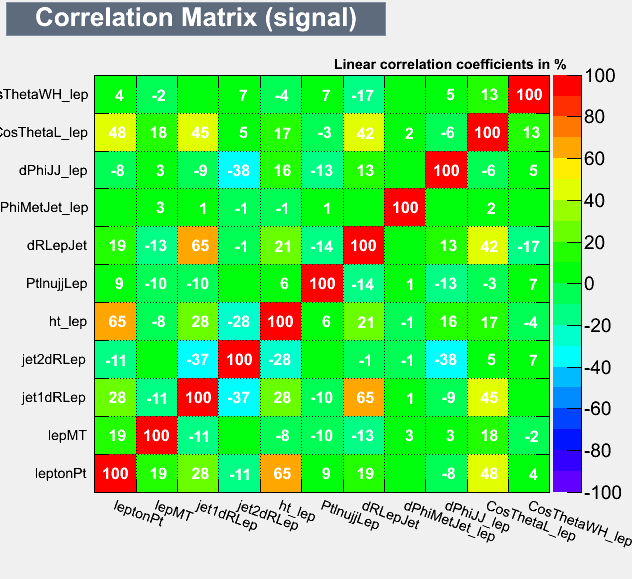
\includegraphics[width=\textwidth]{\figpath/Chapter5/BDT_Control_Plots/CorrelationMatrixS_2j0B.png}
        \caption{}
        \label{fig:KinBDT_CorrelationMatrixS_Example}
    \end{subfigure}
    \begin{subfigure}[t]{0.48\textwidth}
        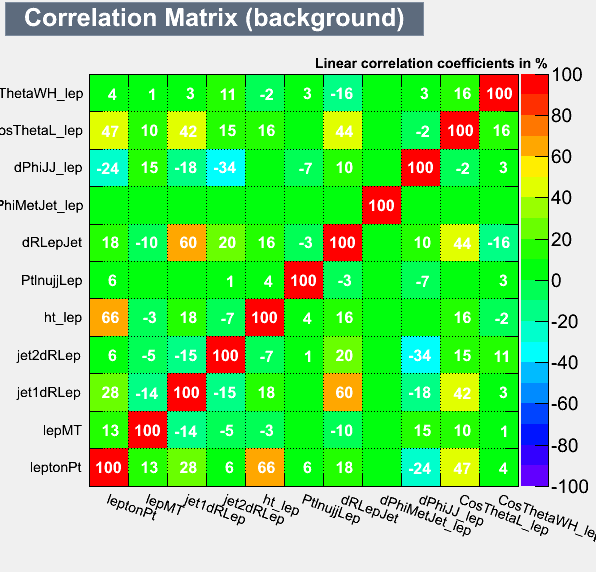
\includegraphics[width=\textwidth]{\figpath/Chapter5/BDT_Control_Plots/CorrelationMatrixB_2j0B.png}
        \caption{}
        \label{fig:KinBDT_CorrelationMatrixB_Example}
    \end{subfigure}
    \caption{Example validation plots after the BDT training. (a) The response distributions for signal and background for both the training (markers) and test samples (filled histograms). The Kolmogorov-Smirnov value is used to decide how much overtraining has occurred. The correlation matrices of the input variables for the (b) signal and (c) background samples.}
    \label{fig:KinBDT_Example_Output}
\end{figure}

To quantitatively compare the various trainings we made use of their respective receiver operating characteristic (ROC) curves, an example of which is shown in fig.~\ref{fig:KinBDT_ROC_Output_Example}.
These curves measure the performance of a binary classification system by testing the signal efficiency and background rejection assuming a cut is placed on the classifier output.
There are several ways of using the ROC curve to test the overall performance of any one BDT training.
While a common method is to use the area under the ROC curve (greater area means better performance), we chose to use a different measure.
Since the point (1,1) represents perfect signal acceptance and background rejection, that is the ideal point.
A training with a ROC curve whose distance to that point is minimized will perform better than any other training.
Thus we chose to use this distance as our FOM between the various trainings.

\begin{figure}[!hbt]
    \centering
    \begin{subfigure}[t]{0.48\textwidth}
        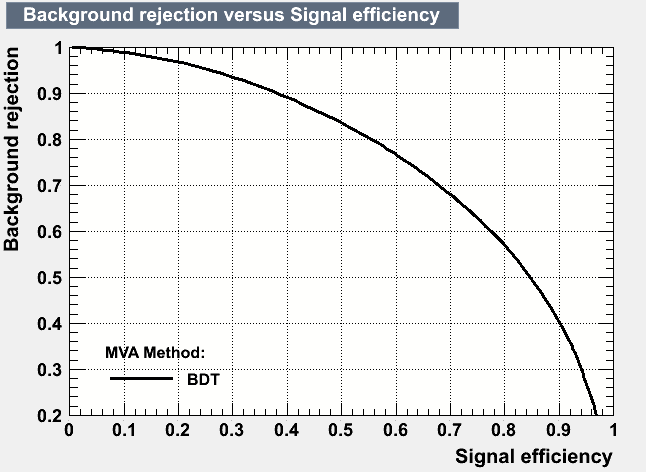
\includegraphics[width=\textwidth]{\figpath/Chapter5/BDT_Control_Plots/rejBvsS.png}
        \caption{}
        \label{fig:KinBDT_ROC_Output_Example}
    \end{subfigure}
    \begin{subfigure}[t]{0.48\textwidth}
        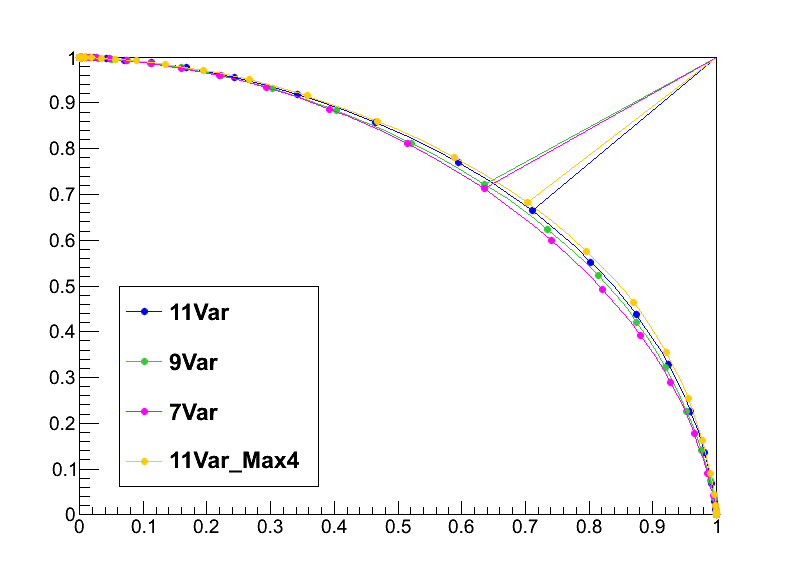
\includegraphics[width=\textwidth]{\figpath/Chapter5/BDT_Control_Plots/ROC_Overlay_Compare.png}
        \caption{}
        \label{fig:KinBDT_ROC_nVarComparison}
    \end{subfigure}
    \caption{Example ROC curved produced after the BDT training. (a) A standard ROC curve produced by TMVA. (b) ROC curves from multiple trainings with their associated distances of closest approach calculated. The training using 11 input variables showed the most discrimination power.}
    \label{fig:KinBDT_ROC_Examples}
\end{figure}

The ROC curves from the multiple trainings were compared as seen in fig.~\ref{fig:KinBDT_ROC_nVarComparison}.
Although reducing the number of variables can help to prevent overtraining, there comes a point when this process begins to negatively impact the performance of the BDT.
By comparing the ROC curves we were able to identify the trainings with the best performance.
The variables used in these trainings are identified in table~\ref{tab:BDT_variables_optimized}.
The validation plots for the input variables can be found in appendix~\ref{appendix:BDT_Inputs}.

\begin{table}[htbp]
\centering
\begin{tabular}{lccc} \hline
\textbf{Variable} & \textbf{2 Jets} & \textbf{3 Jets} & \textbf{$\geqslant$4Jets} \\\hline
${{}\pt}_{\Pl}$                                   & $\bigstar$   & $\checkmark$ &              \\
${{}\text{Charge}}_{\Pl}\times{{}\eta}_{\Pl}$     &              & $\checkmark$ & $\checkmark$ \\
$\Mt$                                             & $\checkmark$ &              &              \\
${{}\pt}_{\lvjj}$                                 & $\checkmark$ &              &              \\
$\Mlvjj$                                          &              & $\checkmark$ & $\checkmark$ \\
HT                                                & $\checkmark$ & $\bigstar$   & $\bigstar$   \\
$\Delta{R}\left(\Pl,\cPj_{\text{1}}\right)$       & $\checkmark$ &              &              \\
$\Delta{R}\left(\Pl,\cPj_{\text{2}}\right)$       & $\checkmark$ & $\checkmark$ & $\checkmark$ \\
$\Delta{R}\left(\Pl,\cPj_{\text{3}}\right)$       &              & $\checkmark$ & $\checkmark$ \\
$\Delta{R}\left(\Pl,\jj\right)$                   & $\checkmark$ & $\checkmark$ &              \\
$\Delta\varphi_{\text{min}}\left(\Pl,\cPj\right)$ &              & $\checkmark$ &              \\
$\Delta\eta\left(\cPj,\cPj\right)$                &              & $\checkmark$ &              \\
$\Delta\varphi\left(\VETslash,\cPj\right)$        & $\checkmark$ & $\checkmark$ & $\checkmark$ \\
$\Delta\varphi\left(\VETslash,\Pl\right)$         &              &              & $\checkmark$ \\
$\Delta\varphi\left(\cPj,\cPj\right)$             & $\checkmark$ &              &              \\
$\cos\left(\theta_{\Pl}\right)$                   & $\checkmark$ & $\checkmark$ &              \\
$\cos\left(\theta_{\WH}\right)$                   & $\checkmark$ & $\checkmark$ &              \\
$\cos\left(\theta_{\cPj}\right)$                  &              & $\checkmark$ &              \\\hline
\end{tabular}
\caption{A list of the input variables chosen for each BDT training. The variables are optimized separately in each jet bin. The check marks denote the chosen variables for each jet bin while the stars denote the the best performing variable.}
\label{tab:BDT_variables_optimized}
\end{table}

\subsection{BDT Parameter Optimization}
\label{sec:BDT_parameter_optimization}

Besides the number of input variables, there are several hyper-parameters for the BDT trainings which must also be optimized to extract the maximum amount of performance and reduce the amount of overtraining.
These hyper-parameters include the maximum number of trees to using in the training (nTrees), the value of $\beta$ used in the boosting procedure (adaBoostBeta), the maximum depth allowed for each tree (MaxDepth), the minimum number of events allowed to remain in a node after splitting (nEventsMin), and the fraction of signal versus background events used during training.
The trainings optimized for the input variables were used as a baseline for these next trainings.
Each hyper-parameter was varied individually to see its effect on the performance of the BDT.

\begin{figure}[!hbt]
    \centering
    \begin{subfigure}[t]{0.48\textwidth}
        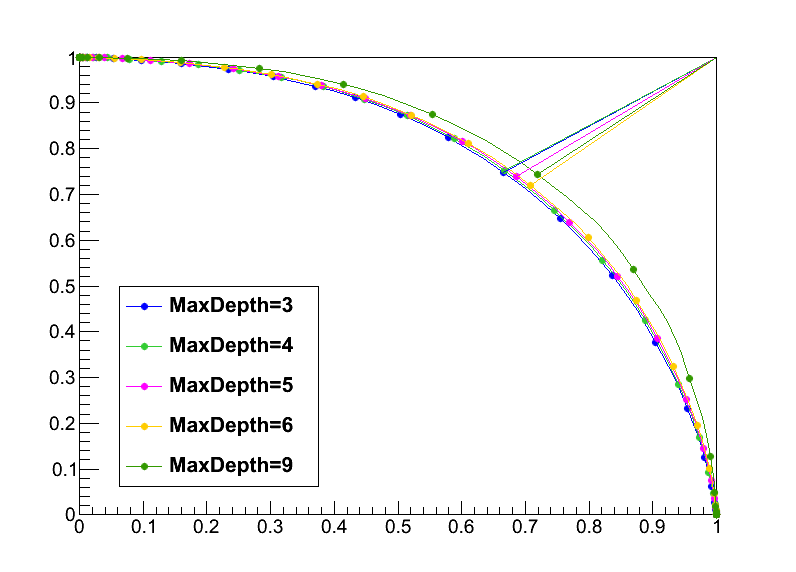
\includegraphics[width=\textwidth]{\figpath/Chapter5/BDT_Control_Plots/MaxDepthROC.png}
        \caption{}
        \label{fig:KinBDT_ROC_MaxDepth}
    \end{subfigure}

    \begin{subfigure}[t]{0.48\textwidth}
        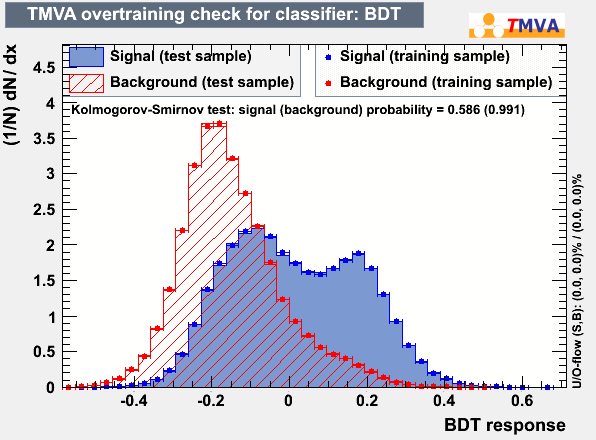
\includegraphics[width=\textwidth]{\figpath/Chapter5/BDT_Control_Plots/overtrain_BDT_Max3.png}
        \caption{}
        \label{fig:KinBDT_Ovetrain_MaxDepth3}
    \end{subfigure}
    \begin{subfigure}[t]{0.48\textwidth}
        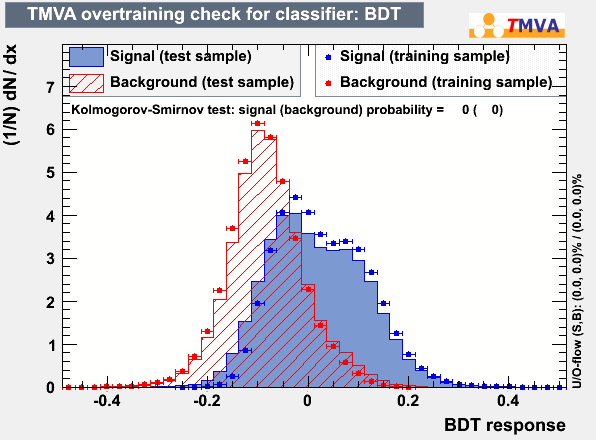
\includegraphics[width=\textwidth]{\figpath/Chapter5/BDT_Control_Plots/overtrain_BDT_Max9.png}
        \caption{}
        \label{fig:KinBDT_Ovetrain_MaxDepth9}
    \end{subfigure}
    \caption{(a) The ROC curve used to test the performance of five different values of the MaxDepth parameter. The overtraining plots showing the BDT response for MaxDepth values of (b) 3 and (c) 9. The Kolmogorov-Smirnov scores for a MaxDepth of 3 are far superior to those for a MaxDepth of 9.}
    \label{fig:KinBDT_MaxDepth_Example}
\end{figure}

\begin{figure}[!hbt]
    \centering
    \begin{subfigure}[t]{0.48\textwidth}
        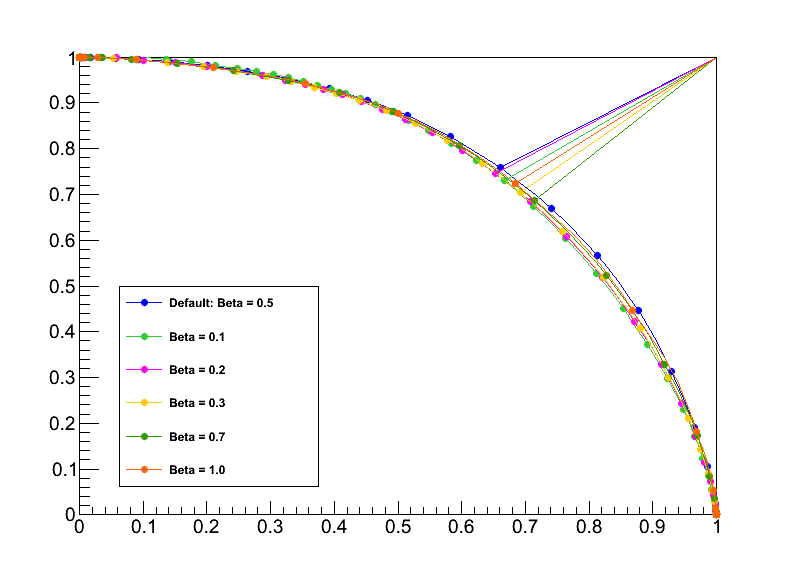
\includegraphics[width=\textwidth]{\figpath/Chapter5/BDT_Control_Plots/ROC_Overlay_Compare_AdaBoostBeta.png}
        \caption{}
        \label{fig:KinBDT_ROC_AdaBoostBeta}
    \end{subfigure}
    \begin{subfigure}[t]{0.48\textwidth}
        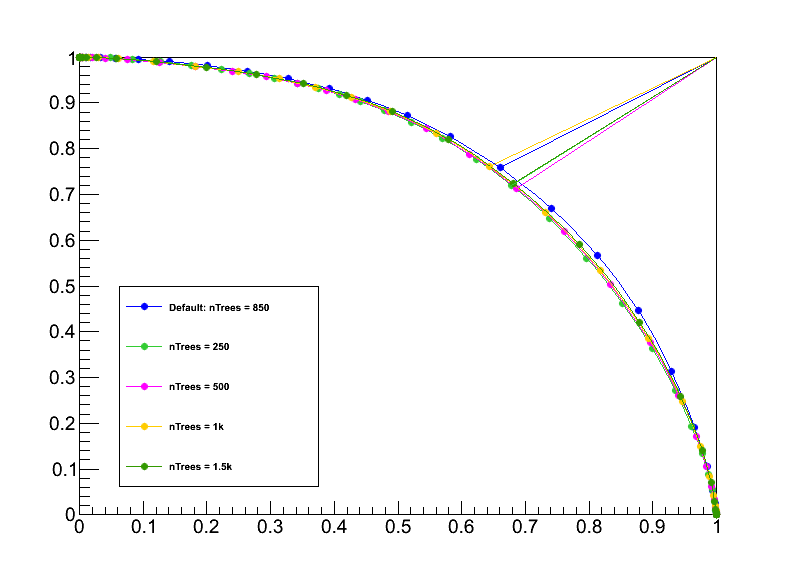
\includegraphics[width=\textwidth]{\figpath/Chapter5/BDT_Control_Plots/ROC_Overlay_Compare_nTrees.png}
        \caption{}
        \label{fig:KinBDT_ROC_nTrees}
    \end{subfigure}
    \caption{The ROC curves used to test the performance of different values of (a) the adaptive boost factor $\beta$ and (b) the number of trees used in the trainings. The best performing value is represented by the dark blue curve.}
    \label{fig:KinBDT_AdaBoostBeta_nTrees_Example}
\end{figure}

The ROC curves and overtraining plots for the tests on the MaxDepth parameter are shown in fig.~\ref{fig:KinBDT_MaxDepth_Example}.
Although increasing the depth of the trees results in improved performance, it also significantly increases the overtraining.
Thus we chose the largest MaxDepth value that didn't result in overtraining.
The ROC comparisons for the parameters adaBoostBeta and nTrees is are shown in fig.~\ref{fig:KinBDT_AdaBoostBeta_nTrees_Example}.
In these cases, the default values turned out to be the best performing.
The final hyper-parameter values used for our trainings can be found in table~\ref{tab:BDT_hyper-parameter_values}.
We also found that using the maximum possible amount of signal and background events was best, meaning we fed the trainings all the events that we had.
The events were then split evenly between the test and training samples.
The resultant BDT classifier distributions are shown in appendix~\ref{appendix:BDT_Outputs}.

\begin{table}[htbp]
\centering
\begin{tabular}{lccc} \hline
\textbf{Hyper-Parameter} & \textbf{2 Jets} & \textbf{3 Jets} & \textbf{$\geqslant$4Jets} \\\hline
MaxDepth    & 4   & 3   & 3 \\
nTrees      & 850 & 850 & 850 \\
adaBootBeta & 0.5 & 0.5 & 0.5 \\
nEventsMin  & 100 & 100 & 100 \\\hline
\end{tabular}
\caption{}
\label{tab:BDT_hyper-parameter_values}
\end{table}

\section{Matrix Element Analysis}

Table~\ref{tab:yields_KinMEBDT} clearly shows that the total signal, in every channel, is at least an order of magnitude smaller than even the statistical uncertainty of the background.
A simple cut and count experiment will not lead to any significant results.
The previous \HWWlnujj analyses have performed a fit to sensitive distributions like the 4-body mass, the mass of the system made out of the two jets, lepton, and \ETslash, which is sensitive to the Higgs mass peak.
However, this approach only includes a small amount of available information, leaving out additional sensitive kinematic distributions.
It is also felt that a BDT analysis using only kinematic variable would be sub-optimal because shallow classifiers are not robust against non-linear correlations and are only as good as the input variables chosen.
While the BDT classifiers described in the last section show a good amount of signal to background discrimination, there is another method which can also be used to separate signal from background.
Instead, this analysis uses a matrix element method (MEM), which starts from the differential cross section calculation from quantum field theory to classify how likely and event is to come from a given process~\cite{Canelli2003,Dong2008}.

\subsection{Differential Cross Section}

The probability $P\left(x;\alpha\right)=P_{evt}$ of a signal is proportional to the differential production cross section, where $\alpha$ is the parameter we wish to measure, like the mass of the Higgs boson, and x is a set of physical variables.
This is true if the detector resolution is sufficiently small and the beam energies are well known, as it is in the case of CMS.
For the scattering of two particles the differential cross section can be written as~\cite{Olive:2016xmw}:
\begin{equation}\label{eq:differential_production_cross_section}
d\sigma=\frac{\left(2\pi\right)^{4}|\mathcal{M}|^{2}}{4\sqrt{\left(q_{1}\cdot{q_{2}}\right)^{2}-m_{q_{1}}^{2}m_{q_{2}}^{2}}}d\Phi_{n}\left(q_{1}+q_{2};p_{1},...,p_{n}\right)
\end{equation}
where $|\mathcal{M}|$ is the Lorentz invariant matrix element (ME)~\cite{Griffiths2008}; $q_{1}$, $q_{2}$ and $m_{1}$, $m_{2}$ are the 4-momenta and masses of the incident particles; $p_{i}$ are the 4-momenta of the $n$ final state particles; and $d\Phi_{n}$ is the n-body phase space.
The phase space term is written as:
\begin{equation}
d\Phi_{n}\left(q_{1}+q_{2};p_{1},...,p_{n}\right)=\delta^{4}\left(q_{1}+q_{2}-\sum_{i=1}^{n}p_{i}\right)\prod_{i=1}^{n}\frac{d^{3}p_{i}}{\left(2\pi\right)^{3}2E_{i}}
\end{equation}

If CMS could measure all of the final state particles with 100\% accuracy, no detector effects or uncertainties, and all of the information about the initial state particles was known - including the energy, momentum, and particle type - we could analytically solve this equation and normalize it to the total cross section to define an event probability $P_{evt}\sim\frac{d\sigma}{\sigma}$.
Using the differential cross sections for each of the processes being tested we could create a perfect discriminant for each event.
Unfortunately, this is not the case and there are several unknowns which must be accounted for:
\begin{enumerate}
  \item Some particles involved in the ME are either not measured at all or not fully measured. The initial state partons are held within protons, making their exact energies unknown. The neutrino in the final state is not fully measured by CMS. We use the \ETslash as a proxy for the neutrino, but we can't measure the $p_{z}$ component of its momentum vector.
  \item The partons in the final state are only measured after showering and hadronizing to form jets. While every effort is taken to measure the jet energies with great accuracy, this is no substitute for the parton level energies.
  \item The energy resolution of the CMS sub-detectors cannot be ignored, especially for jets.
  \item For practical reasons the ME cannot be exactly calculated. The more precise a probability one wants to calculate, the more diagrams one must include in the ME calculation. This increases the computational complexity of the problem significantly. That is why this analysis used mainly tree-level diagrams, with some sub-leading diagrams for our biggest background, \Wjets.
\end{enumerate}
Despite our best efforts, each of these effects leads to some loss in sensitivity.

\subsection{Parton Distribution Functions and Phase Space}

if final state fully known (momenta and energies), then can calculate the initial state momenta and energies from conservation of energy and momentum, assuming the transverse momentum of the initial state particles is zero (a fairly good assumption).
Without knowing the full final state, a set of PDFs will determine the likelihood of a given initial state configuration.
The PDF scale varies with the process dependent momentum transfer $\text{Q}^{2}$.
For \Wjets, for example, $\text{Q}^{2}=\MW^{2}+\left(\sum_{\text{jets}}\pt\right)^{2}$ while for Drell-Yan scattering $\text{Q}^{2}=\hat{s}=|q_{1}+q_{2}|^{2}$, where $q_{1}$ and $q_{2}$ are 4-vectors of the initial state quarks.
Because $\text{Q}^{2}$ comes from perturbative calculations and cannot be measured, its value is not well defined~\cite{Dong2008}.

Taking this into account, the differential cross section calculation becomes:
\begin{equation}
d\sigma=\frac{\left(2\pi\right)^{4}|\mathcal{M}|^{2}}{4\sqrt{\left(q_{1}\cdot{q_{2}}\right)^{2}-m_{q_{1}}^{2}m_{q_{2}}^{2}}}f\left(x_{1}\right)f\left(x_{2}\right)d\Phi_{n}\left(q_{1}+q_{2};p_{1},...,p_{n}\right),
\end{equation}
where $f\left(x_{i}\right)$ are the PDFs for the incoming protons and $x_{i}=E_{q_{i}}/E_{beam}$ is the fraction of the proton momentum carried by the incident parton $i$.
%Even for diagrams with unique quarks it's still not clear which parton came from which proton.
%In this case both probabilities are computed and added together.

The differential cross section can be further simplified by using $\sqrt{\left(q_{1}{\cdot}q_{2}\right)^{2}-m_{q_{1}}^{2}m_{q_{2}}^{2}}\simeq2E_{q_{1}}E_{q_{2}}$.
In other words by considering the input partons to be massless and ignoring any small transverse momentum they may have we arrive at:
\begin{equation}
d\sigma=2\pi^{4}|\mathcal{M}|^{2}\frac{f\left(x_{1}\right)}{|E_{q_{1}}|}\frac{f\left(x_{2}\right)}{|E_{q_{2}}|}d\Phi_{n}\left(q_{1}+q_{2};p_{1},...,p_{n}\right).
\end{equation}

\subsection{Transfer Functions}

While leptons in CMS can be measured with a high degree of accuracy, the lepton resolution is relatively small, the jet energies are not the same as the energies of their initiating partons.
Even worse are the neutrinos which pass all the way through the CMS detector without being measured.
The solution is to use a transfer function, which maps between the energies and momenta of the final state partons to those of the measured objects.
Adding a transfer function $W$ into the differential cross section calculation we find:
\begin{equation}
d\sigma=2\pi^{4}|\mathcal{M}|^{2}\frac{f\left(x_{1}\right)}{|E_{q_{1}}|}\frac{f\left(x_{2}\right)}{|E_{q_{2}}|}W_{l}^{3}\left(p_{l},p_{l_{\text{meas}}}\right)W_{\nu}^{3}\left(p_{\nu},p_{\nu_{\text{meas}}}\right)\prod_{i=1}^{n_{\text{jets}}}W_{i}^{3}\left(p_{i},p_{i_{\text{meas}}}\right)d\Phi_{n}\left(q_{1}+q_{2};p_{1},...,p_{n}\right)
\end{equation}
Here $W^{3}$ refers to the three transfer functions necessary to map the energy, polar angle, and azimuthal angle of the parton to the observed quantity.

Luckily we can start making some simplifications right off the bat.
The lepton quantities and jet angles are assumed to be measured well enough that the transfer function approaches a Dirac delta function.
Even if this isn't exactly true it would only reduce the sensitivity of the analysis and would not affect the final result.
Thus those terms will disappear from the equation.
Unfortunately, the same assumptions cannot be made about the jet energies.
The jet energy transfer functions are modeled as a ten parameter double Gaussian fit to the difference in parton and jet energies from a MC sample.
The underlying distribution of energies can be seen in fig.~\ref{fig:JetEnergyVsUDSGenJetEnergy}.
While matching parton energies and jet energies might sound a lot like the L5Flavor corrections in CMS, the JEC only correct the jet energies back to the most probable value.
By using a transfer function we can integrate across all possible jet energies to extract more information.
Although the transfer functions will vary across $\eta$ we had limited statistics available in out MC sample used to derive these and thus were forced to use a single bin of \absetalt{2.4}.
Three different sets of TF were derived for \cPqb quark jets, light quark jets, and gluon jets as seen in fig.~\ref{fig:Ep-Ej}.
All three types of jets will have different kinematics and thus will produce different transfer functions.
%Can't remember what sample was used to produce these

\begin{figure}[!hbt]
    \centering
    \begin{subfigure}[t]{0.48\textwidth}
        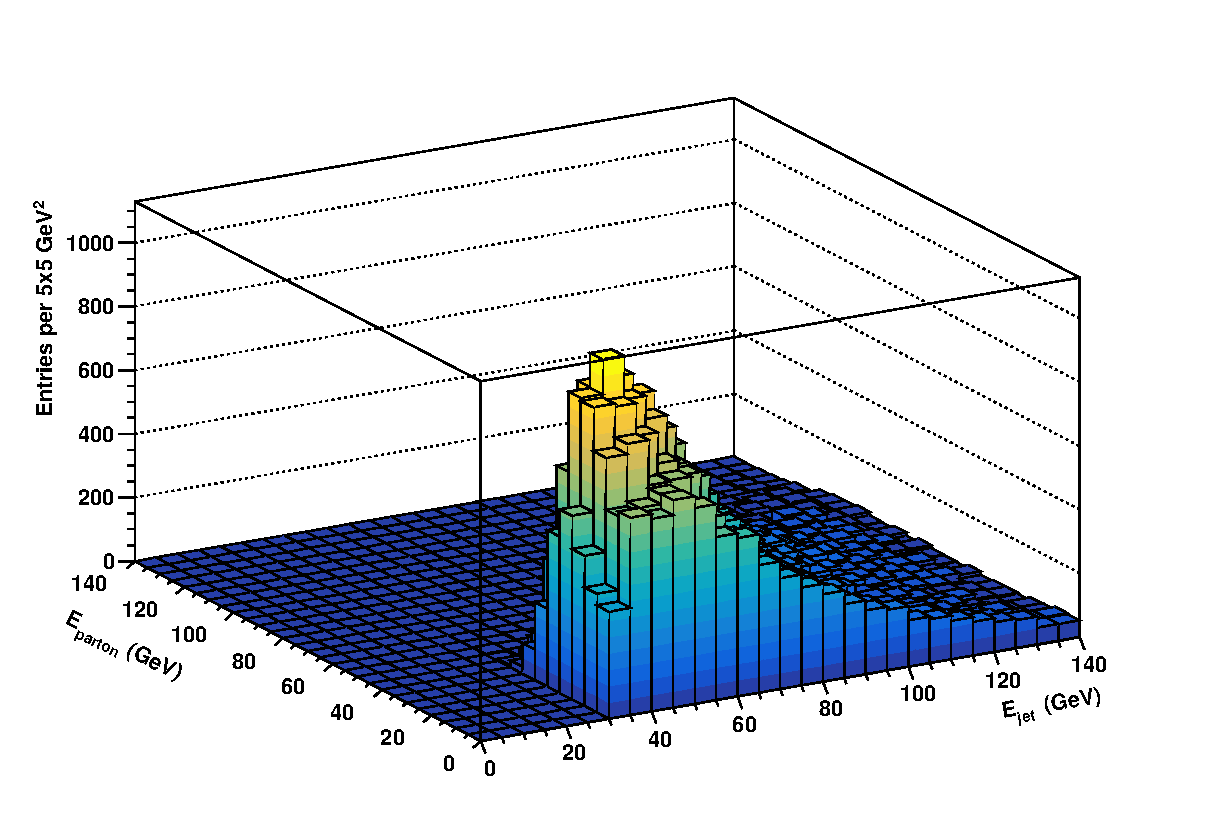
\includegraphics[width=\textwidth]{\figpath/Chapter5/JetEnergyVsUDSGenJetEnergy_0.eps}
        \caption{}
        \label{fig:JetEnergyVsUDSGenJetEnergy}
    \end{subfigure}
    \begin{subfigure}[t]{0.48\textwidth}
        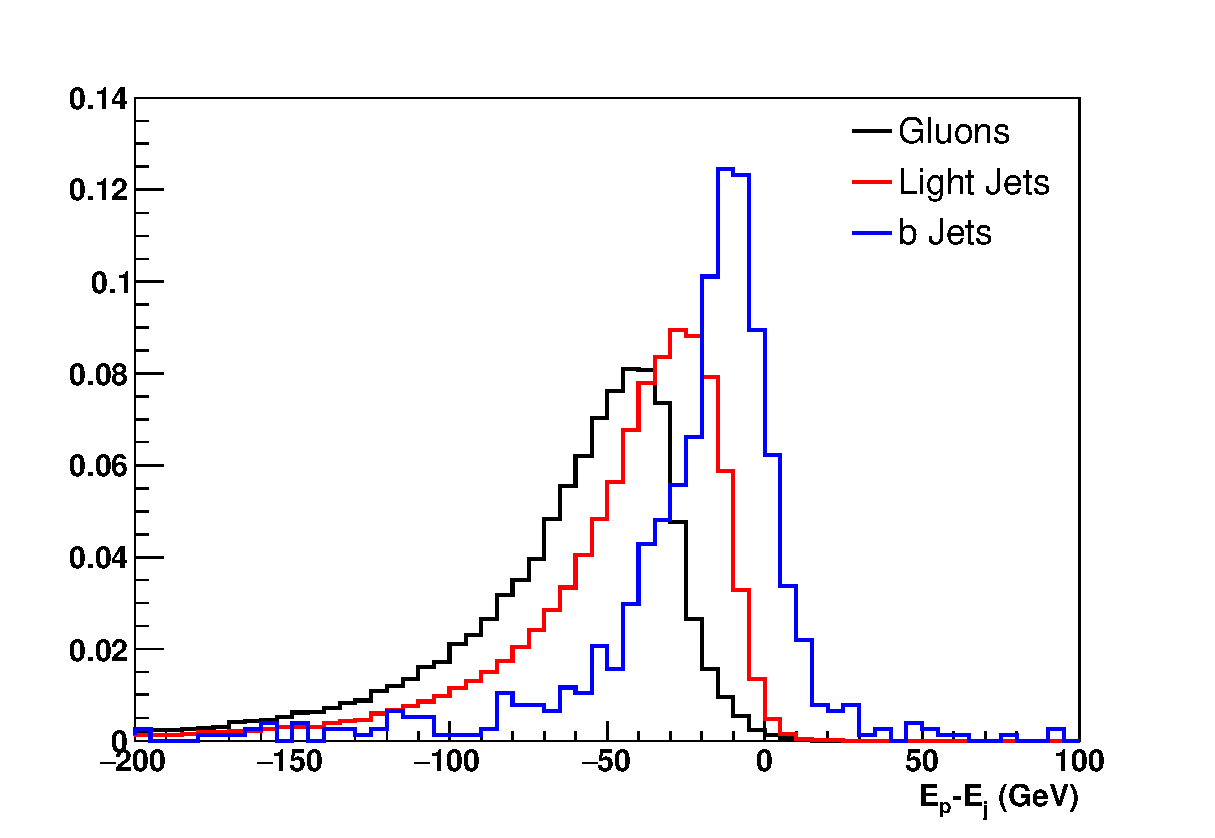
\includegraphics[width=\textwidth]{\figpath/Chapter5/Ep-Ej.eps}
        \caption{}
        \label{fig:Ep-Ej}
    \end{subfigure}
    \caption{(a) The distribution of parton energy versus jet energy in Monte Carlo events for light flavored jets. (b) Distributions of the difference in parton energy and jet energy for different kinds of jets. This proves that a separate transfer function is necessary for each flavor of jet.}
    \label{fig:transfer_functions}
\end{figure}


As stated before, the neutrino momentum is not measured; nor can the $z$ component of the neutrino momentum cannot be calculated.
This stems from the fact that the longitudinal momentum of the initial state partons is not know, only the momentum of the protons.
We don't know how the momentum is split between the various partons that make up the proton.
During the computation of the differential cross section we integrate over the unknown quantities, which includes the neutrino's longitudinal momentum.
The momentum is allowed to vary from 0\gev to 4\tev, the beam energy, which is motivated by the conservation of energy and momentum.
At this point, assuming a choice for neutrino $p_{z}$ and jet energies, the $x$ and $y$ components of the neutrino momentum as well as the $z$ component of the momenta for the initial partons can be derived from conservation of energy and momentum.

After accounting for all the simplifications, the PDFs, and the transfer functions the differential cross section becomes:
\begin{equation}
  d\sigma=\int dp_{z_{\nu}}2\pi^{4}|\mathcal{M}|^{2}\frac{f\left(x_{1}\right)}{|E_{q_{1}}|}\frac{f\left(x_{2}\right)}{|E_{q_{2}}|}\prod_{i=1}^{n_{\text{jets}}}\frac{dE_{i}W\left(E_{i},E_{i_{\text{meas}}}\right)}{E_{i}}\frac{\delta^{4}\left(q_{1}+q_{2}-p_{l}-p_{\nu}-\sum_{i=1}^{n_{\text{jets}}}p_{i}\right)}{E_{l}E_{\nu}}
\end{equation}
Ass you can see all of the parton level quantities have been replaces by their measured counterparts, which allows us to perform the calculations with the measurements taken by CMS.
This equation can then be normalized to the total cross section to form an event probability:
\begin{equation}
P(x;\alpha)=\frac{1}{\sigma}\int2\pi^{4}|\mathcal{M}|^{2}\frac{f\left(x_{1}\right)}{|E_{q_{1}}|}\frac{f\left(x_{2}\right)}{|E_{q_{2}}|}W\left(y,x\right)d\Phi_{4}dE_{q_{1}}dE_{q_{2}}
\end{equation}
where $f\left(x_{i}\right)$ are the PDFs, $x_{i}=E_{q_{i}}/E_{beam}$ is the fraction of the proton momentum carried by the incident parton $i$, and $W\left(y,x\right)$ is the transfer function mapping measured jet energies $x$ to the parton energies $y$.
For simplicity the equation has been returned to a more compact form.
At this point we can use numerical integration to calculate the the probability densities of interest.

\subsection{Matrix Elements}

As I alluded to before, no analytic form for a scattering process matrix element to all orders exists.
On top of an already computationally difficult problem, the loop corrections in higher-order calculations become too costly, which is why we chose to use mostly leading order diagrams (except for \Wjets).
The matrix elements were generated by \textsc{Mad}\textsc{Graph} in FORTRAN and then converted by C++ to speed up computation.\footnote{Only the leading diagrams were converted. The C++ code was then run alongside the FORTRAN code to compare the outputs.}
\textsc{Mad}\textsc{Graph} makes use of a library called HELAS~\cite{Murayama:1992gi} to do the leading-order matrix element calculations.
Each matrix elements can have contributions from multiple subprocesses (i.e. $\Pp\Pp\rightarrow\WW\rightarrow\lvjj$ includes diagrams from $\cPqu\cPaqu\rightarrow\Pep\PGne\cPaqu\cPqd$, $\cPqu\cPaqu\rightarrow\Pem\PAGne\cPqu\cPaqd$, $\cPqd\cPaqd\rightarrow\Pem\PAGne\cPqu\cPaqd$, etc.).
Additionally, each subprocess can be generated from a number of diagrams as seen in fig.~\ref{fig:MadGraph5_example_subdiagrams} for the $\cPg\cPqd\rightarrow\Pem\PAGne\cPqu\cPg$ process.

\begin{figure}[!hbt]
    \centering
    \begin{subfigure}[t]{0.9\textwidth}
        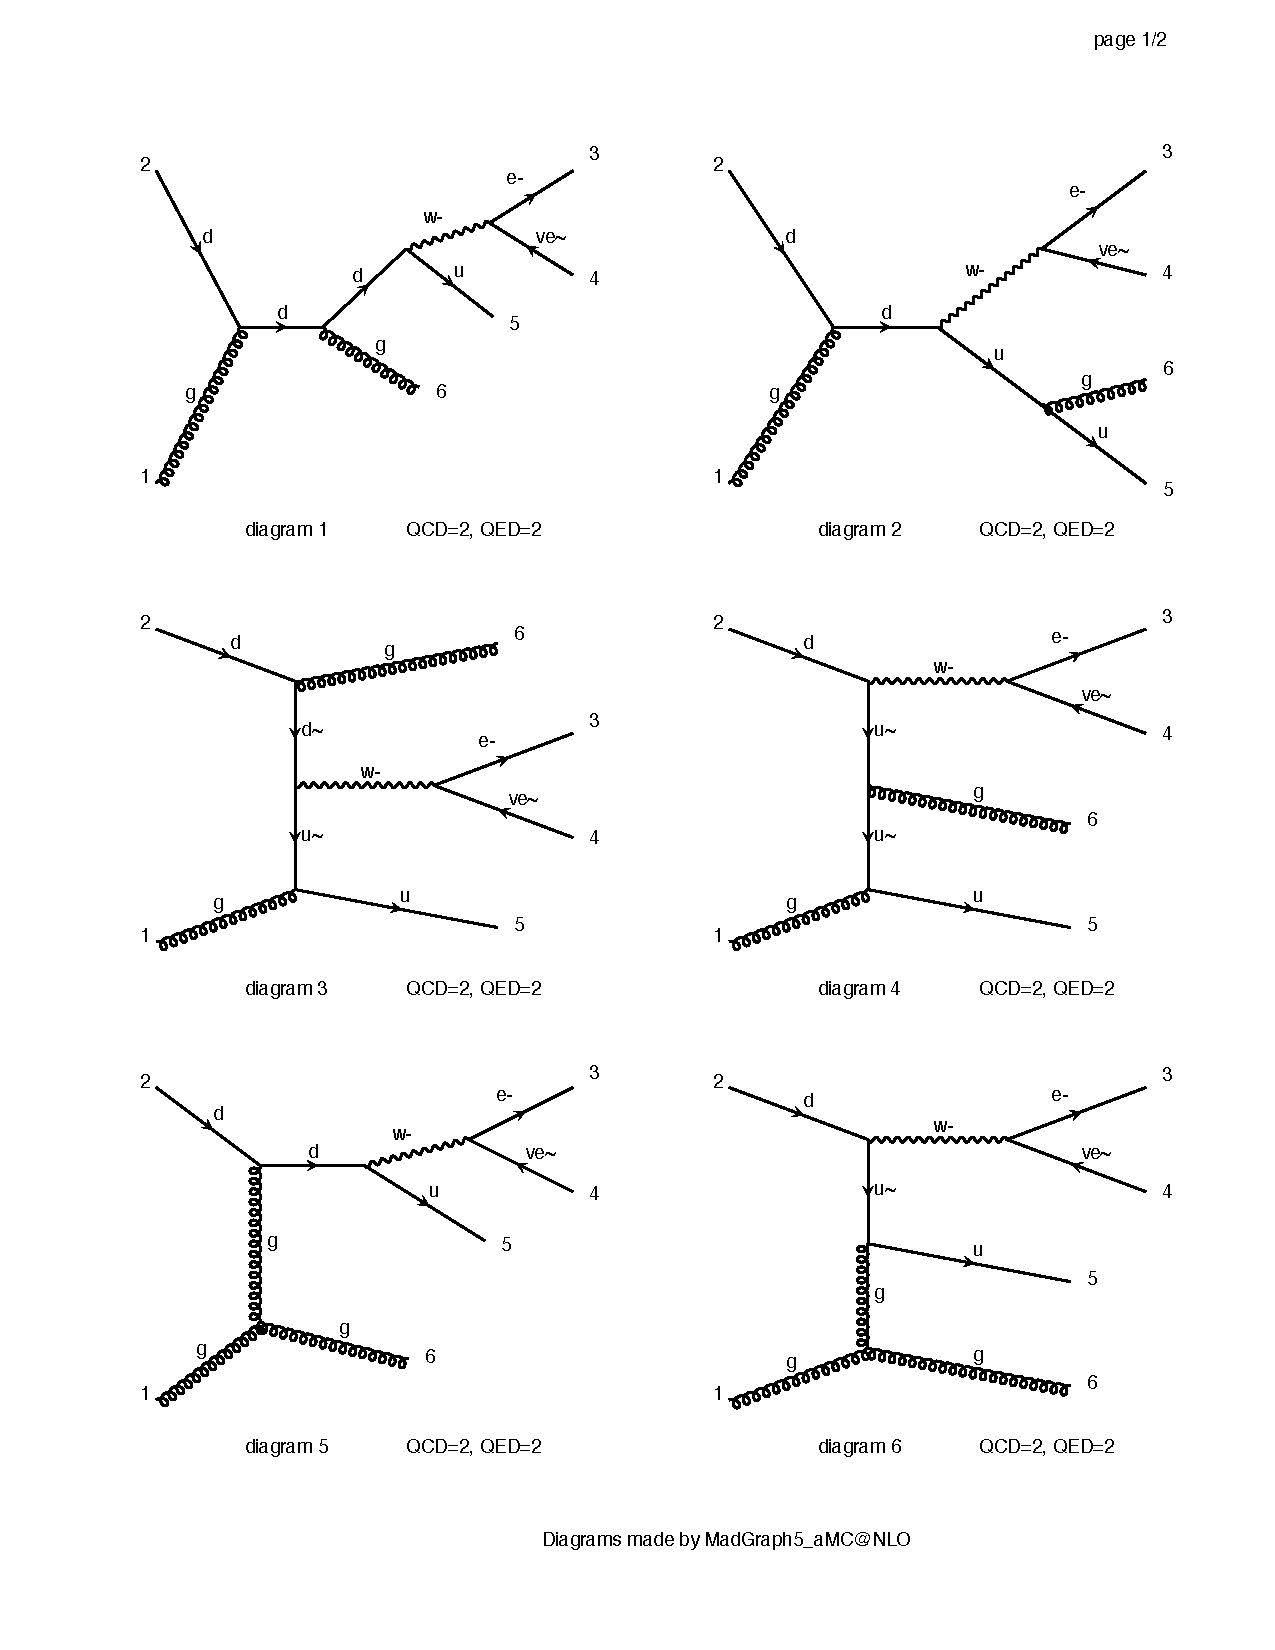
\includegraphics[width=\textwidth,page=1,trim={0 3cm 0 2cm},clip]{\figpath/Chapter5/MadGraph/g_d_-_e-_ve_u_g_matrix.pdf}
    \end{subfigure}

    \begin{subfigure}[t]{0.9\textwidth}
        \includegraphics[width=\textwidth,page=2,trim={0 7.25in 0 2cm},clip]{\figpath/Chapter5/MadGraph/g_d_-_e-_ve_u_g_matrix.pdf}
    \end{subfigure}
    \caption{Feynman diagrams from the $\cPg\cPqd\rightarrow\Pem\PAGne\cPqu\cPg$ process.}
    \label{fig:MadGraph5_example_subdiagrams}
\end{figure}

Matrix elements were calculated for all of the major signals and background in this analysis.
There were 15 matrix elements which were eventually used: \WW, \WZ, $\WZ\cPqb\cPqb$, $\W\cmsSymbolFace{L}\cPg$, $\W\cmsSymbolFace{L}\cPg$ (second order), $\W\cPg\cPg$, $\W\cmsSymbolFace{L}\cmsSymbolFace{L}$, $\W\cmsSymbolFace{L}\cPqb$, $\W\cPqb\cPqb$, ZLight, Single Top \cPqt-channel, Single Top \cPqs-channel, QCD, \ggH (\joinsym{\MH}{=}{125\gev}), and \WH (\joinsym{\MH}{=}{125\gev}).
While some matrix element diagrams may be left out, the purpose of calculating the probabilities is to discriminate a signal event from a background event.
The loss of a diagram will simply reduce the sensitivity of the classifier, not change the answer.
The some of the Feynman diagrams used for calculating the matrix elements can be found in figs.~\ref{fig:MadGraph5_example_signal} and~\ref{fig:MadGraph5_example_Wjj}.

\begin{figure}[!hbt]
    \centering
    \begin{subfigure}[t]{0.48\textwidth}
        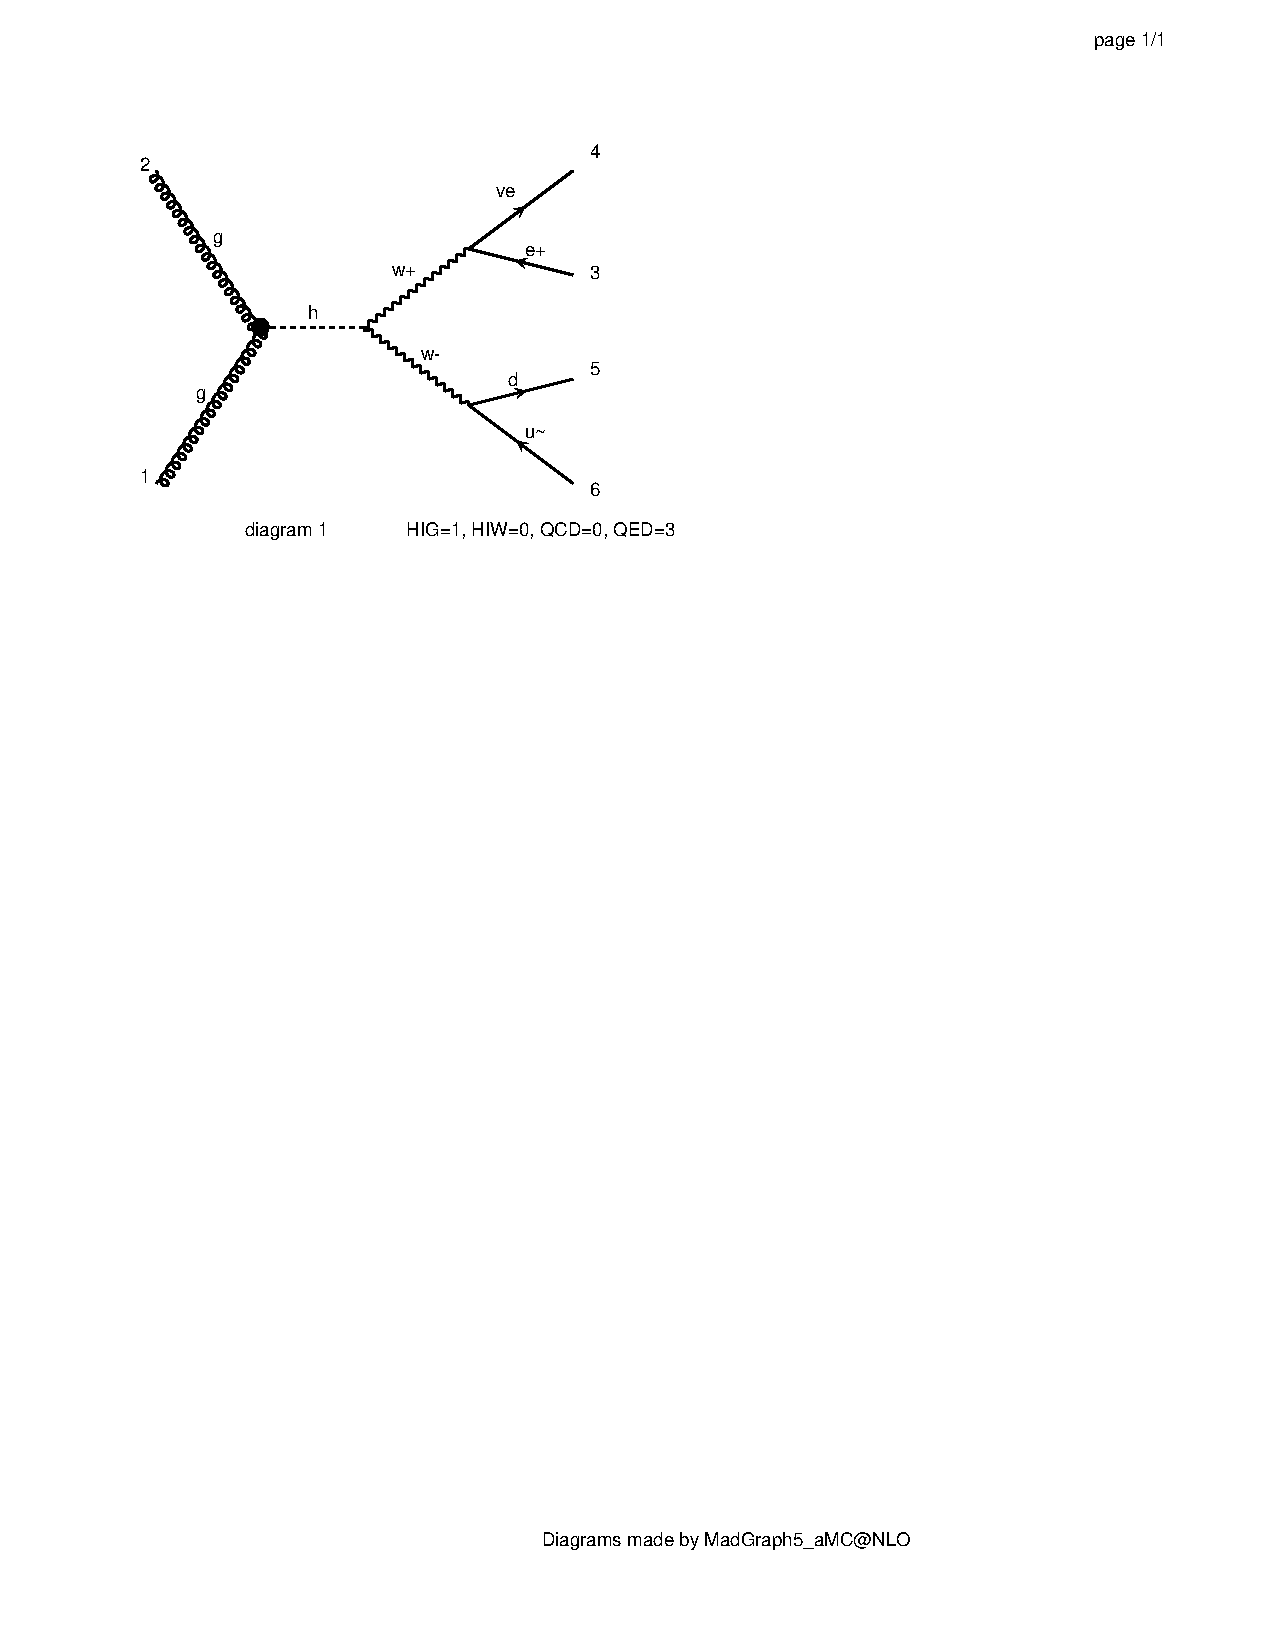
\includegraphics[width=\textwidth,trim={0.5in 7.25in 4in 2cm},clip]{\figpath/Chapter5/MadGraph/matrix_ggH_WW_lvjj.pdf}
    \end{subfigure}
    \begin{subfigure}[t]{0.48\textwidth}
        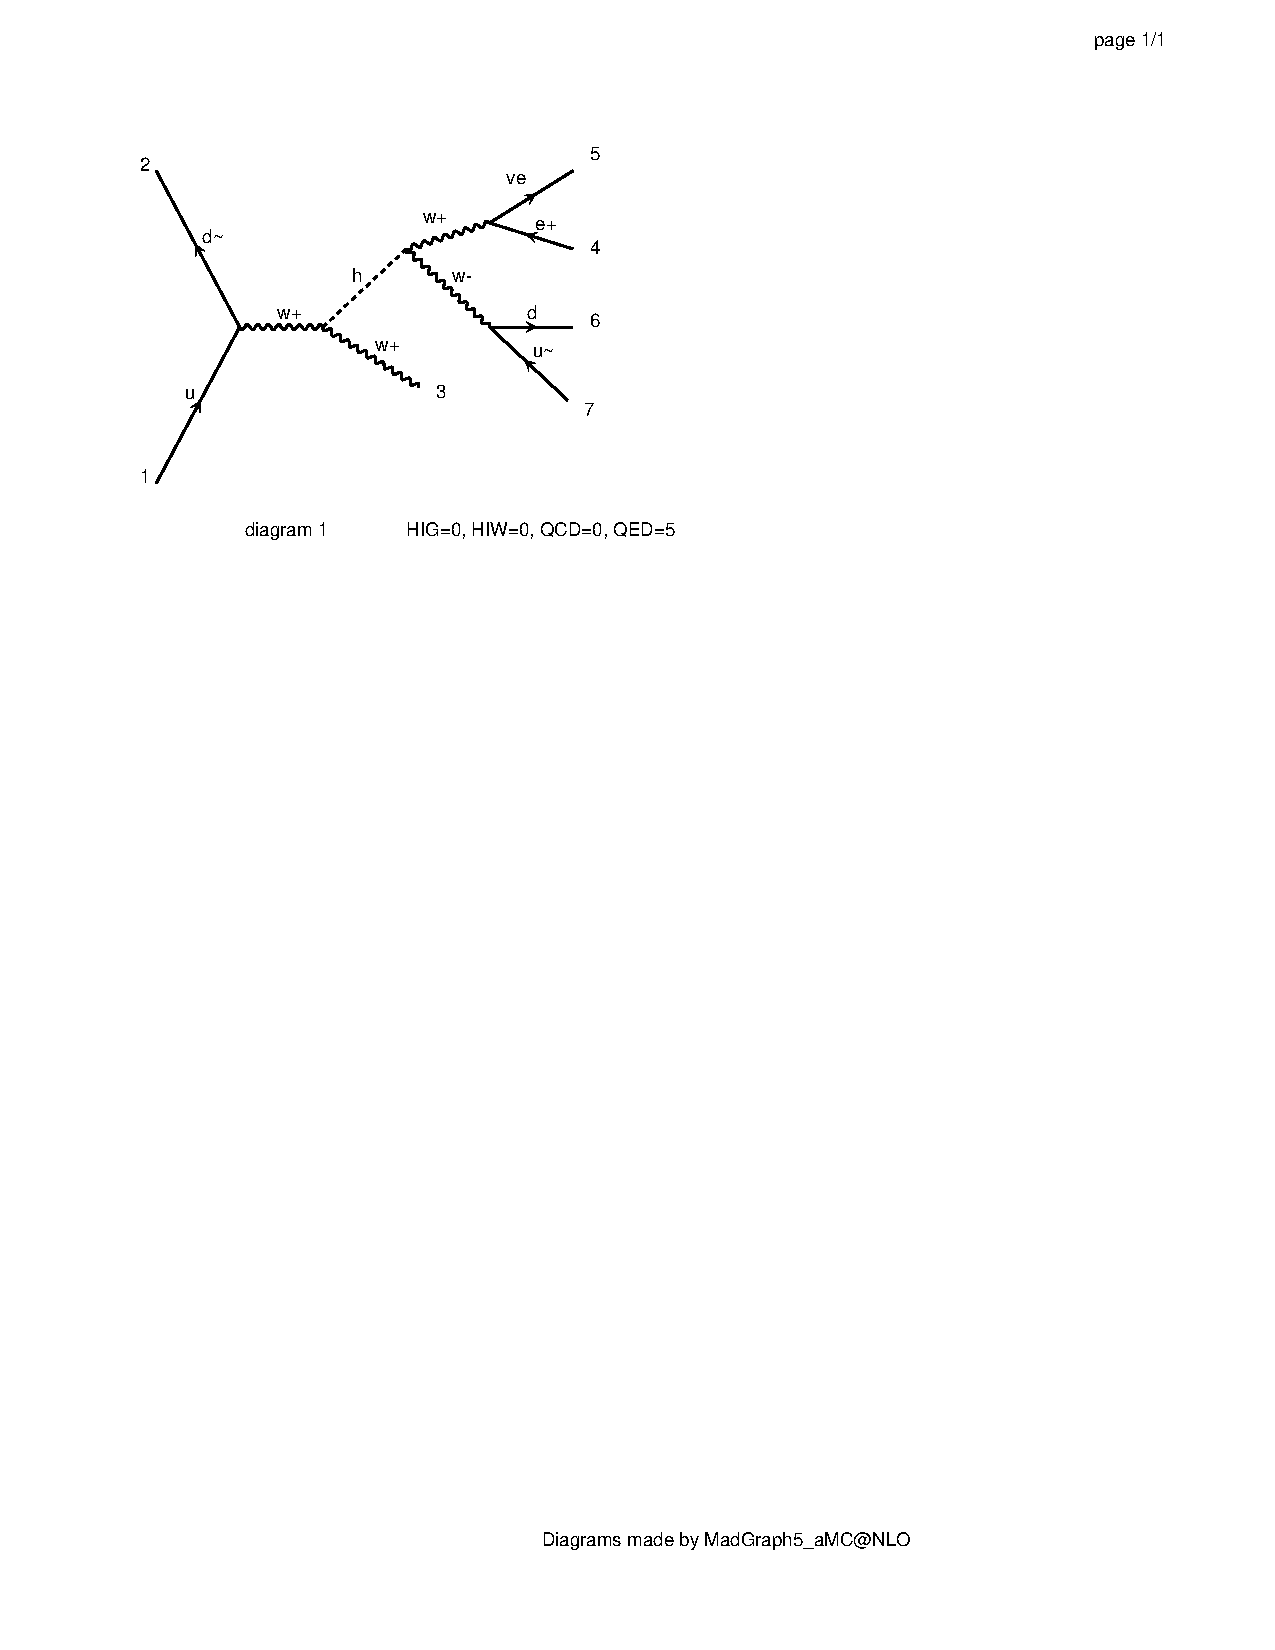
\includegraphics[width=\textwidth,trim={0.5in 7.25in 4in 2cm},clip]{\figpath/Chapter5/MadGraph/matrix_WH.pdf}
    \end{subfigure}
    \caption{Feynman diagrams used to calculate the matrix element probabilities for the \ggH and \WH signals for two-jet events.}
    \label{fig:MadGraph5_example_signal}
\end{figure}

\begin{figure}[!hbt]
    \centering
    \begin{subfigure}[t]{0.9\textwidth}
        \includegraphics[width=\textwidth,page=1,trim={0 3cm 0 2cm},clip]{\figpath/Chapter5/MadGraph/matrix_Wjj.pdf}
    \end{subfigure}

    \begin{subfigure}[t]{0.9\textwidth}
        \includegraphics[width=\textwidth,page=2,trim={0 7.25in 0 2cm},clip]{\figpath/Chapter5/MadGraph/matrix_Wjj.pdf}
    \end{subfigure}
    \caption{A sampling of Feynman diagrams used to calculate the $\W+\cPj\cPj$ matrix element probabilities for two-jet events.}
    \label{fig:MadGraph5_example_Wjj}
\end{figure}

Diagrams with more than two jets present a problem for the matrix element calculations because they doesn't have the same final state as the signal.
As was stated in section~\ref{sec:higgs_production}, for a \ttbar event to pass as a two jet event it must mean that some of the jets are missed.
This can happen in two different ways; either both \W bosons decay leptonically and one lepton is not detected or one of the \W bosons decays hadronically and two of the four jets are missed.
If we really confine the matrix element to two jets, then we can use the diagram with one leptonically decaying \W boson where the other \W is simply not observed (i.e. it decays outside our acceptance).
In this case there are three additional unknown momentum components coming from the \W boson which must be integrated over.
If a third jet were allowed, then the the typical semileptonic \W boson decay is used and one of the light quarks is assumed to be missed.
This also adds three additional integrations to the calculation.
Although it would have been nice to include a \ttbar matrix element probability for discrimination purposes, the additional integrals proved too costly to compute.
Each \ttbar probability took over two minutes to compute, even using accelerated numerical integration packages.
Therefore we did not compute the \ttbar probability and we rely on the signal probabilities being relatively low for \ttbar events.

\begin{figure}[!hbt]
    \centering
    \includegraphics[width=\textwidth]{\figpath/Chapter5/TTbarMEFeynmanDiagrams.png}
    \caption{Feynman diagrams used to calculate top pair probabilities for two- and three-jet events. The circled particles are assumed to be unobserved and an integral is taken over their momenta. Figure and caption from~\cite{Dong2008}.}
    \label{fig:TTbarMEFeynmanDiagrams}
\end{figure}

\subsection{Combinatorial Considerations}


\begin{comment}
Peter:
Several of the diagrams have ambiguities in their final state: for example, the s-channel has two kinematically distinct bottom quarks in the final state. Choosing which jet should be matched to a given parton is difficult; this analysis solves the problem by calculating the differential cross section under both assumptions and adding the answers together. However, in the case of the t-channel diagram, the tagging information is used to match the final-state bottom quark to the tagged jet, improving the sensitivity of the calculation.

The combinations of matching jets to quarks are chosen based on the principle that heavy quarks should be matched to tagged jets whenever possible. In cases of ambiguity, all different combinations are tried. This is true except in the case of the top pair diagram, which has
too many ambiguities and is too computationally expensive to try all
combinations. In this case, only the two combinations of assigning tagged jets to bottom quarks are calculated.
\end{comment}



\subsection{Numerical Integration}

Obviously the differential cross section must be calculated many times for every in both the data and MC samples.
The integration is performed over the neutrino longitudinal momentum, the jet energies, and in some cases over the momenta of missing particles, as in the case of \ttbar.
The result is an integral with dimensionality of anywhere between three and seven dimensions; six in the case of top pair production with a two-jet final state.
These types of equations can't be solved analytically, so we must instead use numerical integration techniques. 

for simpler integrals (3 dimensions) without missing particles
For the simpler cases involving three integrals and without any missing particles, integration is performed using the adaptive quadrature~\cite{VANDOOREN1976207} method based on the CERNLIB~\cite{CERNLIB} RADMUL~\cite{GENZ1980295} routine, adapted for ROOT~\cite{Brun:1997pa}, then adapted again for the CDF single top analysis~\cite{Dong2008}.
The algorithm iteratively divides the n-dimensional region to be integrated into equal-sized regions.
At each iteration the uncertainty in each region is estimated and the region with the largest uncertainty is divided in half.
The iterations continue until all of the regions have an error less than a user specified amount.
In this analysis we used 1\% for all of the matrix elements except for ZLight, where a 5\% uncertainty is allowed.
After the stopping condition is met, the integral in each region is estimated and returned.
This methodThe benefit of using this method is that it is stable and its answers are reproducible; its calculations are deterministic and do not reply on pseudo random number generators (PRNG).
Table~\ref{tab:ME_computation_time_per_event} lists the computation times for each matrix element averaged over 1000 events computed in both the \Wjets and \ggH samples.

\begin{table}[htbp]
\centering
\begin{tabular}{lrr} \hline
Diagram                                & \Wjets Sample [s] & \ggH \joinsym{\MH}{=}{125\gev} Sample [s] \\\hline
\ggH                                   & 2.9               & 3.2   \\
\WH                                    & 4.5               & 3.8   \\
QCD                                    & 0.4               & 0.5   \\
Single Top \cPqs-channel               & 4.2               & 4.3   \\
Single Top \cPqt-channel               & 2.9               & 3.3   \\
$\W\cPqb\cPqb$                         & 1.9               & 1.3   \\
$\W\cmsSymbolFace{L}\cmsSymbolFace{L}$ & 7.4               & 4.8   \\
$\W\cmsSymbolFace{L}\cPqb$             & 2.9               & 2.3   \\
$\W\cmsSymbolFace{L}\cPg$ (LO and NLO) & 3.5               & 2.7   \\
\WW                                    & 1.5               & 1.1   \\
\WZ                                    & 3.9               & 2.9   \\
$\WZ\cPqb\cPqb$                        & 2.5               & 1.9   \\
ZLight                                 & 39.1              & 26.3  \\\hline
Total                                  & 77.7              & 58.5  \\
Total ($\ggH\times35$, $\WH\times14$)  & 233.7             & 217.9 \\\hline
\end{tabular}
\caption{The computations times for each probability averaged over 1000 events and computed in both the \Wjets and \ggH samples. The $\W\cPg\cPg$ diagram was not included in this test. The integration for each of these probabilities was performed using the ROOT integrator.}
\label{tab:ME_computation_time_per_event}
\end{table}

Although the ROOT integrator is deterministic and stable, good qualities in a numerical integrator, it starts to become prohibitively slow for higher dimensional integrals.
Ref.~\cite{Dong2008} performed a test on the \ttbar computation and the ROOT integrator did not converge for a single integration even after running for an entire day.
Instead, the DIVONNE algorithm from the CUBA integration library~\cite{Hahn:2004fe}, which is based on CERNLIB’s DIVON4~\cite{Friedman:1981:NPP:355934.355939} function, is used.






\begin{comment}
DIVONNE is a Monte-Carlo-based integrator using stratified sampling to subdivide its regions. Stratified sampling minimizes the variance of the Monte Carlo events thrown in a given subregion. The Koksma-Hlawka inequality [90] shows that the variance is bounded by half the volume of the subregion times the difference of the supremum and infimum of the function in that subregion. The borders of the subregion are adjusted to reduce this spread. Once a requested variance is reached, the integral is estimated by adding the total of randomly generated points in each subregion.

The implementation of the algorithm in CUBA also samples the subregions independently with the same number of Monte Carlo events in each region. If this result is not consistent with the integral derived already, the regions are subdivided further and the process is repeated.

The DIVONNE algorithm gave results consistent with RADMUL when tested on an
ensemble of a thousand events. It is also very stable: running it repeatedly on an identical event was never observed to change the result by more than 0.001\%.
\end{comment}






\begin{table}[htbp]
\centering
\begin{tabular}{lrr} \hline
Diagram                                & \Wjets Sample [s] & \ggH \joinsym{\MH}{=}{125\gev} Sample [s] \\\hline
Single Top \cPqt\W-channel             & 100.9             & 68.0  \\
\ttbar                                 & 134.7             & 133.6 \\\hline
Total                                  & 235.6             & 201.6 \\\hline
\end{tabular}
\caption{The computation times for the unused single top and \ttbar diagrams. Including these would have doubled the overall computation time. The integration for each of these probabilities was performed using the DIVONNE integrator.}
\label{tab:ME_computation_time_per_event_not_used}
\end{table}

Even with the DIVONNE algorithm, the computation times for the \ttbar and single top $\cPqt\W$ channel ME probabilities were prohibitively large (see table~\ref{tab:ME_computation_time_per_event_not_used}) and were thus dropped from the list of computations.
Besides the \joinsym{\MH}{=}{125\gev} \ggH and \WH diagrams, 34 additional \ggH and 13 additional \WH probabilities were calculated corresponding to different Higgs mass hypotheses.
In the end, however, these probabilities were not used.
The total computation time for a single event was around four minutes, give or take some time for computing cluster overhead.
This computation is by far the most time consuming aspect of this analysis, especially with tens of millions of events to process.
The total computation time ended up costing $\sim$12 million CPU hours and spanned over 1.5 years, requiring the work of several analyzers and the entire Worldwide LHC Computing Grid (WLCG).

\subsection{Standalone Matrix Element Based BDT}

%The Matrix Element Method (MEM) takes into account all final state particle kinematics and correlations to give an estimate, probability density $P_{i}$ , that an event with a given final state comes from process $i$.
The fifteen probabilities $P(x;\alpha)$, corresponding to the leading order diagrams of the major background and signal processes, were computed for each event in both data and MC.
Now that all of the leading order kinematics are encoded in these 15 numbers, they must be combined in order to discriminate signal from background.
A BDT was used rather than combining the ME into a likelihood as in the Matrix Element Likelihood Analysis (MELA) used by $\HZZ\rightarrow\text{4}\Pl$ or the event probability discriminants (EPD) used by the single top analysis done by CDF~\cite{Dong2008}.
Three new BDTs were trained using the same settings as the BDTs with kinematic variables used as inputs.
However, this time the inputs consisted of the 15 matrix element probabilities.
The output discriminant distributions can be found in appendix~\ref{appendix:BDT_Outputs}.
Unfortunately, these BDTs (MEBDT), on their own, did not out perform the kinematic variable based BDTs (KinBDT).
This might be due to the fact that we only used leading order diagrams (not even all of the diagrams), it might have to due with the combinatorics of the jets and partons, or it could have to do with sub-optimal transfer functions.
However, by comparing the KinBDT to the MEBDT, we found that they had complimentary information.

\subsection{Combined BDT}

In order to combine the complimentary information from the kinematic variables and the MEs, with the purpose of discriminating a Higgs event from a background event, we combined the two sets of variables.
An initial BDT was computed which combined the information from 15 of the computed MEs, as noted above.
This gives a less discriminating shallow network the ability to create a better performing network because the inputs are already non-linear variables.
The output of this BDT, along with previously selected kinematic variables, is then used as the input to a new BDT in order to combine all of this complimentary information.
The combined BDT (KinMEBDT) has more discrimination power than either the MEs or the kinematic variables alone.
Images of the output discriminant can be found in appendix~\ref{appendix:BDT_Outputs}.















































\section{Systematic Uncertainties}

The input to the statistical analysis is a set of BDT discriminant histograms and their associated systematic uncertainties.
Given that this is a shape analysis, it is important to consider systematic uncertainties that may change the expected yields (rate changes), the shape of the discriminating variable, or both.
We consider many sources of uncertainty on both the background estimation and the signal normalization.
Table~\ref{tab:systematics_summary} summarizes all of the systematic uncertainties considered for this analysis, with one systematic per line.
The largest uncertainty comes from the \Wjets normalization stemming from the QCD and \Wjets rate estimation.
Each source of systematic uncertainty will be described in more detail in the sections below.

\begin{sidewaystable}[htbp]
\centering
\begin{tabular}{lccl}%
\hline
Source                                            & Type  & Rate Uncertainty [\%] & Notes \\
\hline
QCD Scale (\ggH)                                  & lnN   & 7-8         & Scale uncertainty for NLO \ggH prediction \\
QCD Scale (\qqH)                                  & lnN   & 0.2         & Scale uncertainty for NLO \qqH prediction \\
QCD Scale (\ZH)                                   & lnN   & 1           & Scale uncertainty for NLO \ZH prediction \\
QCD Scale (\WH)                                   & lnN   & 3.1         & Scale uncertainty for NLO \WH prediction \\
QCD Scale (\ttH)                                  & lnN   & 4-9         & Scale uncertainty for NLO \ttH prediction \\
\hline
PDF ($\cPg\cPg$)                                  & lnN   & 6-7         & PDF uncertainty for $\cPg\cPg$ initiated processes (\ggH, \ttH) \\
PDF (\qqbar)                                      & lnN   & 2.6-2.8     & PDF uncertainty for \qqbar initiated processes (\qqH, \WH, \ZH) \\
\hline
QCD Scale (\ttbar)                                & lnN   & 5.7         & Scale uncertainty for NLO \ttbar prediction \\
QCD Scale (\Zjets)                                & lnN   & 3.4         & Scale uncertainty for NLO \Zjets prediction \\
QCD Scale (Single \cPqt)                          & lnN   & 5           & Scale uncertainty for NLO single top prediction \\
QCD Scale (\VV)                                   & lnN   & 3           & Scale uncertainty for NLO diboson prediction \\
\hline
\Wjets Normalization                              & lnN   & 0.4-0.5     & Scale uncertainty for \Wjets prediction \\
QCD                                               & lnN   & 10          & Scale uncertainty for data-driven QCD prediction \\
\ttbar                                            & lnN   & 3           & Scale uncertainty for \ttbar prediction \\
\hline
Luminosity $8\unit{TeV}$                          & lnN   & 2.6         & Signal and all backgrounds \\
Lepton Efficiency                                 & lnN   & 2           & Signal and all backgrounds \\
\ETslash                                          & lnN   & 0.2         & Signal and all backgrounds \\
Jet Energy Scale                                  & shape & 0-20        & Signal and all backgrounds \\
Pileup Weight                                     & shape & 0-8         & Signal and all backgrounds \\
CSV Weight                                        & shape & 0-17        & Signal and all backgrounds \\
Top \pt Weight                                    & shape & 0.5-2       & \ttbar only \\
ME Matching                                       & shape & -           & \Wjets only \\
$\text{Q}^{2}$ Scale                              & shape & -           & \Wjets only \\
\costhetal Weight                                 & shape & -           & \Wjets only \\
QCD Multijet $\eta$ Weight                        & shape & 6-30, 0.5-1 & QCD and \Wjets only \\
\hline
\end{tabular}
\caption{Summary of the systematic uncertainties used in this analysis.}
\label{tab:systematics_summary}
\end{sidewaystable}

\subsection{LHC Luminosity}

A flat rate uncertainty of 2.6\% is applied to all of the simulated samples to account for the uncertainty on the LHC luminosity and thus the simulation normalizations~\cite{CMS-PAS-LUM-13-001}.

\subsection{Sample Cross Sections}

The uncertainties on the theoretical cross sections used for the normalizations of the background simulations are taken from~\cite{SMCrossSectionsat8TeV}.
Likewise, the signal cross sections, branching ratios, and uncertainties are taken from CERN Yellow Report 3~\cite{HiggsCrossSectionsAt8TeVRepot3}.
The uncertainties on the background sample cross sections ranged from 3-5.7\% while the signal cross section uncertainties range from 10-11\% (PDF \& QCDScale).
The theoretical cross section uncertainties on the signal are broken into two components, the uncertainty on the QCD renormalization and factorization scales and the uncertainty on the PDFs.
Table~\ref{tab:cross_section_uncertainties} shows a summary of the uncertainties used.
An additional uncertainty of $\sim$0.5\% is assigned to the \Wjets backgrounds due to the uncertainty from the fit when determining the QCD sample normalization.

\begin{sidewaystable}[htbp]
\centering
\begin{tabular}{lccccccccccc}
\hline
\multirow{2}{*}{Process} & \multicolumn{2}{|c|}{PDF} & \multicolumn{5}{c|}{QCD Scale} & \multicolumn{4}{c}{QCD Scale} \\
\cline{2-12}
& \multicolumn{1}{|c}{\cPg\cPg} & \multicolumn{1}{c|}{\qqbar} & \ggH & \qqH & \WH & \ZH & \multicolumn{1}{c|}{\ttH} & \ttbar & \V & \VV & Single \cPqt \\
\hline
Single \cPqt   &         &           &       &       &     &       &         &       &       &     & 5\% \\
\Zjets         &         &           &       &       &     &       &         &       & 3.4\% &     &     \\
Diboson        &         &           &       &       &     &       &         &       &       & 3\% &     \\
\ttbar         &         &           &       &       &     &       &         & 5.7\% &       &     &     \\
\ggH           & 7-7.5\% &           & 7-8\% &       &     &       &         &       &       &     &     \\
\qqH           &         & 2.6-2.8\% &       & 0.2\% &     &       &         &       &       &     &     \\
\WH, \ZH, \ttH &         &           &       &       & 1\% & 3.1\% & 3.8-9\% &       &       &     &     \\
\hline
\end{tabular}
\caption{Uncertainties on the theoretical cross sections of the simulated signals and backgrounds.}
\label{tab:cross_section_uncertainties}
\end{sidewaystable}

\subsection{MET Uncertainty}

With respect to \ETslash, this analysis follow along the same line as the high mass \lvjj group.
Although we lowered the cut to be \joinsym{\ETslash}{\geqslant}{25\gev}, the uncertainty on the \ETslash should be similar.
Thus we applied the same conservative estimate of a 0.2\% uncertainty.

\subsection{Lepton Selection and Trigger Efficiency}

This analysis makes use of the single lepton triggers and requires a tight electron or muon in the event.
Consequently we must account for any mis-modeling of the lepton identification or trigger efficiencies.
A flat 1\% uncertainty on the trigger efficiency is applied per~\cite{CMS-PAS-HIG-13-027}.
A flat 2\% uncertainty is applied for the lepton selection.

\subsection{Pileup Weights}
The necessity of the pileup weights were discussed in section~\ref{sec:pileup_reweighting}.
The number of pileup interactions in a single bunch crossing is given by:
\begin{equation}
  N_{i}=\frac{\mathcal{L}\cdot\sigma_{\text{minimum bias}}}{v_{\text{orbit}}},
\end{equation}
where $\mathcal{L}$ is the instantaneous luminosity, $\sigma_{\text{minimum bias}}$ is the total minimum bias cross section for an event at the LHC, and $v_{orbit}$ is the LHC orbit frequency (11246\unit{Hz}).
In this calculation and the calculation of the pileup weights the minimum bias cross sections is used, but it's true value is not known.

In order to asses the effect of a systematic uncertainty due to choice of $\sigma_{\text{minimum bias}}=69.3\unit{mb}$, a $\pm$7\% variation was used and the pileup weights were recalculated.
Once that was done, the BDT templates were created again.
As it turns out, the shape changes were negligible, but the rate changes due to this shift can be seen in table~\ref{tab:PUWeight_Uncertainties}.

\begin{table}[htbp]
\centering
\begin{tabular}{lccc} \hline
Process                                    & 2 Jets    & 3 Jets  & $\geqslant$4Jets \\\hline
Diboson                                    & 2-5\%     & 3-6\%   & 3.5-7\%   \\
\Wjets                                     & 3\%       & 4\%     & 4\%       \\
\Zjets                                     & 7-8\%     & 7-8\%   & 7-8\%     \\
\ttbar                                     & 2\%       & 2\%     & 2\%       \\
Single \cPqt                               & 1-3\%     & 2-8\%   & 2-9\%     \\
Multijet                                   & 0-2\%     & 0-3\%   & 0-4\%     \\\hline
\ggH; $\MH=\text{125}\gev$, \HWW           & 2-3\%     & 3\%     & 3.5\%     \\
\qqH; $\MH=\text{125}\gev$, \HWW           & 0.5-3\%   & 1-3.5\% & 2.5-4\%   \\
\WH, \ZH, \ttH; $\MH=\text{125}\gev$, \HWW & 0-3\%     & 1-3\%   & 2-3.5\%   \\\hline
\WH, \ZH, \ttH; $\MH=\text{125}\gev$, \HZZ & 0.5-3\%   & 2-4\%   & 2-4\%     \\
\WH; $\MH=\text{125}\gev$, \Hbb, \Wlv      & 0.5-3\%   & 2-4\%   & 3.5-4.5\% \\
\ttH; $\MH=\text{125}\gev$, \Hbb           & 1.5-4.5\% & 0-2.5\% & 2-4\%     \\\hline
\end{tabular}
\caption{Change in the expected yields due to the pileup weight uncertainties.}
\label{tab:PUWeight_Uncertainties}
\end{table}

\subsection{Jet Energy Scale (JES)}

The jet energy corrections used to correct the jet energy scale back to the particle level were discussed in section~\ref{sec:jets}.
The uncertainty on this correction originates from several uncorrelated sources, but for simplicity we use the total combined uncertainty.
For $M$ uncorrelated sourced the total uncertainty $S\left(\pt,\eta\right)$ is given by:
\begin{equation}
  S\left(\pt,\eta\right)=\sqrt{\sum_{i}^{M}s_{i}^{2}\left(\pt,\eta\right)},
\end{equation}
where $s_{i}\left(\pt,\eta\right)$ is the uncertainty for a single source $i$.
To evaluate the effect this uncertainty has on the BDT discriminant we create the same distribution, but with the jet energies shifted by $\pm1\sigma$ using the procedures given in~\cite{JECUncertainties,JECUncertaintySources}.
This is done before placing a cut on the \pt of the jets so as to allow for migration of events between jet bins.
Some jets that once failed the \pt cut may not pass and some jets might then fail the \pt cut.
Fig.~\ref{fig:JESShift_KinMEBDT} shows the the type of variations expected for the signal (\ggH) and background (\Wjets) samples.
Additionally, table~\ref{tab:JES_Uncertainties} lists the size of the JES uncertainty within each jet bin.

\begin{figure}[!hbt]
    \centering
    \begin{subfigure}[t]{0.48\textwidth}
        \includegraphics[width=\textwidth]{\figpath/Chapter5/Systematics/JESShift_KinMEBDT_ggH125.eps}
        \caption{}
        \label{fig:JESShift_KinMEBDT_ggH125}
    \end{subfigure}
    \begin{subfigure}[t]{0.48\textwidth}
        \includegraphics[width=\textwidth]{\figpath/Chapter5/Systematics/JESShift_KinMEBDT_WJets.eps}
        \caption{}
        \label{fig:JESShift_KinMEBDT_WJets}
    \end{subfigure}
    \caption{Combined kinematic and ME BDT discriminant distributions in the 2 jet, electron bin for the (a) \ggH and (b) \Wjets samples. The black line shows the nominal yield while the red and blue lines show the change in shape if the JES is scales up and down by $1\sigma$, respectively. The yields for the shifted samples are normalized to that of the nominal yield.}
    \label{fig:JESShift_KinMEBDT}
\end{figure}

\begin{table}[htbp]
\centering
\begin{tabular}{lccc} \hline
Process                                    & 2 Jets  & 3 Jets  & $\geqslant$4Jets \\\hline
Diboson                                    & 1-2\%   & 2\%     & 2\%     \\
\Zjets                                     & 0-5.5\% & <1\%    & <1\%    \\
\ttbar                                     & 8-19\%  & 4-7\%   & 2-4\%   \\
Single \cPqt                               & 2-0\%   & <1\%    & <1\%    \\\hline
\ggH; $\MH=\text{125}\gev$, \HWW           & 0-5\%   & 0-2\%   & 0-3\%   \\
\qqH; $\MH=\text{125}\gev$, \HWW           & <1\%    & 4\%     & 7\%     \\
\WH, \ZH, \ttH; $\MH=\text{125}\gev$, \HWW & 2-3\%   & 0-5\%   & 5-8\%   \\\hline
\WH, \ZH, \ttH; $\MH=\text{125}\gev$, \HZZ & 1.5\%   & 0-6\%   & 4-5\%   \\
\WH; $\MH=\text{125}\gev$, \Hbb, \Wlv      & 8-9\%   & 1-10\%  & 2-13\%  \\
\ttH; $\MH=\text{125}\gev$, \Hbb           & 4-17\%  & 11-24\% & 18-21\% \\\hline
\end{tabular}
\caption{Change in the expected yields due to the JES uncertainties.}
\label{tab:JES_Uncertainties}
\end{table}

\subsection{CSV Weights}

Recommendation for how to treat the systematic uncertainties on the CSV weights were given by~\cite{CMS-AN-13-130}, which also details their derivation.
In this analysis, however, the CSV weights were found to be very small and any change in them would have a negligible impact.
It was decided to use a much simpler, yet conservative approach by.
We overestimated the error by using $\text{weight}^{2}$ as the $+1\sigma$ variation and the unweighted distributions as the $-1\sigma$ variation.
The changes to the rate due to this methodology can be seen in table~\ref{tab:CSV_Uncertainties}.

\begin{table}[htbp]
\centering
\begin{tabular}{lccc} \hline
Process                                    & 2 Jets  & 3 Jets    & $\geqslant$4Jets \\\hline
Diboson                                    & 0.5-2\% & 1-3.5\%   & 1-5\%   \\
\Wjets                                     & 0-3\%   & 0-5.5\%   & 0-8.5\% \\
\Zjets                                     & 2-5\%   & 0-5.5\%   & 2-5\%   \\
\ttbar                                     & 5-11\%  & 6-14\%    & 6-17\%  \\
Single \cPqt                               & 4-9\%   & 4-12\%    & 5-16\%  \\\hline
\ggH; $\MH=\text{125}\gev$, \HWW           & 1-3\%   & 1-5\%     & 1-7\%   \\
\qqH; $\MH=\text{125}\gev$, \HWW           & 0-2\%   & 1.5-2.5\% & 2-4\%   \\
\WH, \ZH, \ttH; $\MH=\text{125}\gev$, \HWW & <1\%    & <1\%      & <1\%    \\\hline
\WH, \ZH, \ttH; $\MH=\text{125}\gev$, \HZZ & <1\%    & <1\%      & <1\%    \\
\WH; $\MH=\text{125}\gev$, \Hbb, \Wlv      & <1\%    & <1\%      & <1\%    \\
\ttH; $\MH=\text{125}\gev$, \Hbb           & <1\%    & <1\%      & <1\%    \\\hline
\end{tabular}
\caption{Change in the expected yields due to the CSV weight uncertainties.}
\label{tab:CSV_Uncertainties}
\end{table}

\subsection{Top \texorpdfstring{\pt}{pT}}

As discussed in section~\ref{sec:topPt_reweighting}, the top-quark-pair cross section analyses found that the \pt spectrum of top quarks in data is softer than those in simulation.
Thus we needed to reweight the top quark \pt spectrum in the \ttbar sample.
In order to fully cover any uncertainty on the weights a 100\% uncertainty is assumed.
This means the one standard deviation up and down variations on the weights are taken to be:
\begin{align}
  +1\sigma: {}& ~w_{\text{up}}=w_{\text{TopPt}}{\cdot}w_{\text{TopPt}}, \\
  -1\sigma: {}& ~w_{\text{down}}=1.
\end{align}
This was the recommendation as provided by the TOP PAG~\cite{TopPtReweighting} and results in an uncertainty of 0.5-2.1\% on the \ttbar yield.

\subsection{\texorpdfstring{\costhetal}{CosThetaL} Weight Uncertainty}

Once again we assumed a 100\% uncertainty on the \costhetal weights.
The one standard deviation up and down variations on the weights are taken to be:
\begin{align}
  +1\sigma: {}& ~w_{\text{up}}=w_{\costhetal}{\cdot}w_{\costhetal}, \\
  -1\sigma: {}& ~w_{\text{down}}=1.
\end{align}
These weights are then used as an uncertainty for the \Wjets sample.
As this is not a cut on the events and no change in selection has been made, this does not correspond to a change in the rate, only the \Wjets shape.

\begin{figure}[!hbt]
    \centering
    \begin{subfigure}[t]{0.31\textwidth}
        \includegraphics[width=\textwidth]{\figpath/Chapter5/Systematics/Shape_KinMEBDT_jets2_electron_CMS_hww_lnujj_CosThetaLWeight_shape_WJets.eps}
        \caption{}
        \label{fig:costhetal_uncertainty_jets2}
    \end{subfigure}
    \begin{subfigure}[t]{0.31\textwidth}
        \includegraphics[width=\textwidth]{\figpath/Chapter5/Systematics/Shape_KinMEBDT_jets3_electron_CMS_hww_lnujj_CosThetaLWeight_shape_WJets.eps}
        \caption{}
        \label{fig:costhetal_uncertainty_jets3}
    \end{subfigure}
    \begin{subfigure}[t]{0.31\textwidth}
        \includegraphics[width=\textwidth]{\figpath/Chapter5/Systematics/Shape_KinMEBDT_jets3_electron_CMS_hww_lnujj_CosThetaLWeight_shape_WJets.eps}
        \caption{}
        \label{fig:costhetal_uncertainty_jets4}
    \end{subfigure}
    \caption{Changes to the shape of the BDT discriminant for the \Wjets sample due to variations on the \costhetal weights for the (a) 2 jets bin, (b) 3 jet bin, and (c) $\geqslant$4 jet bin.}
    \label{fig:costhetal_uncertainty}
\end{figure}

\subsection{\Wjets Shape Uncertainties}

In order to take into account variations on the $\text{Q}^{2}$ scale and matrix element parton matching new samples are generated, since these uncertainties cannot be applied after the generation stage.
The samples used are listed in table~\ref{tab:WJets_Shape_Systematic_Samples}.
Since \Wjets is our dominant background in all jet and lepton bins, it was deemed sufficient to apply the $\text{Q}^{2}$ and matching uncertainties only for this sample; generating new samples and/or processing existing large samples for all of the signals and backgrounds would be time consuming and would result in little to no change in the results.

The centrally produced \Wjets events were generated using \textsc{Mad}\textsc{Graph}, a matrix element level generator, which was then interfaced to \textsc{pythia} to model the parton shower with its soft and collinear radiation.
Because \textsc{Mad}\textsc{Graph} generates tree-level diagrams a variation of the factorization and renormalization scales has a significant impact on the simulation.
In this case the scales were varied by a factor of two.

Once the four samples listed in the table were processed, they went through the same selection and weighting procedure as the nominal \Wjets sample.
The new template histograms include only shape changes as the rate uncertainty for the nominal \Wjets same is included in a different source.

\begin{table}[htbp]
\centering
\begin{tabular}{llr} \hline
Sample & Dataset Name & Cross Section \\\hline
ME Matching Up                  & /WJetsToLNu\_matchingup\_8TeV-madgraph-tauola & 37509\unit{pb} \\
ME Matching Down                & /WJetsToLNu\_matchingdown\_8TeV-madgraph-tauola & 37509\unit{pb} \\
Q\textsuperscript{2} Scale Up   & /WJetsToLNu\_scaleup\_8TeV-madgraph-tauola & 37509\unit{pb} \\
Q\textsuperscript{2} Scale Down & /WJetsToLNu\_scaledown\_8TeV-madgraph-tauola & 37509\unit{pb} \\\hline
\end{tabular}
\caption{Samples used for \Wjets systematic shape uncertainties. Each dataset name is appended with /Summer12\_DR53X-PU\_S10\_START53\_V7A-v1/AODSIM.}
\label{tab:WJets_Shape_Systematic_Samples}
\end{table}

\subsection{QCD \texorpdfstring{$\eta$}{eta} Weights Uncertainty}

The uncertainty on the weights as a function of $\eta$ for the data-driven QCD sample have to do with the choice of selection criteria, which was first discussed in section~\ref{sec:QCD_data-driven_sample}.
The motivation for the chosen isolation windows was more practical than due to some deeper, underlying physics.
Therefore the uncertainties for the weights are generated by varying the isolation criteria and creating alternate QCD samples with a modified set of events.
One side of the isolation region was relaxed at a time to generate four new samples, two each for the electron and muon channels.
These samples were then used to generate four new sets of weights, just as done in section~\ref{sec:QCD_reweighting}.
The resulting samples lead to a small variation in the QCD template shapes, but also lead to an uncertainty on the QCD yield of 6-30\% and on the \Wjets yield of 0.1-0.5\%.
